%% =====================================================================
%%  GPS-Denied Autonomous UAV Navigation - project report source
%%  Compile with pdfLaTeX (Overleaf default). Main file: main.tex
%% =====================================================================
\documentclass[10pt,a4paper]{article}

%% ---------- Packages -------------------------------------------------
\usepackage[utf8]{inputenc}
\usepackage{amsmath,amssymb,bm}
\usepackage{graphicx}
\usepackage{booktabs}
\usepackage{tabularx}
\usepackage{longtable}
\usepackage{multirow}
\usepackage{array}
\usepackage{makecell}
\usepackage[table]{xcolor}
\usepackage{siunitx}
\usepackage{enumitem}
\usepackage{float}
\usepackage{listings}
\usepackage{tikz}
\usetikzlibrary{arrows.meta,positioning,shapes.geometric,shapes.misc,fit,calc,backgrounds}
\usepackage{hxstyle}          % journal-style layout (header band, fonts, captions, links)
\usepackage{subcaption}

\graphicspath{{figures/}}
\setlength{\emergencystretch}{2em}   % fewer overfull lines with long identifiers
\sisetup{detect-all, per-mode=symbol, range-phrase=--, range-units=single}
\DeclareSIUnit\gacc{g}
\newcommand{\INR}[1]{\mbox{INR~#1}}
% \code{...}/\topic{...}: verbatim-safe monospace text that may break after '_' and '/'
\ExplSyntaxOn
\tl_new:N \l__rep_code_tl
\cs_new_protected:Npn \__rep_code:n #1
  {
    \tl_set:Nx \l__rep_code_tl { \tl_to_str:n {#1} }
    \exp_args:NNo \tl_replace_all:Nnn \l__rep_code_tl { \c_underscore_str }
      { \c_underscore_str \allowbreak }
    \tl_replace_all:Nnn \l__rep_code_tl { / } { / \allowbreak }
    \texttt { \tl_use:N \l__rep_code_tl }
  }
\NewDocumentCommand \code  { m } { \__rep_code:n {#1} }
\NewDocumentCommand \topic { m } { \__rep_code:n {#1} }
\ExplSyntaxOff
\newcommand{\todo}[1]{\textcolor{red}{[TODO: #1]}}
\newcolumntype{L}{>{\raggedright\arraybackslash}X}
\newcolumntype{Y}{>{\raggedright\arraybackslash}p}

\definecolor{blk1}{HTML}{257DE0}
\definecolor{blk2}{HTML}{F47230}
\definecolor{blk3}{HTML}{00B894}
\definecolor{blk4}{HTML}{6A4CE2}
\definecolor{softgray}{HTML}{F2F2F2}
\definecolor{codebg}{HTML}{F7F7F7}

\lstset{basicstyle=\ttfamily\footnotesize, backgroundcolor=\color{codebg},
  frame=single, rulecolor=\color{black!25}, breaklines=true, columns=fullflexible,
  keepspaces=true, showstringspaces=false, xleftmargin=2pt, xrightmargin=2pt}

\tikzset{
  blk/.style={draw, rounded corners=2pt, align=center, font=\footnotesize,
              minimum height=8mm, inner sep=3pt, fill=white},
  hw/.style={blk, fill=blk1!10, draw=blk1!80!black},
  sw/.style={blk, fill=blk3!10, draw=blk3!70!black},
  ext/.style={blk, fill=blk2!10, draw=blk2!80!black},
  grp/.style={draw=black!45, dashed, rounded corners=4pt, inner sep=7pt},
  arr/.style={-{Stealth[length=2.2mm]}, thick},
  darr/.style={{Stealth[length=2.2mm]}-{Stealth[length=2.2mm]}, thick},
  lbl/.style={font=\scriptsize, fill=white, inner sep=1pt},
  proc/.style={draw, rectangle, rounded corners=2pt, align=center, font=\footnotesize,
               minimum width=36mm, minimum height=7mm, fill=blk1!8},
  dec/.style={draw, diamond, aspect=2.4, align=center, font=\footnotesize,
              inner sep=1pt, fill=blk2!10},
  term/.style={draw, rounded rectangle, align=center, font=\footnotesize,
               minimum width=26mm, minimum height=7mm, fill=blk3!12},
}

%% =====================================================================
%%  Title block (see hxstyle.sty). Authors/affiliations are placeholders: they are
%%  not recorded in the repository. Fill them in before circulating.
%% =====================================================================
\hxtopline{Design Practicum Project (Group 66) \textperiodcentered{} November 2026}
\hxband{Indian Institute of Technology Mandi}
       {GPS-Denied Autonomous UAV Navigation}
       {GITHUB.COM/DEEPAKSINGLA-BYTE/GPS-DENIED-VTOL}
\hxshortauthors{K. Halder, A. Mittal, Deepak, K. Jain, P. Azad, R. Dey, Vamsi}
\hxshorttitle{GPS-denied UAV navigation}

\title{A low-cost, open-source companion-computer architecture for GPS-denied
multirotor navigation: LiDAR--optical-flow sensing, Wi-Fi offloaded Nav2 planning
and hybrid YOLO--SAM perception}
%% Faculty advisor first, then student authors in alphabetical order of name;
%% superscript letters = affiliations below.
\newcommand{\aff}[1]{\textsuperscript{\color{hxlink}#1}}
\author{Dr.~Kaushik Halder\aff{b,$\dagger$}, Arnav Mittal\aff{d}, Deepak\aff{a}, Krish Jain\aff{b}, Pranit Azad\aff{b},
  Reman Dey\aff{c}, Vamsi\aff{a}}
\affiliations{%
  \textsuperscript{a}School of Mechanical and Materials Engineering, Indian Institute of Technology Mandi, Kamand, Himachal Pradesh 175075, India\\
  \textsuperscript{b}School of Computing and Electrical Engineering, Indian Institute of Technology Mandi, Kamand, Himachal Pradesh 175075, India\\
  \textsuperscript{c}School of Physical Sciences, Indian Institute of Technology Mandi, Kamand, Himachal Pradesh 175075, India\\
  \textsuperscript{d}School of Mathematical and Statistical Sciences, Indian Institute of Technology Mandi, Kamand, Himachal Pradesh 175075, India\\
  \textsuperscript{$\dagger$}Faculty advisor}
%% To mark a corresponding author: add ,$\ast$ to that author's \aff{...} and uncomment:
%% \correspondence{\textsuperscript{$\ast$}\,Corresponding author. E-mail address: ...}

\articleinfo{%
  \textit{Version:}\\
  1.0, 25 November 2026
  \infosep
  \textit{Keywords:}\\
  GPS-denied navigation\\ Unmanned aerial vehicle\\ Companion computer\\ ROS~2 and Nav2\\
  Optical flow\\ 2D LiDAR\\ MAVLink\\ Semantic segmentation\\ Open hardware
  \infosep
  \textit{Source repository:}\\
  \href{https://github.com/DEEPAKSINGLA-byte/gps-denied-vtol}{github.com/DEEPAKSINGLA-byte/\\gps-denied-vtol}}
\abstracttext{%% Abstract text only; layout is set by \hxmaketitle in main.tex
Multirotor UAVs lose their GNSS position indoors, underground, under tree canopy and
when signals are jammed, and without an absolute fix inertial navigation drifts
quadratically. We present a low-cost, open-source hardware and software system that
gives a Pixhawk-class multirotor running ArduPilot an independent position and obstacle
reference. A Raspberry Pi on the vehicle streams autopilot telemetry (including optical
flow and rangefinder), 360\textdegree{} YDLIDAR~G2 scans and camera video over Wi-Fi
to a ground laptop running ROS~2 Humble. There, odometry is reconstructed, Nav2 plans
collision-free velocity commands, and a hybrid perception node refines YOLOv8 masks
with Segment Anything~2.1. Commands return through a gated MAVLink path that acts only
in armed \code{GUIDED} mode, is clamped to \SI{0.5}{\metre\per\second} and stops after
\SI{0.5}{\second} without input. Our link optimisations cut command forwarding from
\SI{54}{\milli\second} to \SI{1.4}{\milli\second} and telemetry-to-odometry delay from
\SI{20}{\milli\second} to \SI{2}{\milli\second} (single host). We validated the system with a
bench log of sensor noise and the zero-velocity detector, a dead-reckoning
experiment (\SI{86.5}{\metre} error after \SI{25}{\second} uncompensated), a GPU
perception benchmark (\SI{5.6}{\milli\second} YOLO-only, \SI{31.6}{\milli\second} with
SAM), 17/17 passing unit tests, and 26 simulated flights (\SI{1.7}{h}) against Gazebo ground truth: speed
limits held, height hold was within 3--\SI{14}{cm} RMS, and three explorations
completed, while four office flights fell after propeller contact. On the real vehicle,
Nav2 flew an autonomous square path around trees outdoors at night, and a
\SI{7}{\minute} GNSS-free hover at \SI{2.5}{\metre} over grass drifted \SI{1.6}{\metre}, bounded but over 30 times the
\SI{5}{\centi\metre} target; trajectory accuracy against ground truth is not yet
measured. We also describe a fully onboard stereo-vision design
(\INR{45{,}679} bill of materials) as the next step.
}

%% =====================================================================
\begin{document}

\hxmaketitle

%% ---------------------------------------------------------------------
\section*{Specifications table}
\addcontentsline{toc}{section}{Specifications table}

\vspace{-1mm}
\begingroup
\centering
\footnotesize
\renewcommand{\arraystretch}{1.1}
\begin{tabularx}{\textwidth}{p{0.22\textwidth} L}
\toprule
Hardware name & GPS-Denied Autonomous UAV Navigation Stack (\code{gps-denied-vtol}) \\
Subject area & Engineering and material science; Robotics; Aerospace (unmanned aerial systems) \\
Hardware type & Field measurements and sensors; Robotics and automation; Electrical engineering and computer science \\
Closest commercial analog & No single equivalent. Partial analogues: ModalAI VOXL~2 (onboard VIO), Holybro PX4 Vision kit, Intel RealSense T265 tracking camera (discontinued) \\
Open-source licence & Software: MIT License. Hardware documentation: CERN-OHL-P v2 \\
Cost of hardware & Design target bill of materials: \INR{45{,}678.66} (\cref{tab:bom-target}). Prototype purchases: \INR{52{,}714} (\cref{tab:bom-spend}), plus lab-stock autopilot, LiDAR, camera and battery. \\
Source file repository & \url{https://github.com/DEEPAKSINGLA-byte/gps-denied-vtol} (an archived release with DOI will be created on acceptance) \\
\bottomrule
\end{tabularx}\par
\endgroup

\begin{table}[H]
\centering
\small
\caption{Key technical parameters of the current prototype, as built and configured. Values are configuration limits or measured quantities, as indicated.}
\label{tab:keyparams}
\renewcommand{\arraystretch}{1.15}
\begin{tabularx}{\textwidth}{p{0.36\textwidth} L}
\toprule
\textbf{Parameter} & \textbf{Value (source)} \\
\midrule
Flight controller / firmware & Holybro Pixhawk~6C, ArduPilot (ArduCopter), MAVLink over USB @ 115\,200 baud \\
Airframe / propulsion & F450 quadrotor, A2212 \SI{1000}{KV} motors, \SI{30}{\ampere} ESCs, 1045 propellers, 3S \SI{2200}{\milli\ampere\hour} LiPo \\
Companion computer & Raspberry Pi~5 (4\,GB), Linux, Python~3 (no ROS on the vehicle) \\
Ground computer & Laptop, Ubuntu 22.04, ROS~2 Humble, NVIDIA RTX~4050 Laptop GPU \\
Exteroceptive sensors & YDLIDAR G2 2D LiDAR (\SIrange{0.12}{16}{\metre} accepted, 1\textdegree{} bins); downward optical flow + rangefinder via autopilot; USB~2.0 UVC camera, 640$\times$480 MJPEG \\
Telemetry to ground & UDP JSON, event-driven, up to \SI{30}{\hertz}, $\le$\SI{1400}{B} per datagram \\
LiDAR to ground & UDP binary, \SI{1094}{B} per revolution; $\approx$\SI{7}{\hertz} at \code{/scan} (documented) \\
Video to ground & TCP, JPEG $q{=}70$, \SI{20}{fps} requested; $\approx$\SI{15}{\hertz} at \code{/camera/image_raw} (documented, camera-limited) \\
Command uplink & UDP JSON $\rightarrow$ \code{SET_POSITION_TARGET_LOCAL_NED} (velocity + yaw rate) \\
Command safety envelope & Armed \emph{and} \code{GUIDED} only; $|v_{xy}| \le \SI{0.5}{\metre\per\second}$; \SI{0.5}{\second} stale-command stop; never auto-arms \\
Planner / controller & Nav2: NavFn global planner (\SI{5}{\hertz}), DWB holonomic controller (\SI{10}{\hertz}) \\
Costmaps & Rolling, \SI{0.05}{\metre} cells; local $8\times8$\,m, global $20\times20$\,m; robot radius \SI{0.25}{\metre}; inflation \SI{0.40}{\metre} \\
Perception & YOLOv8n-seg + SAM~2.1-tiny box-prompted refinement; measured \SI{31.6}{\milli\second}/frame at SAM \SI{768}{px} (\cref{sec:val-seg}) \\
Simulation & PX4 SITL + Gazebo Harmonic; x500 with 2D LiDAR; Baylands park and generated 24$\times$16\,m office world \\
\bottomrule
\end{tabularx}
\end{table}

%% ---------------------------------------------------------------------
\section{Introduction and hardware in context}
\label{sec:intro}

\subsection{The GPS-denied navigation problem}

Small multirotor UAVs estimate their state by fusing a low-cost micro-electro-mechanical
(MEMS) inertial measurement unit (IMU) with GNSS position and velocity
\cite{groves2013principles}. GNSS is routinely unavailable or untrustworthy: signals
are blocked in mines, tunnels and buildings, degraded in urban canyons and beneath
foliage, and can be deliberately jammed or spoofed \cite{humphreys2008spoofing}.
When the absolute fix disappears, the vehicle must dead-reckon on the IMU, and the
error of a strapdown solution grows rapidly \cite{titterton2004strapdown}. For an
uncompensated accelerometer bias $\mathbf{b}_a$, double integration gives a position
error
\begin{equation}
  \delta\mathbf{p}(t) \;\approx\; \tfrac{1}{2}\,\mathbf{b}_a\,t^{2},
  \label{eq:bias-drift}
\end{equation}
while a small attitude error $\delta\theta$ projects gravity into the horizontal
channel, adding $\tfrac12 g\,\delta\theta\,t^2$ \cite{titterton2004strapdown}. A residual bias of
only \SI{1}{\milli\gacc} (\SI{9.8e-3}{\metre\per\second\squared}) produces roughly
\SI{0.5}{\metre} of error after \SI{10}{\second} and \SI{18}{\metre} after one minute. \Cref{sec:val-dr} confirms this growth on data
from the prototype's own autopilot. A GPS-denied navigation system must therefore
provide an \emph{exteroceptive} reference (vision, range, radio or field-map matching)
that bounds this drift, together with a means of detecting and avoiding obstacles in
unknown surroundings.

\subsection{Formal statement}

Following our problem statement, the vehicle state at time $t$ is
\begin{equation}
  \mathbf{x}_t = \left[\,\mathbf{p}_t,\;\mathbf{v}_t,\;\mathbf{q}_t,\;\mathbf{b}_a,\;\mathbf{b}_g\,\right],
\end{equation}
comprising position, velocity, attitude quaternion, and accelerometer and gyroscope
biases. Given control/IMU inputs $\mathbf{u}_t$ and exteroceptive measurements
$\mathbf{z}_{t,k}$ (camera features, LiDAR ranges, flow, rangefinder), the
maximum-a-posteriori trajectory is
\begin{equation}
  \mathbf{x}^{*}_{0:T} = \arg\max_{\mathbf{x}_{0:T}}\;
  p(\mathbf{x}_0)\prod_{t=1}^{T} p(\mathbf{x}_t\mid\mathbf{x}_{t-1},\mathbf{u}_t)
  \prod_{k} p(\mathbf{z}_{t,k}\mid\mathbf{x}_t),
  \label{eq:map}
\end{equation}
which is solved recursively by an extended Kalman filter (EKF) or in batch by
factor-graph optimisation \cite{dellaert2017factor}. In the present prototype the
recursive solution is delegated to the autopilot's EKF3 where it is available, and a
lightweight dead-reckoning front-end on the ground computer supplies the planner when
it is not (\cref{sec:design-odom}).

\subsection{Target performance}

We set the key performance indicators (KPIs) in \cref{tab:kpi}. They are
\emph{targets for the final onboard system}. \Cref{sec:discussion} reports how far the
current prototype has been verified against each.

\begin{table}[H]
\centering\small
\caption{Project KPIs (from \code{docs/PROBLEM_STATEMENT.md}).}
\label{tab:kpi}
\begin{tabularx}{\textwidth}{l l L}
\toprule
\textbf{Metric} & \textbf{Target} & \textbf{Typical fallback without GNSS} \\
\midrule
Trajectory error & $<0.5\%$ of distance flown & $>10\%$ \\
Hover drift & $\le\pm\SI{5}{\centi\metre}$ over \SI{10}{\minute} & $\ge\SI{2}{\metre}$ per minute \\
Update rate & state $\ge\SI{100}{\hertz}$, vision $\ge\SI{30}{\hertz}$ & dropped frames break the filter \\
Compute power & $\le\SI{15}{\watt}$, onboard & needs off-board computing \\
Illumination & \SIrange{0}{10000}{lux} and above & fails below \SI{50}{lux} \\
Endurance & $\ge\SI{30}{\minute}$ (objective 8) & -- \\
\bottomrule
\end{tabularx}
\end{table}

\subsection{Background and related work}

\paragraph{Exteroceptive references} Visual and visual--inertial odometry and SLAM
(e.g.\ VINS-Mono \cite{qin2018vins}, ORB-SLAM3 \cite{campos2021orbslam3}) achieve
sub-percent drift with light, inexpensive cameras, but fail in darkness, smoke and on
textureless surfaces. Downward optical-flow sensors with a rangefinder
\cite{honegger2013px4flow} give metric velocity at negligible compute cost but no map.
2D and 3D LiDAR provide illumination-independent geometry and support occupancy-grid
SLAM \cite{macenski2021slamtoolbox} at a weight and power cost. Radio beacons (UWB),
fiducials, magnetic-anomaly (MAGNAV) and terrain-referenced (TERCOM) navigation need
prior infrastructure or maps. Surveys of the space include \cite{balamurugan2016survey}.

\paragraph{Open robotics middleware} ROS~2 \cite{macenski2022ros2} with the Nav2
navigation stack \cite{macenski2020marathon} offers costmaps, global planners, local
controllers such as the dynamic window approach \cite{fox1997dwa}, and behaviour-tree
mission logic \cite{colledanchise2018bt}. PX4 \cite{meier2015px4} and ArduPilot
\cite{ardupilot} are the dominant open autopilots, communicating over MAVLink
\cite{koubaa2019mavlink}.

\paragraph{Gap} Integrated, documented, reproducible GPS-denied systems for hobby-grade
multirotors are rare. Commercial modules with onboard VIO exist but are closed, costly
or discontinued. Academic systems are typically tied to bespoke airframes and high-end
compute. There is a practical need for an \emph{incremental} path: a system that can be
assembled from parts already found in student laboratories, that exposes every signal
for inspection, and that can migrate towards fully onboard processing.

\subsection{Contribution}

Our main contributions are:
\begin{enumerate}[leftmargin=*,itemsep=1pt]
  \item a structured trade study of 15 GPS-denied navigation modalities with
    multi-criteria scoring for three mission profiles (\cref{sec:design-trade});
  \item a companion-computer architecture that adds 2D LiDAR, optical-flow odometry,
    Nav2 planning and semantic perception to an unmodified ArduPilot vehicle, using
    only USB connections on the airframe (\cref{sec:arch});
  \item a latency-engineered Wi-Fi link with single-datagram encodings, QoS marking,
    clock synchronisation and per-stream health metrics (\cref{sec:design-link});
  \item a layered command-safety design: arming and mode gating, speed clamping,
    stale-command stop, a vibration guard and pilot override (\cref{sec:design-safety});
  \item a hybrid YOLO--SAM segmentation module with explicit mask-quality gates and
    unit tests (\cref{sec:design-perception});
  \item a reproducible PX4/Gazebo simulation environment, including a generated office
    world and frontier exploration (\cref{sec:op-sim});
  \item a clear account of what we have and have not yet verified
    (\cref{sec:validation,sec:discussion}).
\end{enumerate}

\subsection{Prototype versus design target}
\label{sec:proto-vs-target}

We describe two hardware configurations, and it is worth keeping them apart:
\begin{description}[leftmargin=1em,itemsep=2pt]
  \item[Current prototype (implemented).] F450 quadrotor with a Pixhawk~6C running ArduPilot, YDLIDAR G2, USB
    camera and autopilot-attached optical flow/rangefinder. A Raspberry Pi streams the
    sensor data to a GPU laptop, which performs estimation, planning and perception.
    All software in \cref{sec:arch,sec:design,sec:build,sec:operation} refers to this
    configuration.
  \item[Design target (specified, not yet built).] A SC132GS stereo camera,
    Raspberry Pi~5 (8\,GB), Holybro Kakute H7 running PX4 and an ELRS radio link, with
    \emph{all} processing onboard (\cref{tab:bom-target}). Our timeline
    (\cref{tab:timeline}) places this in phases~1--6.
\end{description}
Off-board processing is not part of the final design. We use the ground laptop as a
development step, because it lets us watch every intermediate signal while the
algorithms are still being tuned.

%% ---------------------------------------------------------------------
\section{Hardware description and system architecture}
\label{sec:arch}

\subsection{Overview}

The system is split across two computers joined by an IEEE~802.11 link
(\cref{fig:system}). The \emph{airborne segment} contains the flight controller, which
keeps sole authority over attitude stabilisation and motor mixing, and a Raspberry Pi
companion computer that only moves data. It reads the autopilot over MAVLink, the
LiDAR over a USB--serial bridge and the camera over USB Video Class (UVC), and
forwards velocity commands back to the autopilot. The \emph{ground segment} is a
laptop with an NVIDIA GPU running ROS~2 Humble. It performs state reconstruction,
mapping, planning, perception, visualisation and health monitoring.

This division follows from three engineering constraints. (i) The inner control loop
must not depend on the radio link: if Wi-Fi fails the autopilot continues to stabilise
and its own failsafes apply. (ii) The perception workload, roughly \SI{30}{\milli\second}
per frame on a laptop GPU (\cref{sec:val-seg}), is far beyond a Raspberry Pi CPU at
useful frame rates. (iii) During development every intermediate signal should be
observable in RViz and PlotJuggler without loading the vehicle.

\begin{figure}[t]
\centering
\begin{tikzpicture}[x=1cm, y=1cm]
  % ---------------- airborne segment
  \node[ext, minimum width=20mm] (rc)  at (0.2, 1.0) {RC receiver\\(pilot)};
  \node[ext, minimum width=20mm] (esc) at (0.2,-1.0) {ESCs\\+ motors};
  \node[hw, minimum width=33mm] (imu)  at (3.7, 1.35) {IMU, baro, compass (FMU)};
  \node[hw, minimum width=36mm] (fc)   at (3.7, 0.0) {Flight controller\\Pixhawk 6C, ArduPilot EKF3};
  \node[hw, minimum width=33mm] (flow) at (3.7,-1.35) {Optical flow + rangefinder};
  \node[hw, minimum width=28mm, minimum height=24mm] (pi) at (8.4, 0.0)
       {\textbf{Raspberry Pi}\\companion\\[2pt]\scriptsize\code{start_streams.py}};
  \node[hw, minimum width=26mm] (lidar) at (12.2, 0.75) {YDLIDAR G2\\2D LiDAR};
  \node[hw, minimum width=26mm] (cam)   at (12.2,-0.75) {USB camera\\UVC, MJPEG};
  \draw[arr] (imu) -- (fc);
  \draw[arr] (flow) -- (fc);
  \draw[arr] (rc) -- (fc.west |- rc);
  \draw[arr] (fc.west |- esc) -- (esc);
  \draw[darr] (fc) -- node[lbl,above]{USB} node[lbl,below,yshift=-1pt]{MAVLink} (pi);
  \draw[arr] (lidar) -- node[lbl,above]{USB} (pi.east |- lidar);
  \draw[arr] (cam) -- node[lbl,below]{USB} (pi.east |- cam);
  \begin{scope}[on background layer]
    \node[grp, fit=(rc)(esc)(imu)(flow)(pi)(lidar)(cam)] (air) {};
  \end{scope}
  \node[font=\footnotesize\bfseries, anchor=south west] at (air.north west) {Airborne segment};

  % ---------------- radio link
  \node[draw=blk1!70!black, fill=blk1!6, minimum width=15.0cm, minimum height=5mm,
        font=\footnotesize\itshape] (wifi) at (6.45,-3.0) {Wi-Fi 802.11 link (direct, e.g.\ laptop 5\,GHz hotspot)};
  \draw[darr] (pi.south) -- (pi.south |- wifi.north);

  % ---------------- ground segment
  \def\ry{-4.55}
  \node[sw, font=\scriptsize, minimum width=30mm] (cb) at (0.75,\ry)  {\code{mavlink_cmd_bridge}};
  \node[sw, font=\scriptsize, minimum width=30mm] (lr) at (4.55,\ry)  {\code{lidar_udp_receiver}};
  \node[sw, font=\scriptsize, minimum width=30mm] (br) at (8.35,\ry)  {\code{mavlink_to_ros2_bridge}};
  \node[sw, font=\scriptsize, minimum width=30mm] (cr) at (12.15,\ry) {\code{camera_tcp_receiver}};
  \draw[arr, blk2!90!black] (cb.north) -- node[lbl,right]{UDP 14553} (cb.north |- wifi.south);
  \draw[arr, blk1] (lr.north |- wifi.south) -- node[lbl,right]{UDP 14552} (lr.north);
  \draw[arr, blk1] (br.north |- wifi.south) -- node[lbl,right]{UDP 14551} (br.north);
  \draw[arr, blk1] (cr.north |- wifi.south) -- node[lbl,right]{TCP 5000} (cr.north);

  \node[sw, minimum width=40mm, minimum height=11mm] (nav) at (6.45,-6.35)
       {\textbf{Nav2}: rolling costmaps,\\NavFn planner, DWB controller};
  \node[sw, minimum width=28mm, minimum height=11mm] (seg) at (12.15,-6.35)
       {YOLOv8 + SAM~2.1\\(GPU)};
  \draw[arr] (lr.south) -- node[lbl,left]{\topic{/scan}} (lr.south |- nav.north);
  \draw[arr] (br.south) -- node[lbl,right]{\topic{/odom}, TF} (br.south |- nav.north);
  \draw[arr] (cr) -- node[lbl,right]{\topic{/camera/image_raw}} (seg);
  \draw[arr, blk2!90!black] (nav.west) -| node[lbl,pos=0.3,below]{\topic{/cmd_vel}} (cb.south);
  \node[sw, minimum width=150mm, fill=softgray, draw=black!40] (mon) at (6.45,-7.75)
       {\code{metrics_monitor} (\topic{/metrics/*}, \topic{/diagnostics}) \quad
        \code{scan_to_3d} (\topic{/map_3d}) \quad RViz};
  \begin{scope}[on background layer]
    \node[grp, fit=(cb)(lr)(br)(cr)(nav)(seg)(mon)] (gnd) {};
  \end{scope}
  \node[font=\footnotesize\bfseries, anchor=north west] at (gnd.south west)
       {Ground segment: laptop, Ubuntu 22.04, ROS~2 Humble};
\end{tikzpicture}
\caption{System architecture of the implemented prototype. Blue: hardware; green:
ground software nodes; orange: actuators and pilot input. Blue links carry sensor data
down, the orange link carries velocity commands up. The autopilot retains the inner
attitude loop and failsafes, so loss of the Wi-Fi link never removes stabilisation.}
\label{fig:system}
\end{figure}

\subsection{Airborne hardware}

\Cref{fig:hwphoto} shows the assembled prototype with each component labelled.

\begin{figure}[t]
\centering
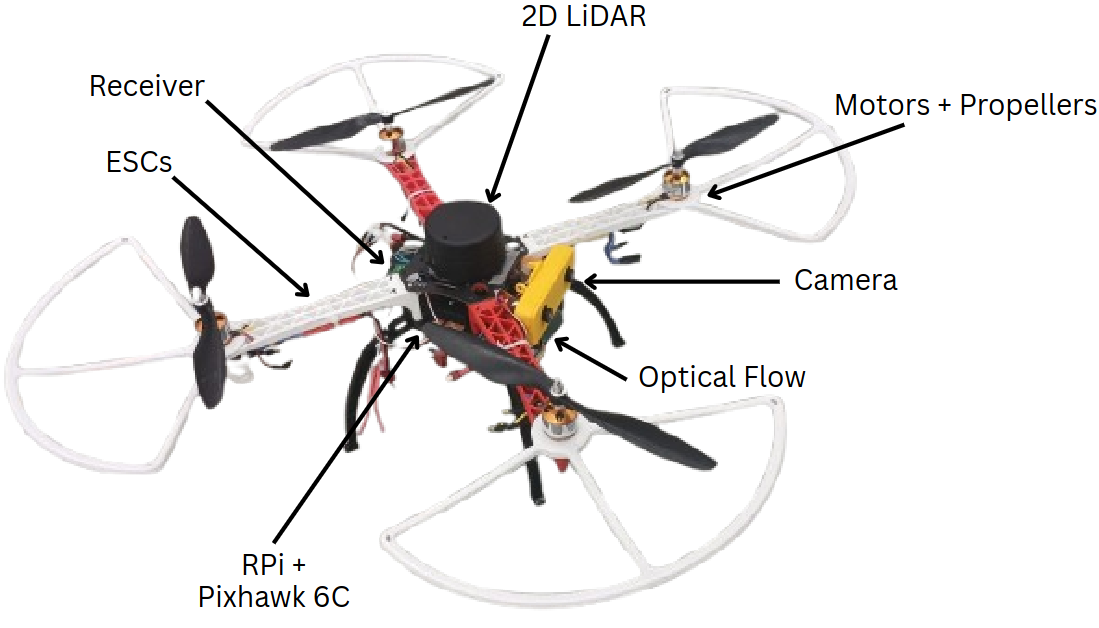
\includegraphics[width=0.9\textwidth]{hardware_pic.png}
\caption{The assembled prototype quadcopter. A 2D LiDAR sits on top of the frame. The
camera and the downward optical-flow sensor are on the front arm. The Raspberry Pi
companion computer and the Pixhawk~6C flight controller are in the centre stack, with
the RC receiver and the ESCs on the frame. Propeller guards are fitted for indoor and
near-obstacle flights.}
\label{fig:hwphoto}
\end{figure}

\paragraph{Flight controller} A Holybro Pixhawk~6C running ArduPilot (ArduCopter)
provides attitude estimation and control, the EKF3 navigation
filter, the motor mixer, RC input and failsafes. It is connected to the companion by
USB. A UART on \code{/dev/serial0} is also supported, provided the baud rate matches
\code{SERIALx_BAUD}. Persistent device naming is provided by udev rules that map the
USB vendor/product identifiers of common Pixhawk, Holybro, CubePilot and STM32 FMU
boards to \code{/dev/pixhawk} (\code{raspberry_pi/99-pixhawk.rules}). The software also
supports PX4 for discovery and mode handling, but the deployed command path targets
ArduPilot \code{GUIDED} mode.

\paragraph{Downward optical flow and rangefinder} We use an MTF-01 flow/range
module connected to the autopilot.
Its data reach the companion as MAVLink \code{OPTICAL_FLOW} and \code{DISTANCE_SENSOR}
messages. The companion software converts the flow to metric body velocity
(\cref{eq:flow-ap}) and uses the range as the preferred height source.

\paragraph{2D LiDAR} A YDLIDAR G2 triangulation LiDAR connected through its USB--serial
adapter at 115\,200 baud. The Pi parses the native packet protocol directly (sync
\code{0xAA55}, start/end angles, three-byte samples), bins returns into 360 one-degree
cells, and accepts ranges in \SIrange{0.12}{16}{\metre}. The FTDI low-latency flag is
set so the adapter does not batch bytes for up to \SI{16}{\milli\second}. We measured the sensor
turning at 6.4 revolutions per second. The transform used for the
mount is $\,^{b}\mathbf{T}_{l}=(0,0,\SI{-0.15}{\metre})$ with zero rotation. This is an estimate and should
be measured on each airframe (\cref{sec:build-calib}).

\paragraph{Camera} A USB~2.0 UVC camera (Arkmicro \code{18ec:3399} on the prototype;
Logitech, ELP and OpenMV identifiers are also mapped to \code{/dev/camera}) is forced
into MJPEG at 640$\times$480. Uncompressed YUYV at that size saturates USB~2.0 and
lowers the frame rate. The forward-looking mount is modelled as
$\,^{b}\mathbf{T}_{c}=(\SI{0.10}{\metre},0,\SI{0.05}{\metre})$, again an estimate.

\paragraph{Companion computer} A Raspberry Pi~5 (4\,GB) running Linux and plain Python~3. Its only
dependencies are \code{pymavlink}, \code{pyserial}, OpenCV and NumPy. ROS is not
required on the vehicle. Setup installs udev rules, serial-group access,
\code{chrony} and \code{iw}, and grants passwordless use of exactly the
\code{iw ... power_save off} and \code{chronyc} commands the supervisor needs.

\paragraph{Pilot link} The RC receiver connects directly to the autopilot, so the pilot
can always override autonomy by switching out of \code{GUIDED}. The
receiver is a RadioMaster RP1 V2 on ExpressLRS.

\paragraph{Airframe, propulsion and power} The vehicle is built on a standard F450
quadrotor kit (\SI{450}{\milli\metre} diagonal, glass-fibre plates, polyamide arms) with
propeller guards (\cref{fig:hwphoto}). Each arm carries a A2212
\SI{1000}{KV} brushless motor driven by a \SI{30}{\ampere} SimonK ESC and a
10$\times$4.5\,in (1045) propeller. A 3S \SI{2200}{\milli\ampere\hour} LiPo powers
the vehicle through the autopilot power module. The bench log in \cref{sec:val-bench}
was recorded with no flight battery connected (reported voltage \SI{0.19}{\volt}).

\subsection{Electrical interconnection}

\Cref{fig:wiring} gives the interconnection schematic at connector level. On the
airborne side all companion connections are USB, which removes the need for level
shifting or custom wiring between the Pi and its peripherals and makes the set-up
reproducible with stock cables. The 3S pack feeds the ESCs and, through the
power module, the autopilot; the Pi takes a separate \SI{5}{\volt} regulator.

\begin{figure}[t]
\centering
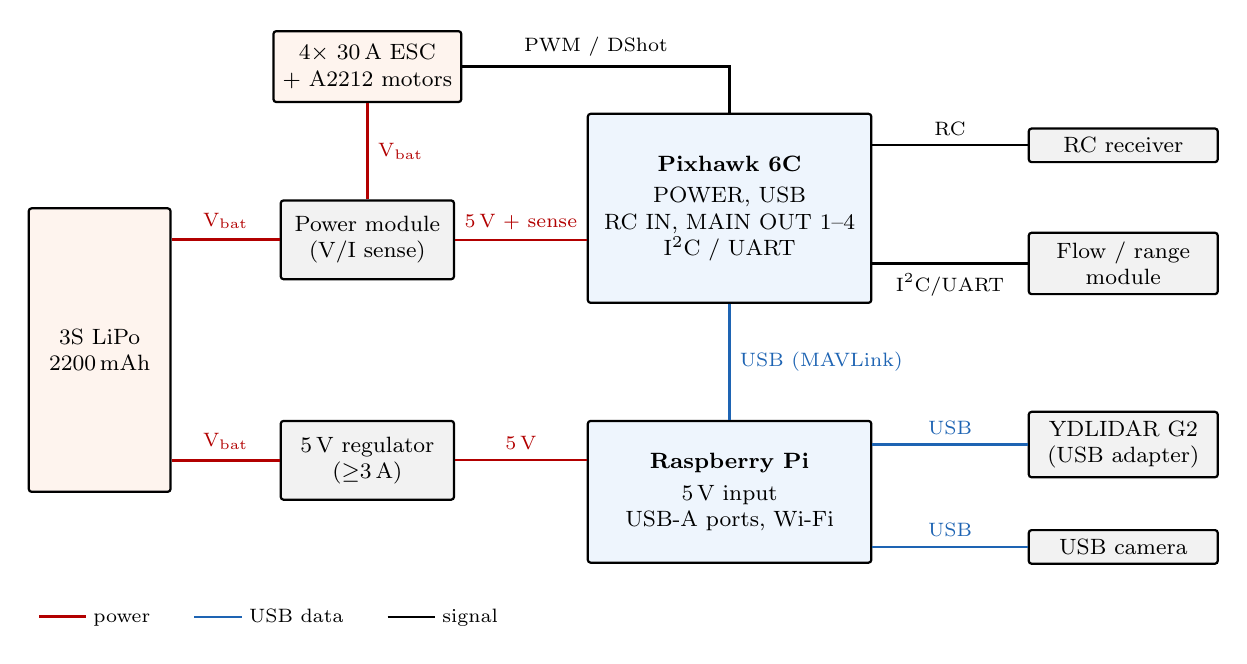
\begin{tikzpicture}[x=1cm, y=1cm, font=\footnotesize,
    box/.style={draw, thick, align=center, rounded corners=1pt},
    pwr/.style={very thick, red!70!black},
    usb/.style={thick, blk1!80!black},
    sig/.style={thick}]
  \node[box, fill=blk2!8, minimum width=18mm, minimum height=36mm] (bat) at (0,-0.2) {3S LiPo\\2200\,mAh};
  \node[box, fill=softgray, minimum width=22mm, minimum height=10mm] (pm)  at (3.4, 1.2) {Power module\\(V/I sense)};
  \node[box, fill=softgray, minimum width=22mm, minimum height=10mm] (bec) at (3.4,-1.6) {5\,V regulator\\($\ge$\SI{3}{\ampere})};
  \node[box, fill=blk2!8, minimum width=22mm, minimum height=9mm]  (esc) at (3.4, 3.4) {4$\times$ 30\,A ESC\\+ A2212 motors};
  \node[box, fill=blk1!8, minimum width=36mm, minimum height=24mm] (fmu) at (8.0, 1.6)
       {\textbf{Pixhawk 6C}\\[2pt]POWER, USB\\RC IN, MAIN OUT 1--4\\I\textsuperscript{2}C / UART};
  \node[box, fill=blk1!8, minimum width=36mm, minimum height=18mm] (pi) at (8.0,-2.0)
       {\textbf{Raspberry Pi}\\[2pt]5\,V input\\USB-A ports, Wi-Fi};
  \node[box, fill=softgray, minimum width=24mm] (rx)    at (13.0, 2.4) {RC receiver};
  \node[box, fill=softgray, minimum width=24mm] (flow)  at (13.0, 0.9) {Flow / range\\module};
  \node[box, fill=softgray, minimum width=24mm] (lidar) at (13.0,-1.4) {YDLIDAR G2\\(USB adapter)};
  \node[box, fill=softgray, minimum width=24mm] (cam)   at (13.0,-2.7) {USB camera};

  \draw[pwr] (bat.east |- pm) -- node[above,font=\scriptsize]{V\textsubscript{bat}} (pm.west);
  \draw[pwr] (bat.east |- bec) -- node[above,font=\scriptsize]{V\textsubscript{bat}} (bec.west);
  \draw[pwr] (pm.north) -- node[right,font=\scriptsize]{V\textsubscript{bat}} (esc.south);
  \draw[pwr, thick] (pm.east) -- node[above,font=\scriptsize]{5\,V + sense} (fmu.west |- pm.east);
  \draw[pwr, thick] (bec.east) -- node[above,font=\scriptsize]{5\,V} (pi.west |- bec.east);
  \draw[sig] (fmu.north) |- node[pos=0.75,above,font=\scriptsize]{PWM / DShot} (esc.east);
  \draw[sig] (rx.west) -- node[above,font=\scriptsize]{RC} (fmu.east |- rx.west);
  \draw[sig] (flow.west) -- node[below,font=\scriptsize]{I\textsuperscript{2}C/UART} (fmu.east |- flow.west);
  \draw[usb] (fmu.south) -- node[right,font=\scriptsize,align=left]{USB (MAVLink)} (pi.north);
  \draw[usb] (lidar.west) -- node[above,font=\scriptsize]{USB} (pi.east |- lidar.west);
  \draw[usb] (cam.west) -- node[above,font=\scriptsize]{USB} (pi.east |- cam.west);

  \node[anchor=west, font=\scriptsize] at (-0.9,-3.6)
    {\textcolor{red!70!black}{\rule[0.5ex]{6mm}{1.4pt}}~power\qquad
     \textcolor{blk1!80!black}{\rule[0.5ex]{6mm}{1pt}}~USB data\qquad
     \rule[0.5ex]{6mm}{0.8pt}~signal};
\end{tikzpicture}
\caption{Connector-level interconnection schematic of the prototype. A Raspberry Pi with USB
peripherals should be supplied from a regulator rated at least \SI{3}{\ampere}, not
from the autopilot's servo rail.}
\label{fig:wiring}
\end{figure}

\subsection{Network interface}

Each data stream uses its own transport and port (\cref{tab:ports}). Only one process
may bind a given laptop port, so the stand-alone (ROS-free) laptop tools are used
\emph{instead of}, not alongside, the ROS stack.

\begin{table}[H]
\centering\small
\caption{Pi--laptop interface (from \code{docs/REFERENCE.md} and the source).}
\label{tab:ports}
\begin{tabularx}{\textwidth}{l l l >{\raggedright\arraybackslash}p{3.3cm} L}
\toprule
\textbf{Stream} & \textbf{Dir.} & \textbf{Transport} & \textbf{Encoding / QoS} & \textbf{Endpoints $\rightarrow$ ROS topic} \\
\midrule
Telemetry & Pi$\rightarrow$L & UDP 14551 & JSON $\le$\SI{1400}{B}, DSCP CS6 & \code{telemetry_streamer.py} $\rightarrow$ \code{mavlink_to_ros2_bridge} $\rightarrow$ \topic{/odom}, TF \\
Raw MAVLink & Pi$\rightarrow$L & UDP 14550 & MAVLink v2 & monitoring only (e.g.\ QGroundControl) \\
LiDAR & Pi$\rightarrow$L & UDP 14552 & binary \SI{1094}{B}, DSCP CS6 & \code{lidar_udp_streamer.py} $\rightarrow$ \code{lidar_udp_receiver} $\rightarrow$ \topic{/scan} \\
Camera & Pi$\rightarrow$L & TCP 5000 & JPEG + JSON header, DSCP AF41 & \code{camera_streamer.py} $\rightarrow$ \code{camera_tcp_receiver} $\rightarrow$ \topic{/camera/image_raw} \\
Velocity & L$\rightarrow$Pi & UDP 14553 & JSON, DSCP CS6 & \code{mavlink_cmd_bridge} $\rightarrow$ \code{mavlink_cmd_listener.py} \\
Mode/arm & L$\rightarrow$Pi & UDP 14552 & JSON & \code{mavlink_cmd_bridge} $\rightarrow$ \code{telemetry_streamer.py} \\
\bottomrule
\end{tabularx}
\end{table}

\subsection{Software architecture}

\paragraph{Airborne processes} \code{start_streams.py} is the single entry point on
the Pi. It launches and supervises three child processes (telemetry, LiDAR, camera),
restarts any that exit with back-off, and optionally (\code{--nav-cmds}) runs the
velocity listener \emph{inside} the telemetry process so that it shares that process's
MAVLink connection; only one process can own the autopilot's serial port. On start it also disables Wi-Fi power saving on the interface that routes
to the laptop (re-checked every \SI{30}{\second}) and adds the laptop as the preferred
\code{chrony} time source. Both changes are reverted on exit.

\paragraph{Ground ROS~2 packages} \Cref{tab:packages} lists the workspace packages. A
single launch file, \code{navigation_real.launch.py}, starts the bridge nodes, static
transforms, Nav2, perception, the 3D mapper, the metrics monitor and RViz.

\begin{table}[H]
\centering\small
\caption{ROS~2 workspace packages.}
\label{tab:packages}
\begin{tabularx}{\textwidth}{l L}
\toprule
\textbf{Package} & \textbf{Role} \\
\midrule
\code{gps_denied_bridge} & Pi$\leftrightarrow$ROS bridge: telemetry$\rightarrow$\topic{/odom}+TF, LiDAR$\rightarrow$\topic{/scan}, camera, \topic{/cmd_vel}$\rightarrow$Pi, health metrics, 3D voxel mapping \\
\code{x500_navigation} & Nav2 parameter sets (real, office, Baylands), SLAM configs, launch files, RViz layouts, drone behaviour tree, office world generator \\
\code{quadcopter_perception} & Hybrid YOLO + SAM segmentation node and ROS-independent core, unit tests \\
\code{x500_px4_bridge} & Simulation: Nav2 $\rightarrow$ PX4 OFFBOARD bridge with LiDAR safety filter; Gazebo Harmonic transport bridge; TF broadcaster \\
\code{quadcopter_bringup} & Simulation bring-up and keyboard/GUI teleoperation \\
\code{quadcopter_localization}, \code{quadcopter_mapping} & Early work (VO$\rightarrow$PX4 parameters, frame utilities; mapping stub) \\
\code{m-explore-ros2}, \code{px4_msgs} & Third-party: frontier exploration \cite{hoerner2016mapmerge}, PX4 message definitions \\
\bottomrule
\end{tabularx}
\end{table}

\subsection{Coordinate frames}
\label{sec:frames}

ROS uses an East--North--Up (ENU) world frame and a Forward--Left--Up (FLU) body
frame \cite{rep103,rep105}. ArduPilot and PX4 use North--East--Down (NED) and
Forward--Right--Down (FRD). All conversions take place at the bridge boundary, so the
rest of the stack sees a single convention (\cref{fig:tf}).

\begin{figure}[H]
\centering
\begin{tikzpicture}[node distance=4mm and 9mm, font=\footnotesize]
  \node[blk, fill=softgray] (map) {\code{map}};
  \node[blk, fill=softgray, right=13mm of map] (odom) {\code{odom}};
  \node[blk, fill=blk1!10, right=of odom] (base) {\code{base_link}};
  \node[blk, fill=blk3!10, above right=1mm and 9mm of base] (laser) {\code{laser_frame}};
  \node[blk, fill=blk3!10, below right=1mm and 9mm of base] (cam) {\code{camera_frame}};
  \draw[arr, dashed] (map) -- node[lbl,above]{SLAM} (odom);
  \draw[arr] (odom) -- node[lbl,above]{bridge} (base);
  \draw[arr] (base) -- node[lbl,above,sloped]{static} (laser);
  \draw[arr] (base) -- node[lbl,below,sloped]{static} (cam);
\end{tikzpicture}
\caption{Transform tree on the real vehicle. \code{odom}$\rightarrow$\code{base_link}
is broadcast by \code{mavlink_to_ros2_bridge}. Sensor mounts are static transforms.
In the real configuration Nav2 operates in \code{odom} (rolling costmaps, no global map).
The simulation adds \code{map}$\rightarrow$\code{odom} from SLAM~Toolbox and a
\code{base_footprint} frame for 2D planning.}
\label{fig:tf}
\end{figure}

%% ---------------------------------------------------------------------
\section{Design methodology and technical justification}
\label{sec:design}

\subsection{Trade study of GPS-denied navigation modalities}
\label{sec:design-trade}

Fifteen candidate approaches were screened (\cref{tab:solutions}) on drift (percent
of distance travelled), power, mass, update rate, range and cost in Indian rupees.
The values are concept-phase, literature-typical estimates
(\code{docs/ANALYSIS_SOLUTIONS.md}), not measurements. \Cref{fig:trade} summarises
them; further views are in \cref{app:trade}.

\begin{table}[H]
\centering\scriptsize
\caption{Screening data for the 15 modalities (mid-range values; ranges in
\code{docs/ANALYSIS_SOLUTIONS.md}).}
\label{tab:solutions}
\renewcommand{\arraystretch}{1.1}
\begin{tabularx}{\textwidth}{r L r r r r r}
\toprule
\# & \textbf{Modality} & \textbf{Drift (\%)} & \textbf{Power (W)} & \textbf{Mass (g)} & \textbf{Rate (Hz)} & \textbf{Cost (kINR)} \\
\midrule
1 & 2D LiDAR + optical flow & 1.4 & 7.0 & 150 & 75 & 12.5 \\
2 & Stereo camera V-SLAM (Pi~5) & 0.3 & 10.5 & 85 & 40 & 18.0 \\
3 & 2D LiDAR + monocular RGB & 1.5 & 8.0 & 140 & 35 & 15.5 \\
4 & Event camera odometry & 1.4 & 5.5 & 42.5 & 750 & 45.0 \\
5 & Visual SLAM & 0.3 & 17.5 & 85 & 40 & 12.0 \\
6 & Ultrasonic array & 2.5 & 1.25 & 27.5 & 30 & 16.5 \\
7 & Optical flow + rangefinder & 3.5 & 2.0 & 25 & 75 & 7.75 \\
8 & ArUco / fiducial tags & abs.\ $\pm$2\,cm & 2.0 & 20 & 20 & 5.0 \\
9 & Three RGB cameras (Pi~5) & 0.65 & 13.0 & 105 & 22.5 & 14.0 \\
10 & Depth camera (Pi~5) & 1.0 & 10.0 & 70 & 22.5 & 26.0 \\
11 & 3D LiDAR SLAM (Pi~5) & 0.125 & 22.5 & 375 & 15 & 425 \\
12 & FMCW mmWave radar & 2.0 & 7.0 & 120 & 35 & 77.5 \\
13 & UWB beacons & abs.\ $\pm$2\,cm & 2.0 & 20 & 75 & 30.0 \\
14 & Magnetic anomaly (MAGNAV) & 0.6 & 3.5 & 70 & 20 & 40.0 \\
15 & Terrain matching (TERCOM) & 0.45 & 10.0 & 225 & 12.5 & 235 \\
\bottomrule
\end{tabularx}
\end{table}

\begin{figure}[t]
\centering
\begin{subfigure}[t]{0.49\textwidth}
  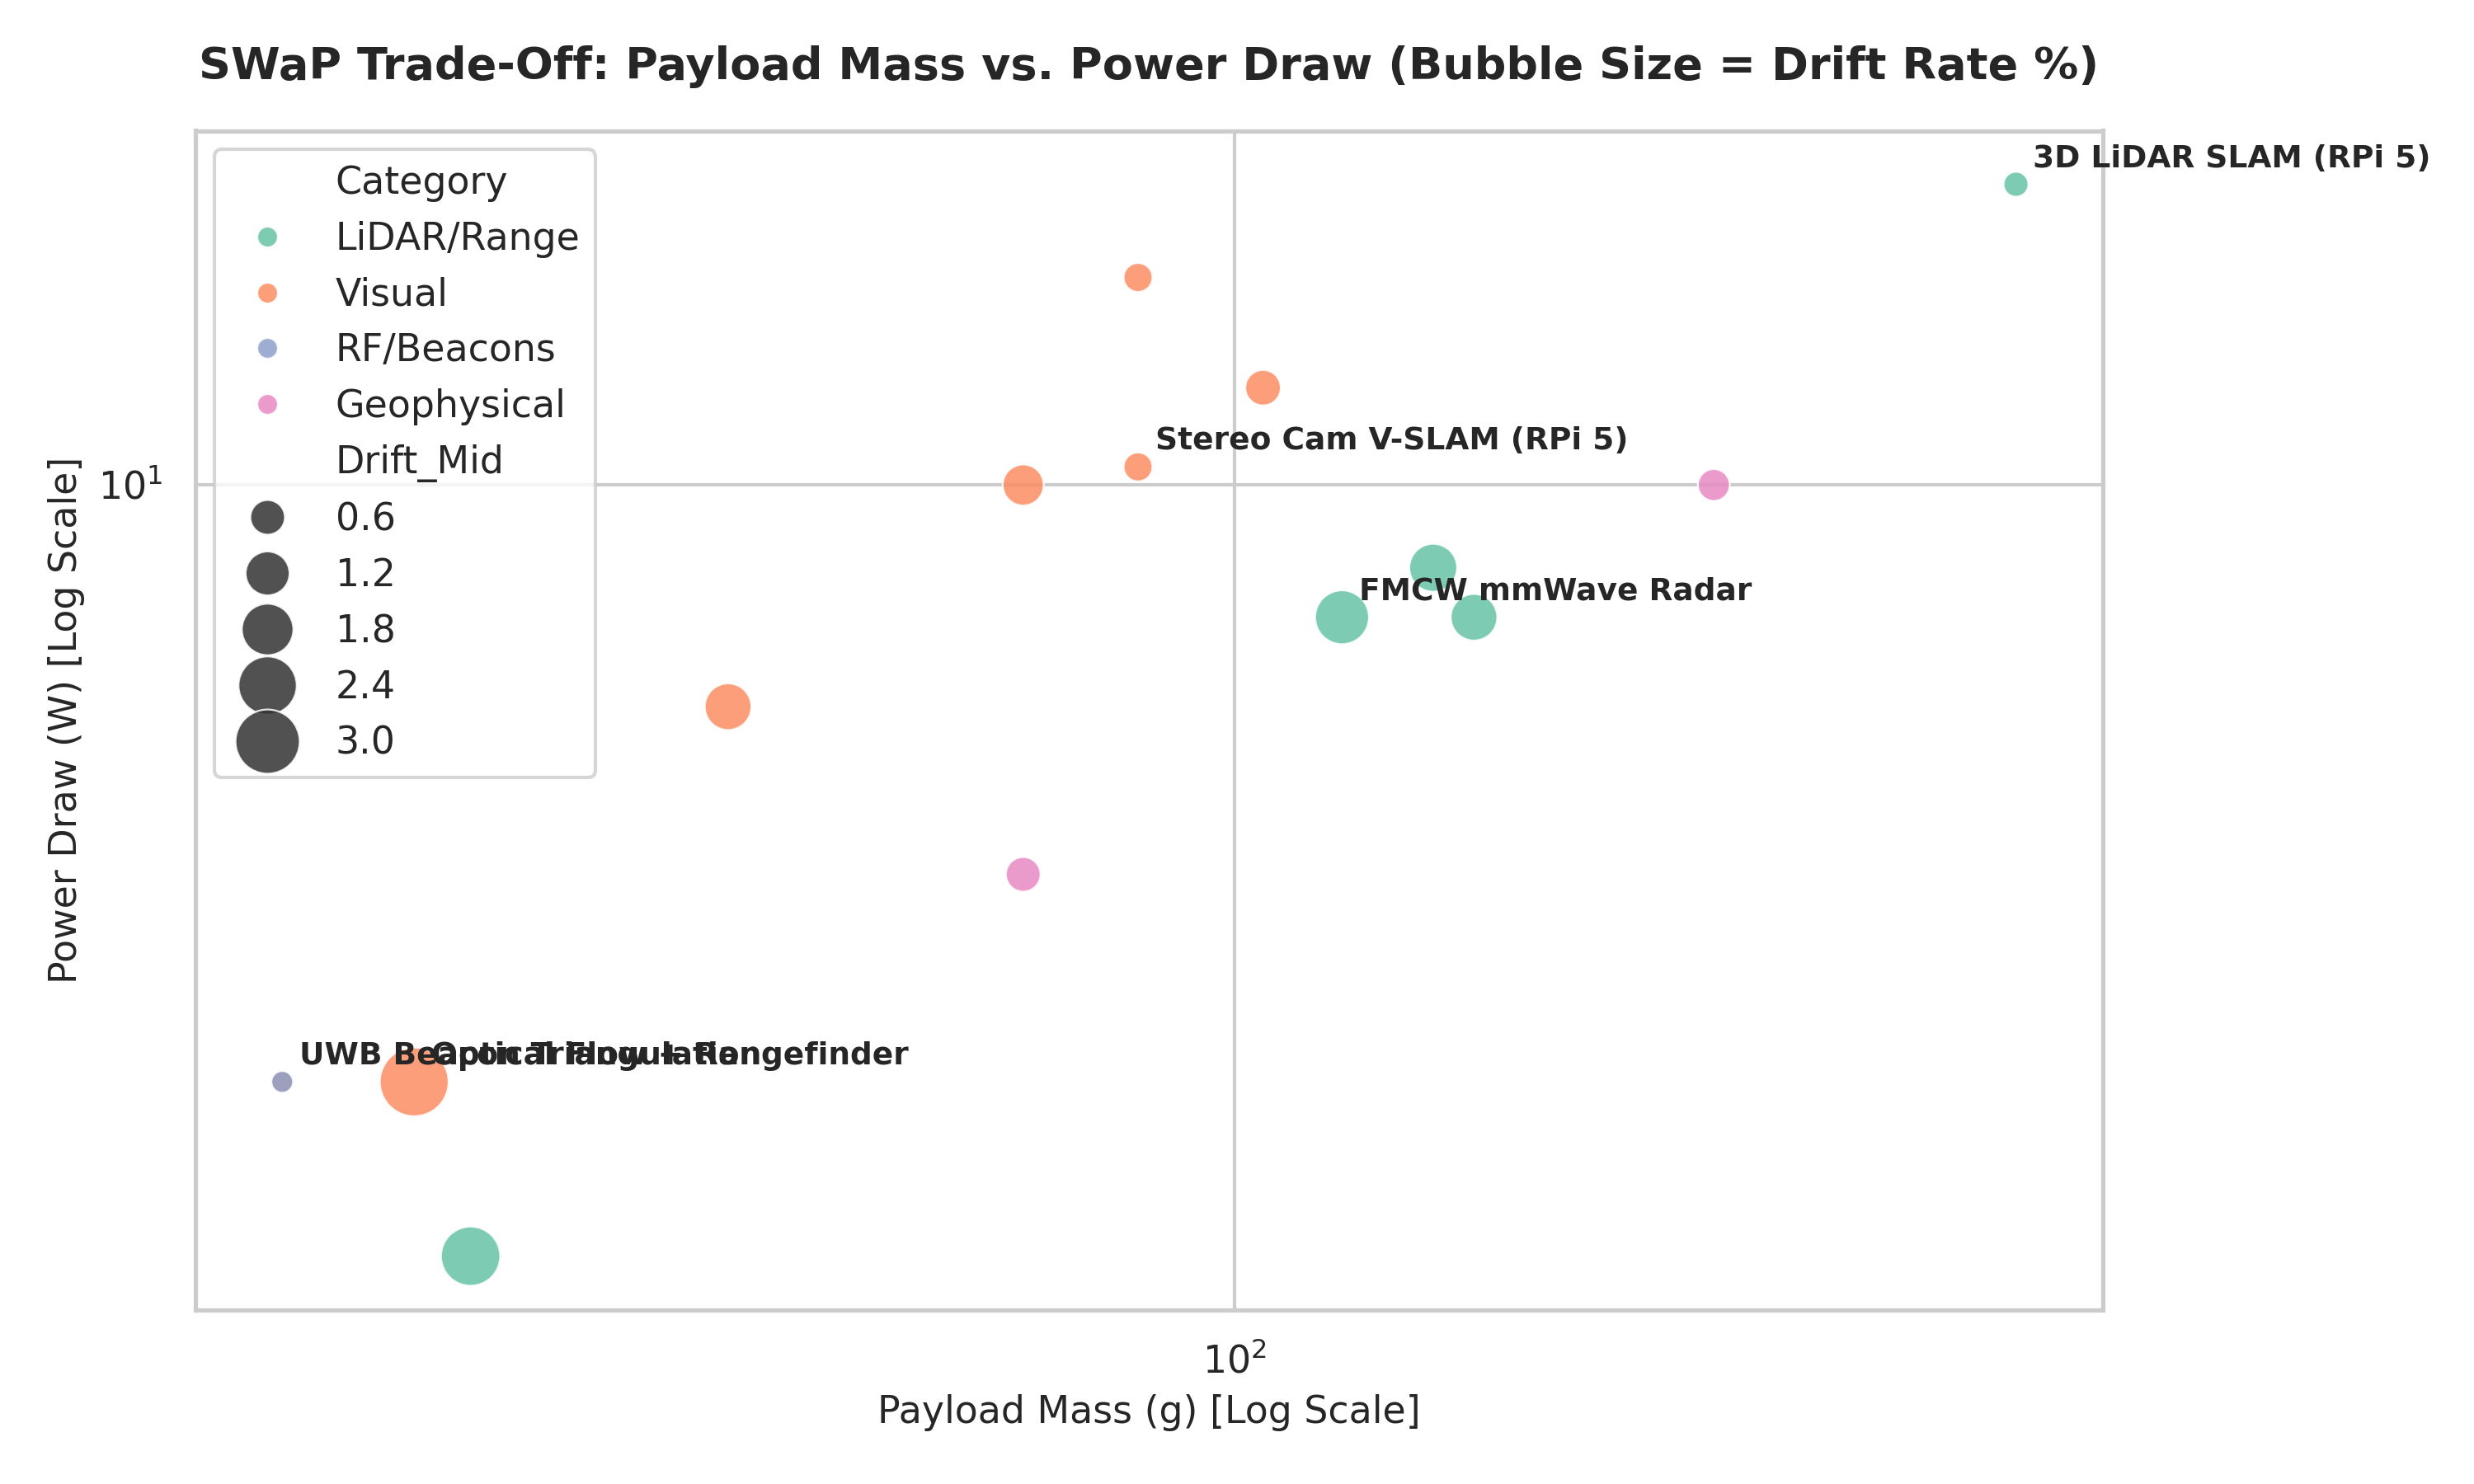
\includegraphics[width=\linewidth]{1_swap_tradeoff.png}
  \caption{SWaP trade-off (bubble size = drift).}
\end{subfigure}\hfill
\begin{subfigure}[t]{0.49\textwidth}
  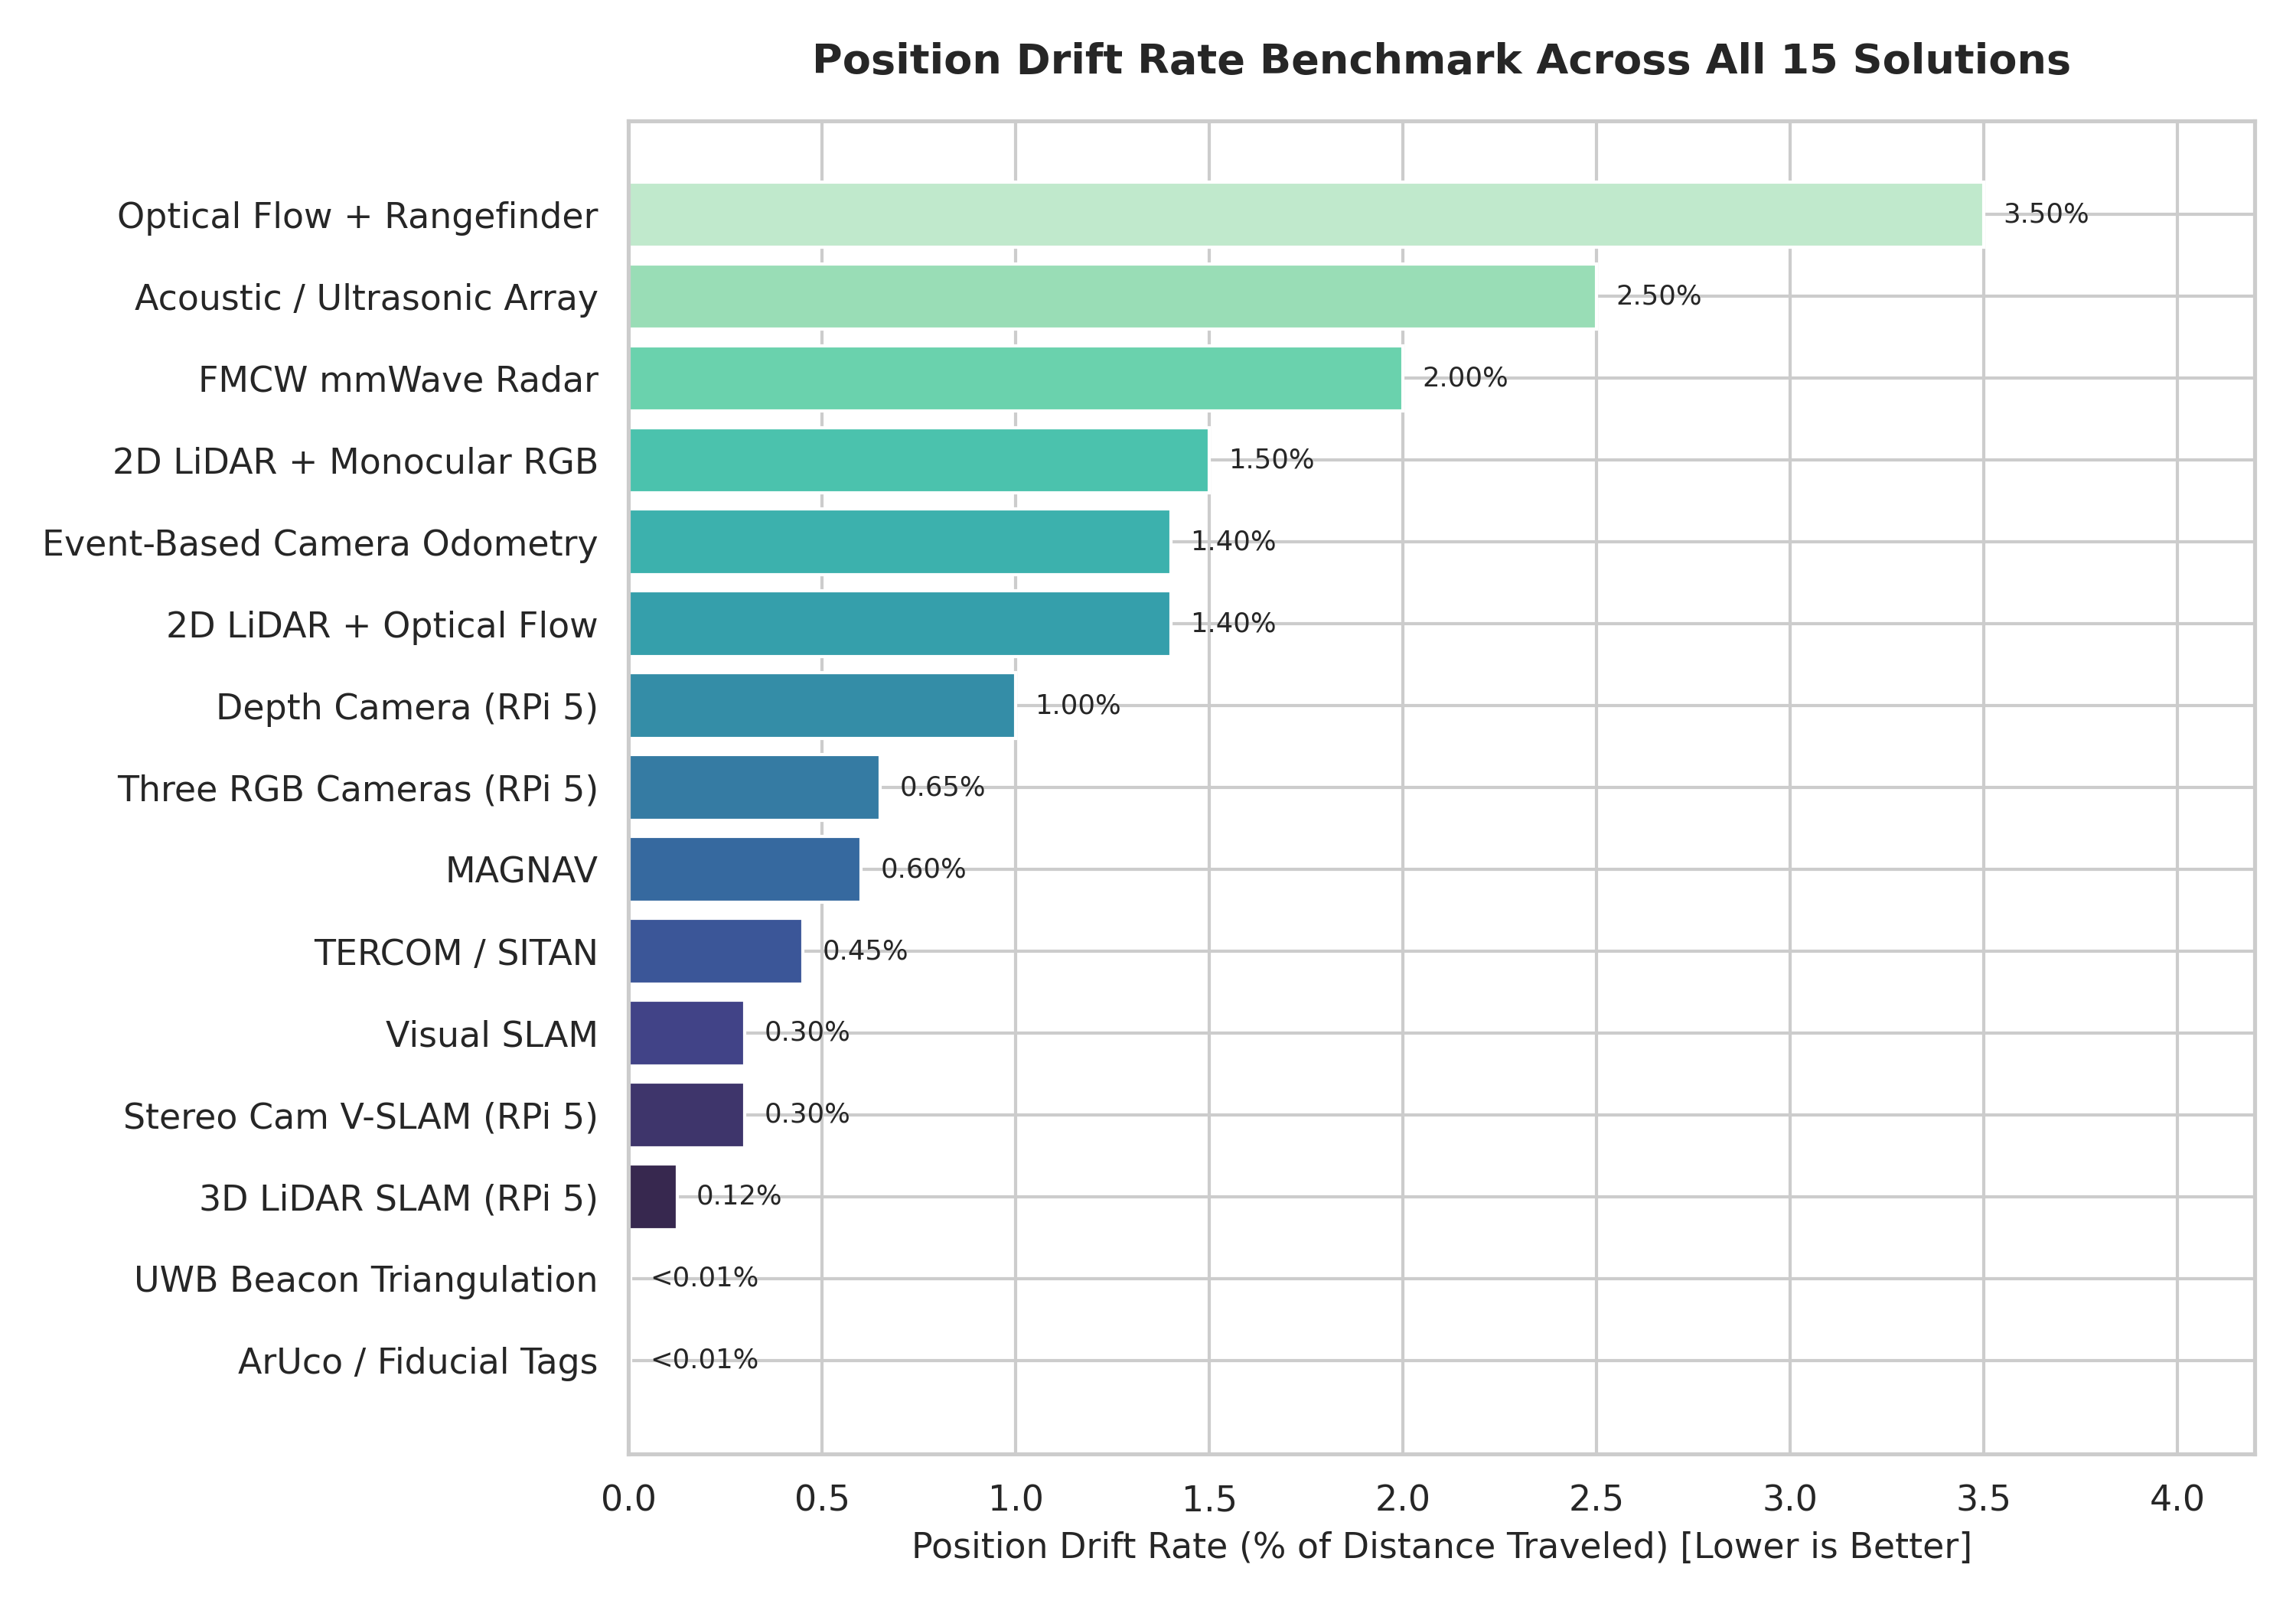
\includegraphics[width=\linewidth]{2_drift_rate_comparison.png}
  \caption{Drift rate ranking.}
\end{subfigure}

\vspace{2mm}
\begin{subfigure}[t]{0.49\textwidth}
  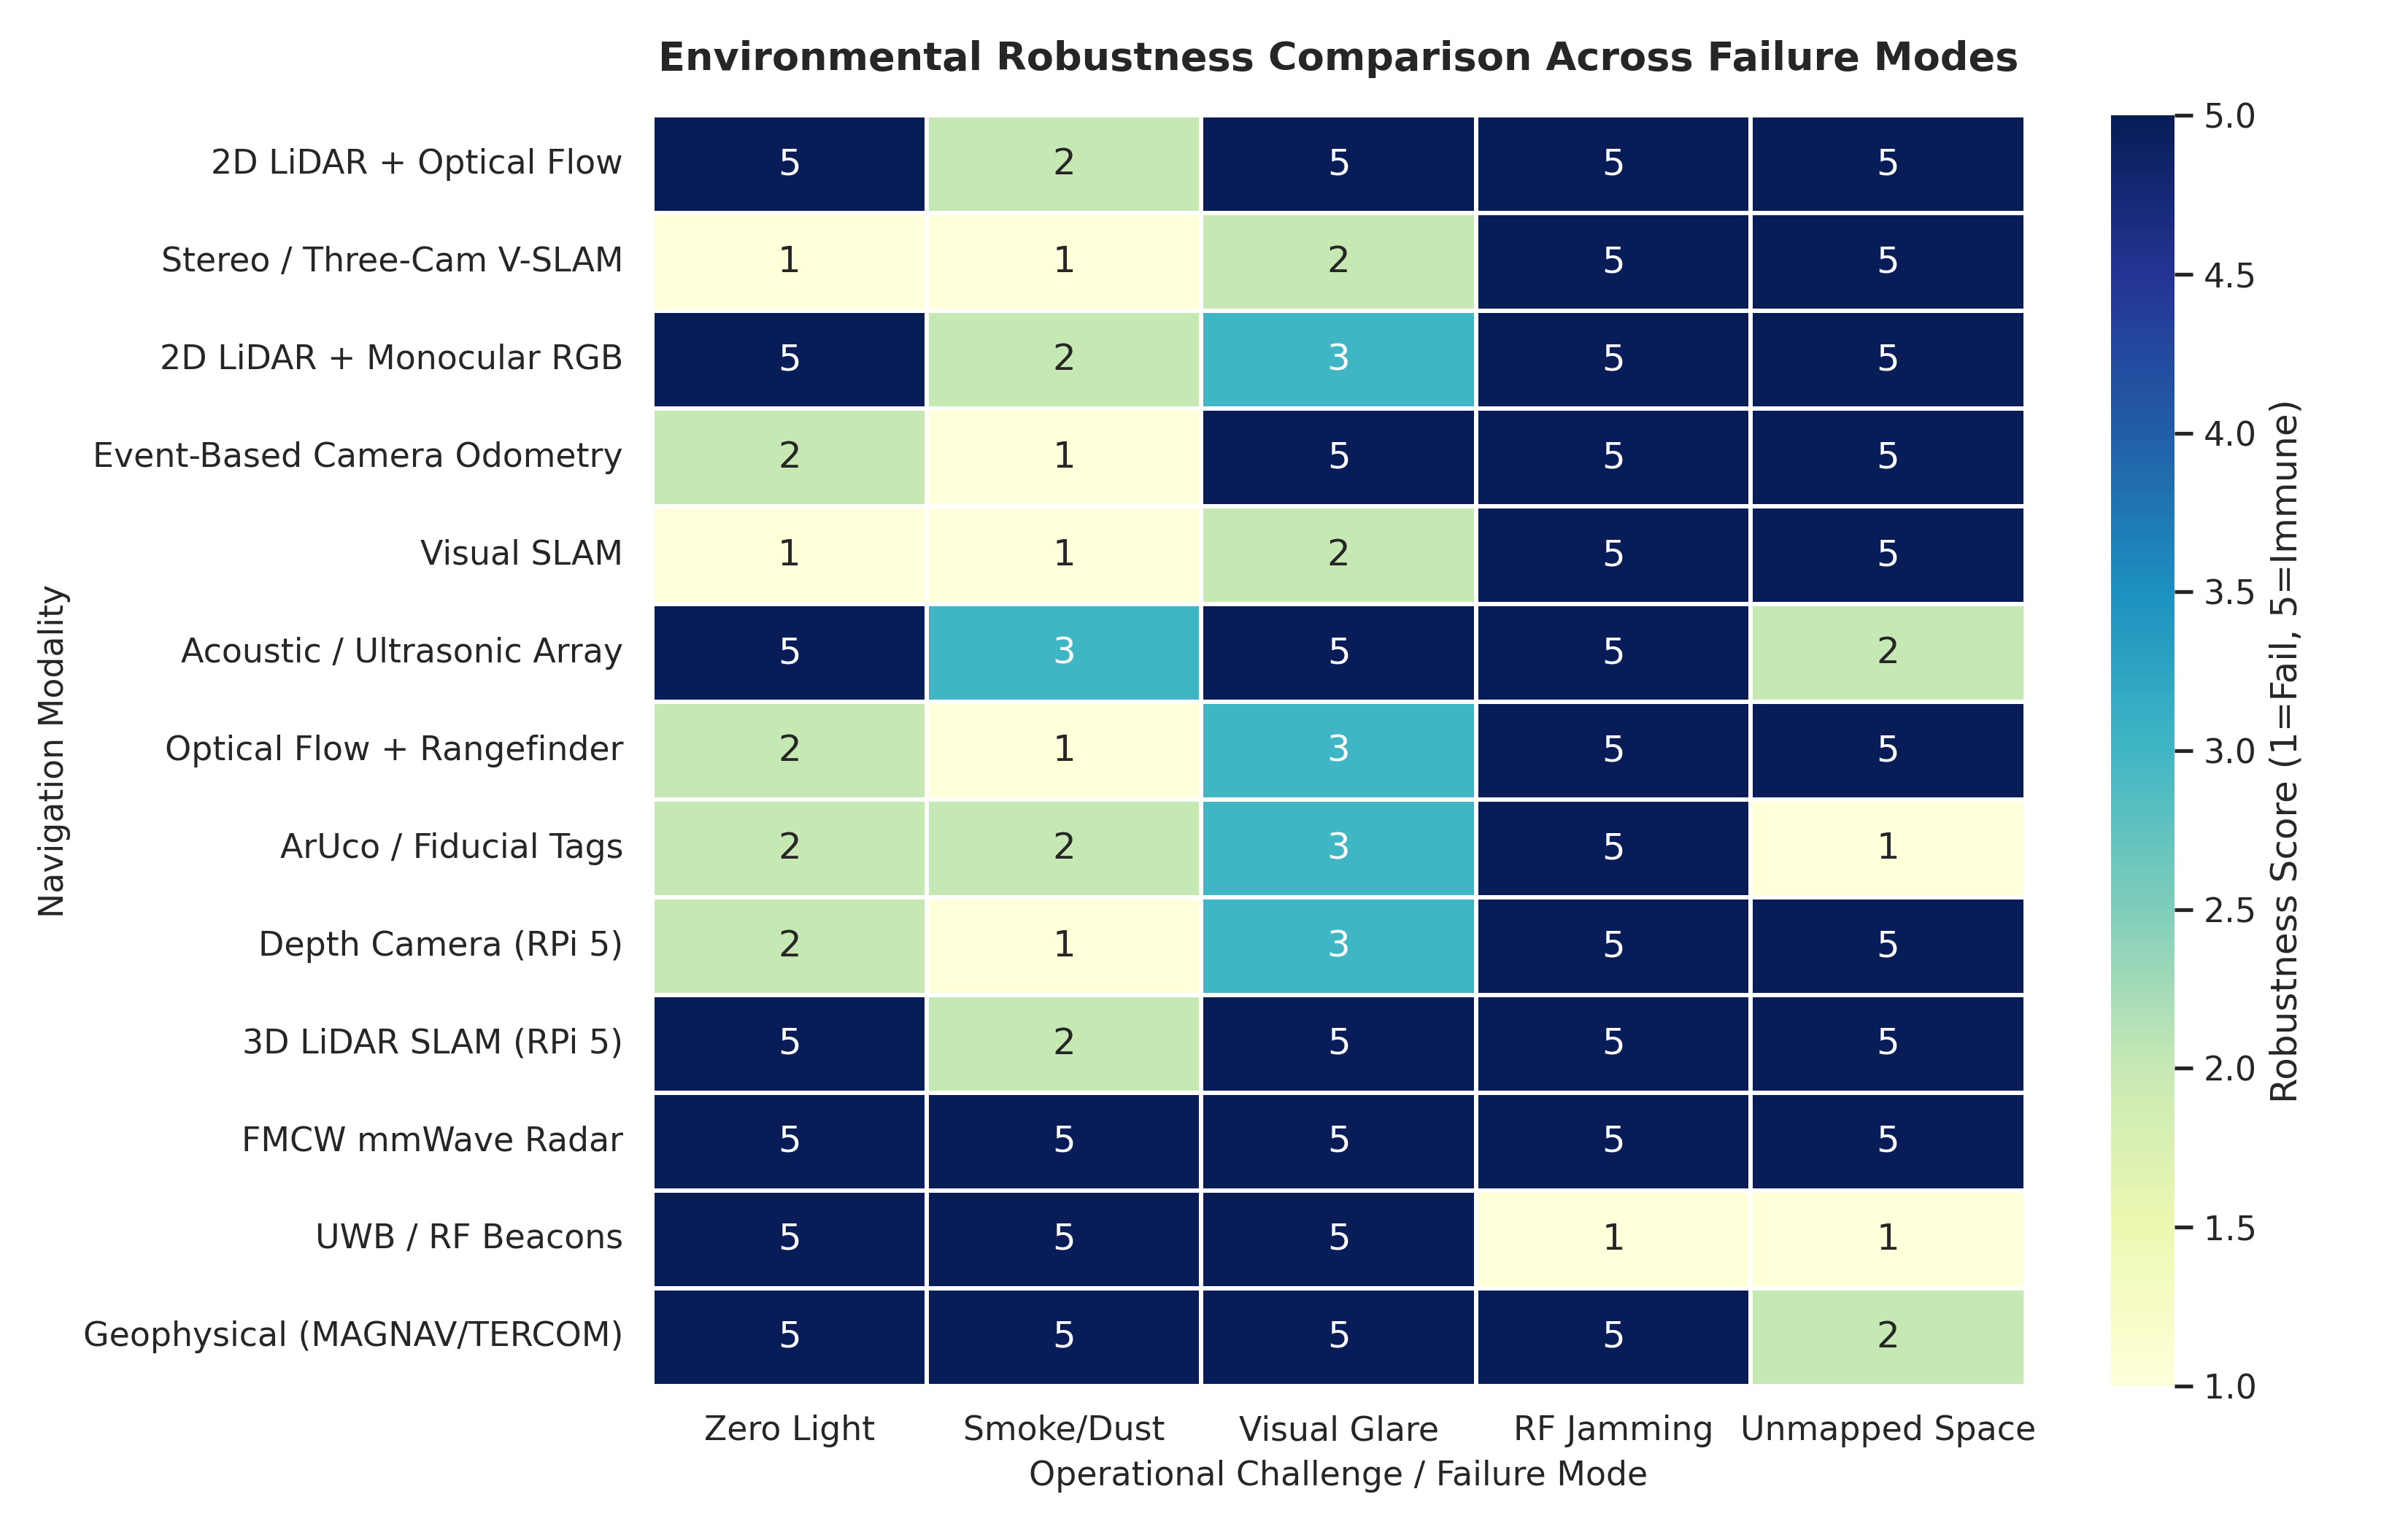
\includegraphics[width=\linewidth]{4_robustness_heatmap.png}
  \caption{Environmental robustness (1 = fails, 5 = unaffected).}
\end{subfigure}\hfill
\begin{subfigure}[t]{0.49\textwidth}
  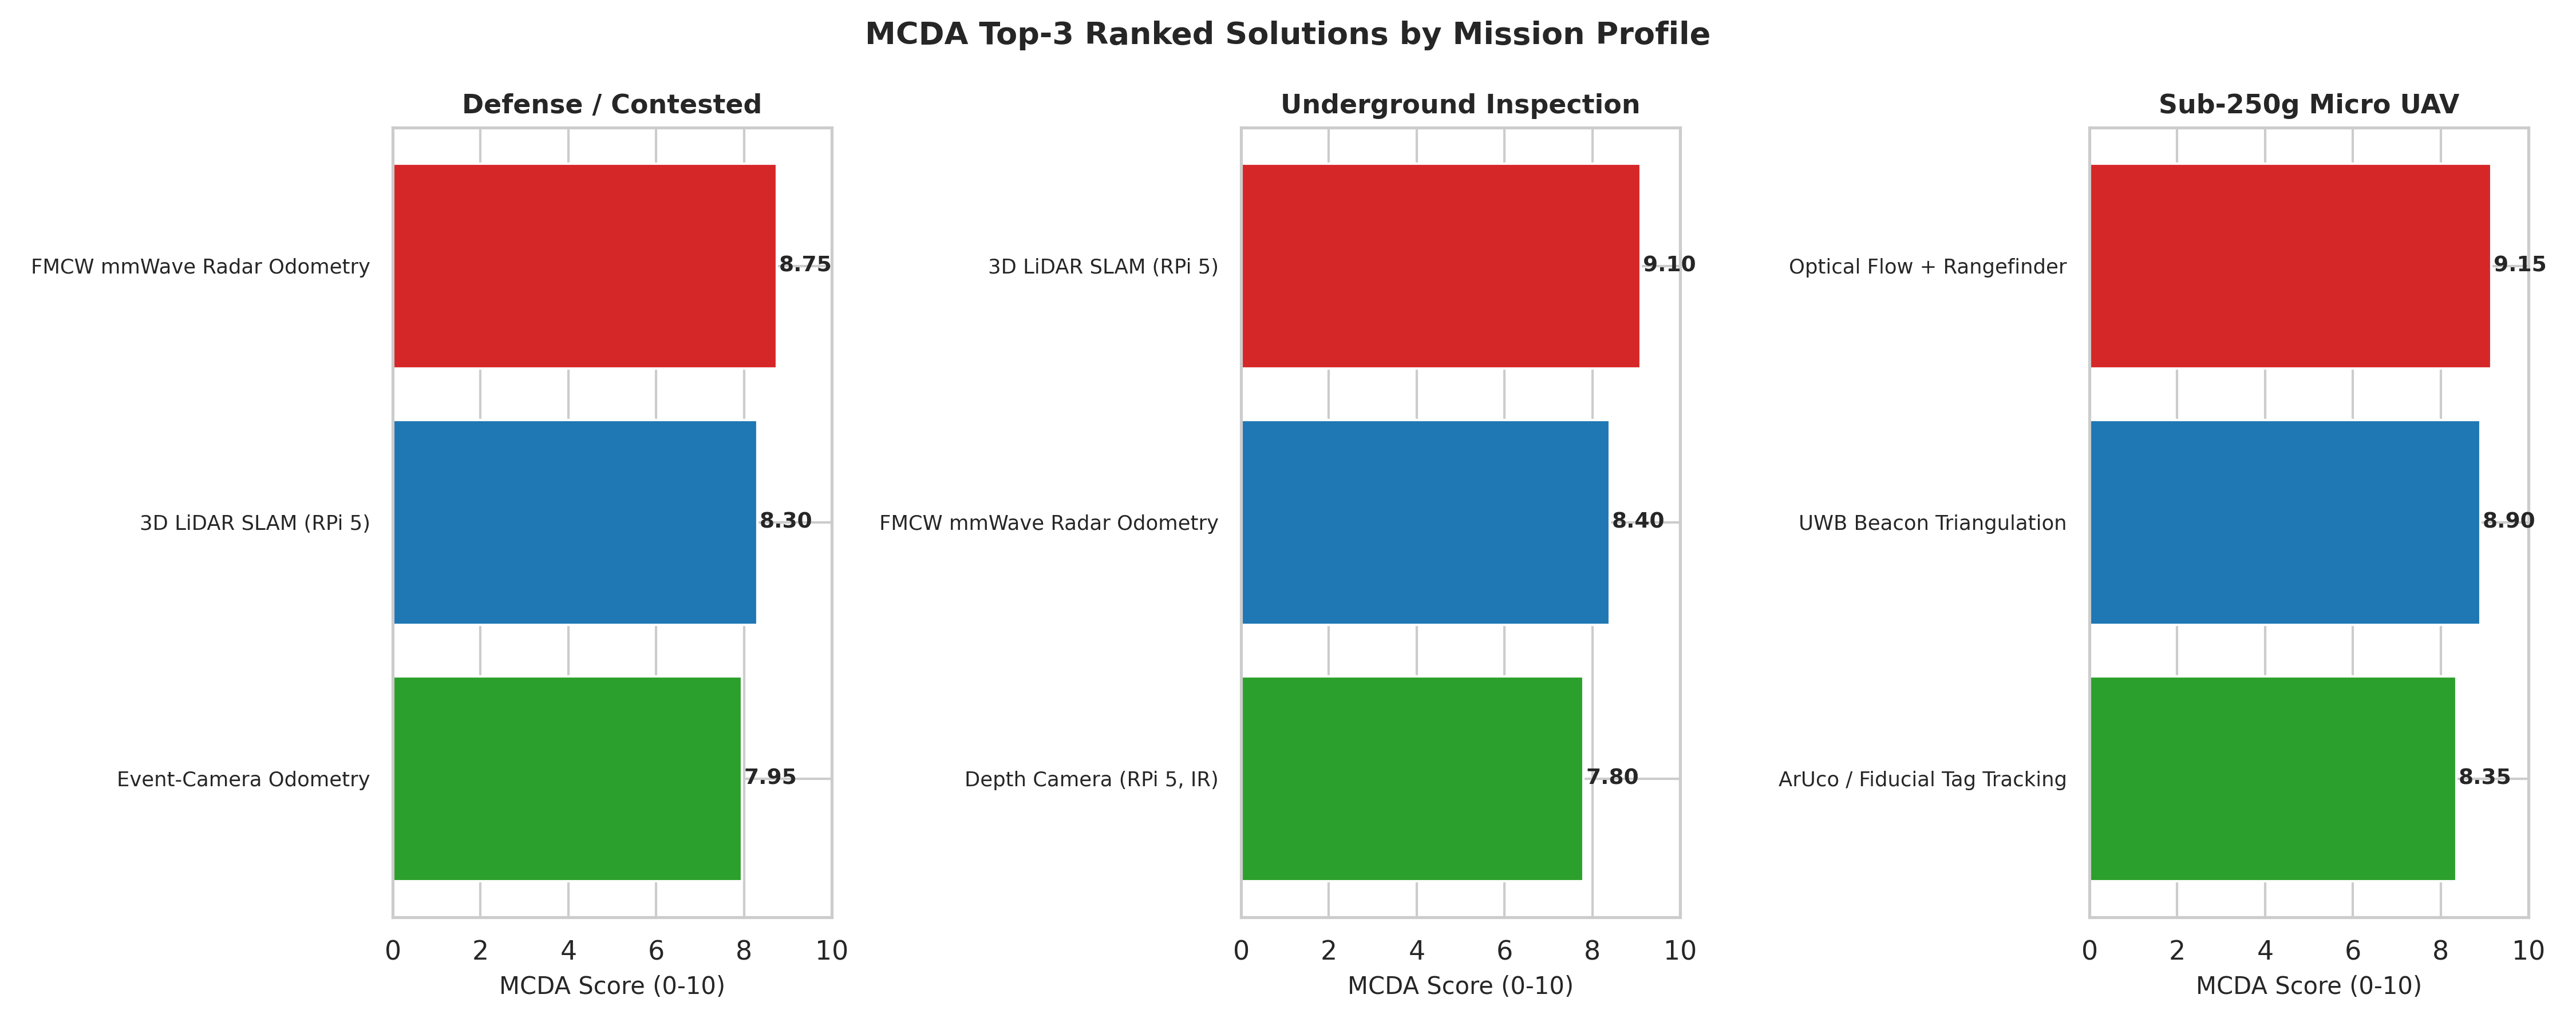
\includegraphics[width=\linewidth]{12_mcda_scenarios.png}
  \caption{Top-3 weighted scores per mission.}
\end{subfigure}
\caption{Concept-phase trade study. Values are screening estimates, not measurements.}
\label{fig:trade}
\end{figure}


The lowest-drift options are either expensive (3D LiDAR SLAM, about \INR{4.25} lakh;
terrain matching) or need infrastructure (UWB beacons, fiducial tags). Among
self-contained options under \INR{20{,}000}, 2D LiDAR with optical flow has the highest
robustness total (22 of 25), exceeded only by mmWave radar (25).

\paragraph{Robustness} Each modality was scored from 1 (fails) to 5 (unaffected)
against darkness, smoke/dust, glare, RF jamming and unmapped space (\cref{fig:trade}c).
Visual methods fail in darkness and smoke, beacons under jamming and in unprepared
areas; LiDAR and radar are the only self-contained options that tolerate darkness.

\paragraph{Multi-criteria decision analysis} For a mission profile $m$ with criteria
weights $w_{m,j}$ ($\sum_j w_{m,j}=1$) and per-criterion ratings $r_{i,j}\in[1,10]$,
the score of solution $i$ is the weighted sum \cite{triantaphyllou2000mcdm}
\begin{equation}
  S_{i,m} = \sum_{j} w_{m,j}\, r_{i,j}.
\end{equation}
\Cref{tab:mcda} gives the weights and the three best-ranked modalities per mission.

\begin{table}[H]
\centering\small
\caption{Weighted-sum ranking for three mission profiles (scores out of 10).}
\label{tab:mcda}
\begin{tabularx}{\textwidth}{p{2.5cm} L p{2.3cm} p{2.3cm} p{2.3cm}}
\toprule
\textbf{Mission} & \textbf{Weights} & \textbf{1st} & \textbf{2nd} & \textbf{3rd} \\
\midrule
Defence / jammed airspace & jamming 30\%, dark/smoke 25\%, SWaP 25\%, precision 20\% & mmWave radar (8.75) & 3D LiDAR SLAM (8.30) & Event camera (7.95) \\
Underground inspection & darkness 35\%, precision 25\%, SWaP 20\%, unknown area 20\% & 3D LiDAR SLAM (9.10) & mmWave radar (8.40) & Depth camera, IR (7.80) \\
Micro-UAV ($<$\SI{250}{\gram}) & mass 40\%, power 30\%, rate 15\%, precision 15\% & Optical flow + rangefinder (9.15) & UWB beacons (8.90) & ArUco markers (8.35) \\
\bottomrule
\end{tabularx}
\end{table}

\paragraph{Design decisions} Two configurations followed from the study.
\begin{enumerate}[leftmargin=*,itemsep=1pt]
  \item \emph{Design target: stereo V-SLAM on a Raspberry Pi~5 (modality~2).}
    Sub-percent drift at under \SI{100}{\gram} and about \SI{10}{\watt}, passive, no
    infrastructure, within the \INR{45.7}k budget and \SI{500}{\gram} payload. Its
    weakness in darkness and textureless scenes is to be covered by flow/range sensing.
  \item \emph{Current prototype: 2D LiDAR + optical flow + monocular RGB (modalities
    1 and 3).} The sensors already on the vehicle. They work in darkness, give Nav2
    metric obstacle geometry immediately and leave the camera free for perception, at a
    predicted 1.4--1.5\% drift. They serve as the platform for developing the link,
    planning and safety layers that the design target will reuse.
\end{enumerate}

\subsection{Partitioning between autopilot, companion and ground computer}

Responsibilities were assigned by time scale and criticality:
\begin{itemize}[leftmargin=*,itemsep=1pt]
  \item \textbf{Autopilot} (\si{\kilo\hertz} loops): attitude, rate and thrust control,
    EKF3, motor output, RC handling, failsafes. These never depend on the companion.
  \item \textbf{Companion} (\SIrange{7}{30}{\hertz}): I/O only. It reads sensors,
    timestamps at the source, encodes compactly, and forwards velocity setpoints with
    local safety gating. Keeping it free of ROS and heavy computation keeps it
    deterministic and leaves the Pi~5 free to take on onboard processing later.
  \item \textbf{Ground} (\SIrange{1}{30}{\hertz}): odometry reconstruction, costmaps,
    planning, segmentation, visualisation and metrics.
\end{itemize}

\subsection{Link design for low latency}
\label{sec:design-link}

Latency is lost in sensor batching, companion queues and the Wi-Fi medium; each
was addressed in code.

\paragraph{Single-datagram encodings} An IP datagram larger than the path MTU is
fragmented, and losing any fragment loses the whole datagram. On a lossy wireless link
the delivery probability of an $n$-fragment message falls to
\begin{equation}
  P_{\text{deliver}} = (1-p)^{n},
  \label{eq:frag}
\end{equation}
for fragment loss probability $p$. The original JSON LiDAR scan was about \SI{4}{kB}
($n{=}3$). The binary encoding (\cref{fig:packets}) has length
\begin{equation}
  L_{\text{scan}} = \underbrace{4}_{\text{magic}} + \underbrace{8}_{t_\text{capture}} +
  \underbrace{2}_{N} + 2N + N = 14 + 3N\ \text{bytes},
\end{equation}
which for $N{=}360$ is \SI{1094}{B}, a single datagram. Telemetry snapshots of
\SIrange{1.6}{1.8}{kB} are cut to at most \SI{1400}{B} by always sending the
navigation fields and rotating five bulky, slowly-changing fields
(\code{global_position}, \code{ekf_status}, \code{vibration}, \code{rc_channels},
\code{statustexts}) round-robin across packets.
\Cref{fig:delivery} plots \cref{eq:frag} for both encodings.

\begin{figure}[H]
\centering
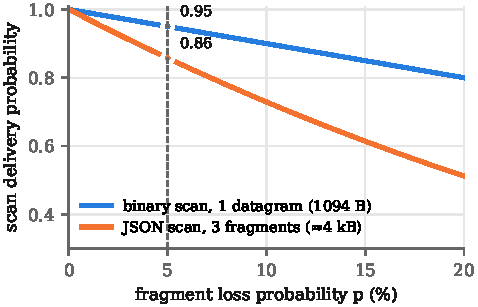
\includegraphics[width=0.5\textwidth]{packet_delivery.pdf}
\caption{Delivery probability of one LiDAR scan against per-fragment loss
(\cref{eq:frag}). At 5\% loss the single-datagram encoding arrives 95\% of the time,
against 86\% for the three-fragment JSON scan.}
\label{fig:delivery}
\end{figure}

\begin{figure}[H]
\centering
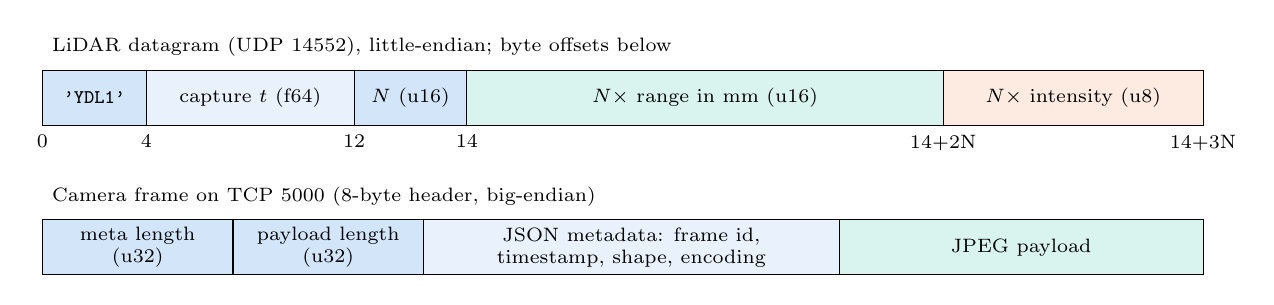
\begin{tikzpicture}[font=\scriptsize, x=1.1mm, y=1mm]
  \def\h{7}
  \draw[fill=blk1!20] (0,0)   rectangle (12,\h)  node[midway]{\texttt{'YDL1'}};
  \draw[fill=blk1!10] (12,0)  rectangle (36,\h)  node[midway]{capture $t$ (f64)};
  \draw[fill=blk1!20] (36,0)  rectangle (49,\h)  node[midway]{$N$ (u16)};
  \draw[fill=blk3!15] (49,0)  rectangle (104,\h) node[midway]{$N\times$ range in mm (u16)};
  \draw[fill=blk2!15] (104,0) rectangle (134,\h) node[midway]{$N\times$ intensity (u8)};
  \foreach \x/\l in {0/0,12/4,36/12,49/14,104/{14+2N},134/{14+3N}} \node[below] at (\x,0) {\l};
  \node[anchor=west] at (0,\h+3) {LiDAR datagram (UDP 14552), little-endian; byte offsets below};
  \begin{scope}[yshift=-19mm]
    \draw[fill=blk1!20] (0,0)  rectangle (22,\h)  node[midway, align=center]{meta length\\(u32)};
    \draw[fill=blk1!20] (22,0) rectangle (44,\h)  node[midway, align=center]{payload length\\(u32)};
    \draw[fill=blk1!10] (44,0) rectangle (92,\h)  node[midway, align=center]{JSON metadata: frame id,\\timestamp, shape, encoding};
    \draw[fill=blk3!15] (92,0) rectangle (134,\h) node[midway]{JPEG payload};
    \node[anchor=west] at (0,\h+3) {Camera frame on TCP 5000 (8-byte header, big-endian)};
  \end{scope}
\end{tikzpicture}
\caption{Wire formats of the LiDAR and camera streams.}
\label{fig:packets}
\end{figure}

\paragraph{Event-driven telemetry} ArduPilot's legacy \code{REQUEST_DATA_STREAM} groups
are limited to \SI{10}{\hertz}, which adds up to \SI{100}{\milli\second} of age. The
companion requests the five navigation messages (\code{ATTITUDE},
\code{LOCAL_POSITION_NED}, \code{OPTICAL_FLOW}, \code{RAW_IMU},
\code{DISTANCE_SENSOR}) at \SI{30}{\hertz} through
\code{MAV_CMD_SET_MESSAGE_INTERVAL}. The request is re-issued after the stream
requests, because ArduPilot resets per-message intervals when a group request is
applied. A packet is sent as soon as fresh navigation data arrive, after a
\SI{3}{\milli\second} coalescing window that merges one autopilot burst into one
packet. A \SI{200}{\milli\second} keep-alive covers quiet periods.
\Cref{fig:flow-telemetry} shows the loop.

\begin{figure}[H]
\centering
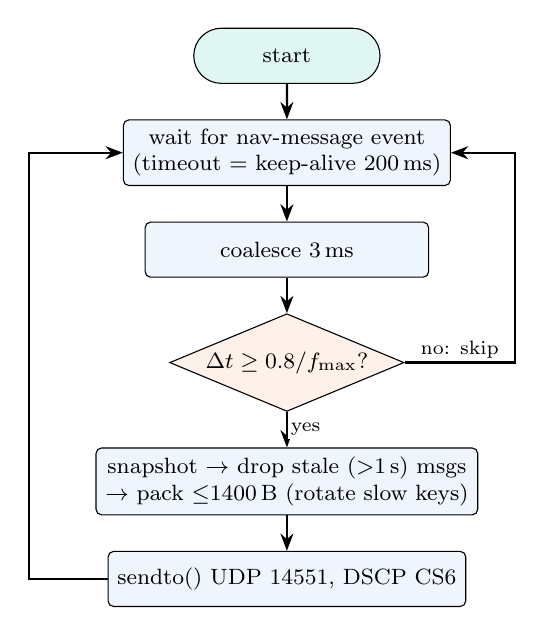
\begin{tikzpicture}[node distance=4.5mm]
  \node[term] (s) {start};
  \node[proc, below=of s] (w) {wait for nav-message event\\(timeout = keep-alive \SI{200}{\milli\second})};
  \node[proc, below=of w] (c) {coalesce \SI{3}{\milli\second}};
  \node[dec, below=of c] (g) {$\Delta t \ge 0.8/f_{\max}$?};
  \node[proc, below=of g] (p) {snapshot $\rightarrow$ drop stale ($>$\SI{1}{\second}) msgs\\$\rightarrow$ pack $\le$\SI{1400}{B} (rotate slow keys)};
  \node[proc, below=of p] (tx) {\code{sendto()} UDP 14551, DSCP CS6};
  \draw[arr] (s) -- (w);
  \draw[arr] (w) -- (c);
  \draw[arr] (c) -- (g);
  \draw[arr] (g) -- node[lbl,right]{yes} (p);
  \draw[arr] (p) -- (tx);
  \draw[arr] (g.east) -- node[lbl,above]{no: skip} ++(14mm,0) |- (w.east);
  \draw[arr] (tx.west) -- ++(-10mm,0) |- (w.west);
\end{tikzpicture}
\caption{Event-driven telemetry loop on the companion (\code{telemetry_streamer.py}).}
\label{fig:flow-telemetry}
\end{figure}

\paragraph{Wi-Fi QoS and power management} Telemetry, LiDAR and command packets carry
DSCP CS6 and video carries AF41. Under the RFC~8325 mapping \cite{rfc8325} these
are placed in the 802.11e/WMM voice and video access categories \cite{ieee80211e}, so
control traffic is not queued behind bulk video. Wi-Fi power saving is disabled on both
ends: when it is enabled, the station radio sleeps between beacons and buffers
incoming frames (commands, TCP ACKs) for \SIrange{10}{200}{\milli\second}.

\paragraph{Video without queueing} The camera thread drains the V4L2 queue
continuously with a driver buffer of one frame. The socket disables Nagle's algorithm
\cite{rfc896} and limits unsent data with \code{TCP_NOTSENT_LOWAT}. If the link is
still busy when a new frame is ready, that frame is \emph{dropped} rather than queued.
For control, a fresh frame is worth more than a complete sequence.
\code{--camera-passthrough} forwards the camera's own MJPEG bytes so the Pi does not
decode and re-encode.

\paragraph{Clock synchronisation and latency metrics} Every message carries the
sender's wall-clock capture time $t_s$. The receiver computes the raw one-way latency
and an \emph{excess} latency over a sliding \SI{10}{\second} window $W$:
\begin{equation}
  \ell_\text{raw}(k) = t_r(k) - t_s(k) - \delta_0, \qquad
  \ell_\text{excess}(k) = \ell_\text{raw}(k) - \min_{j\in W}\ell_\text{raw}(j).
  \label{eq:latency}
\end{equation}
$\ell_\text{raw}$ is absolute only when the clocks agree. \code{start_streams.py}
therefore makes the laptop the Pi's preferred \code{chrony} \cite{mills1991ntp}
source and steps the clock at start-up. $\ell_\text{excess}$ cancels any constant
offset and the fixed path delay, leaving queueing and Wi-Fi jitter. It is valid even
without synchronisation, and the health thresholds are applied to it
(warn \SI{150}{\milli\second}, error \SI{400}{\milli\second}). LiDAR scans are stamped
at the \emph{middle} of the revolution, $t_s=\tfrac12(t_\text{start}+t_\text{end})$,
because the samples are spread over the whole turn.

\paragraph{Revolution segmentation} The G2 firmware (v3.5) sets its "start of scan"
flag only every 3--4 revolutions. We saw only 2 flags per second at 6.4 rev/s. Relying on it merged several turns into one \SI{2}{\hertz} scan about
\SI{200}{\milli\second} old. The streamer instead detects a new revolution when the
packet start angle wraps, $\theta_\text{start} + 180^\circ < \theta_\text{start,prev}$.

\subsection{Odometry reconstruction without GNSS}
\label{sec:design-odom}

\paragraph{Source selection} \code{mavlink_to_ros2_bridge} publishes
\topic{/odom} and the \code{odom}$\rightarrow$\code{base_link} transform. If the
autopilot's EKF publishes \code{LOCAL_POSITION_NED}, that fused estimate is used
directly. Otherwise horizontal position is dead-reckoned from optical flow. Any
navigation message older than \SI{1}{\second} is treated as absent, so a sensor that
stops cannot freeze a stale position into the map.

\paragraph{Frame conversion} With NED position $(n,e,d)$ and ArduPilot Euler angles
$(\phi,\theta,\psi)$, $\psi$ clockwise from north, the ROS quantities are
\begin{equation}
  (x,y,z)_\text{ENU} = (e,\,n,\,-d), \qquad
  (\phi,\theta,\psi)_\text{ROS} = \left(\phi,\,-\theta,\,\operatorname{wrap}\!\left(\tfrac{\pi}{2}-\psi\right)\right).
  \label{eq:ned-enu}
\end{equation}

\paragraph{Optical-flow velocity} The MAVLink specification defines
\code{OPTICAL_FLOW.flow_comp_m_x/y} as metric velocity. ArduPilot instead fills them with
gyro-compensated angular flow rates $\omega_x,\omega_y$ (\si{\radian\per\second}),
each a rotation \emph{about} that axis. Following ArduPilot's EKF3 flow model, the
body-frame (FRD) velocity at height $h$ is
\begin{equation}
  v_{x}^{\text{FRD}} = -\,\omega_y\,h, \qquad v_{y}^{\text{FRD}} = \omega_x\,h,
  \label{eq:flow-ap}
\end{equation}
with $h$ taken from the flow message's ground distance, or from the rangefinder when
that is zero (as it is indoors without an EKF origin). For the integrated
\code{OPTICAL_FLOW_RAD} message, the gyro-integrated body rotation is subtracted
first: $v_x = (\Theta_y - \Gamma_y)h/\Delta t$ and
$v_y = -(\Theta_x - \Gamma_x)h/\Delta t$. Samples with quality below 20/255 are
discarded. The FRD$\rightarrow$FLU change negates $v_y$, and the body velocity is
rotated into the world frame by the ROS yaw $\psi_r$ and integrated:
\begin{equation}
  \begin{bmatrix} x \\ y \end{bmatrix}_{k+1} =
  \begin{bmatrix} x \\ y \end{bmatrix}_{k} +
  \begin{bmatrix} \cos\psi_r & -\sin\psi_r \\ \sin\psi_r & \cos\psi_r \end{bmatrix}
  \begin{bmatrix} v_x \\ -v_y \end{bmatrix}^{\!\text{FRD}} \Delta t_k ,
  \qquad 0 < \Delta t_k < \SI{1}{\second}.
  \label{eq:flow-integrate}
\end{equation}

\paragraph{Zero-velocity update (ZUPT)} Integrating noisy flow at rest produces drift. Following the
zero-velocity-detection literature \cite{foxlin2005pedestrian,skog2010zupt}, the
bridge declares the vehicle stationary when, over a window $W$ of
\SI{1}{\second} containing at least five samples spanning at least \SI{0.6}{\second},
\begin{equation}
  \sigma_W\!\left(\lVert\mathbf{f}\rVert\right) < \SI{15}{\milli\gacc}
  \quad\text{and}\quad
  \overline{\lVert\bm{\omega}\rVert}_W < \SI{4}{\degree\per\second},
  \label{eq:zupt}
\end{equation}
where $\mathbf{f}$ is specific force and $\bm{\omega}$ angular rate. While stationary,
or when telemetry is older than \SI{0.5}{\second} (a Wi-Fi drop-out), the integrated
velocity is forced to zero and position holds. The thresholds were chosen from a bench
log ($\sigma\approx\SI{3}{\milli\gacc}$, $\approx\SI{1}{\degree\per\second}$) and are
far below hover vibration levels. \Cref{sec:val-zupt} evaluates them.

\paragraph{Height source} With the bridge parameter \code{z_source} set to \code{auto}, height is taken from the first
available of: dedicated rangefinder, the flow module's ground distance (only when its
quality is sufficient), EKF local $-d$, and barometric altitude relative to the first
reading after start-up. Barometric altitude uses the standard-atmosphere relation
\cite{icao1993atmosphere}
\begin{equation}
  h_\text{baro} = 44\,330\left[1-\left(\frac{p}{1013.25\,\text{hPa}}\right)^{0.190295}\right]\ \text{m}.
  \label{eq:baro}
\end{equation}

\subsection{Planning and control}

\paragraph{Costmaps} Both costmaps are rolling windows in \code{odom}, so no prior map
or global localisation is needed. The local map is $8\times8$\,m at
\SI{5}{\hertz} and the global map $20\times20$\,m at \SI{1}{\hertz}, both at
\SI{0.05}{\metre} resolution. Obstacle marking and ray-tracing use \topic{/scan} over
\SIrange{0.10}{8.0}{\metre}. The \SI{8}{\metre} cap reflects the G2's reduced
reliability beyond that range indoors. The footprint radius is \SI{0.25}{\metre},
and cost decays outside it as Nav2's exponential inflation
\begin{equation}
  c(d) = 252\, e^{-\kappa\,(d - r_\text{robot})}, \qquad
  r_\text{robot} < d \le r_\text{infl},
  \label{eq:inflation}
\end{equation}
with $\kappa=3.0$ and $r_\text{infl}=\SI{0.40}{\metre}$.

\paragraph{Controller} The DWB local planner \cite{fox1997dwa} at \SI{10}{\hertz} is
configured as a \emph{holonomic} vehicle. Lateral velocity is sampled (15$\times$15
samples) over $\pm\SI{0.5}{\metre\per\second}$ with
\SI{0.5}{\metre\per\second\squared} acceleration limits, and yaw rate is fixed at zero:
a multirotor can translate in any direction without turning. Critics are
\code{Oscillation}, \code{BaseObstacle}, \code{PathAlign}, \code{PathDist} and
\code{GoalDist}. Yaw goal tolerance is effectively disabled
(\SI{3.15}{\radian}) and the $xy$ tolerance is \SI{0.20}{\metre}.

\paragraph{Behaviour tree for a flying base} Nav2's default recoveries (spin, back up)
are useless or harmful here: in simulation, backing up flew into the \SI{270}{\degree}
LiDAR's blind sector and hit a wall. The custom tree \code{navigate_drone.xml} replaces them with
costmap clearing followed by a \SI{3}{\second} hover, retried up to six times
\cite{colledanchise2018bt}.

\paragraph{Velocity command transformation} Nav2 emits body-frame (FLU) velocity
$(v_x,v_y,v_z,\dot\psi)$. The companion converts it to the
\code{SET_POSITION_TARGET_LOCAL_NED} setpoint using the latest autopilot heading
$\psi$ (clockwise from north):
\begin{equation}
  \begin{aligned}
  v_N &= \cos\psi\,v_x + \sin\psi\,v_y, &\quad v_E &= \sin\psi\,v_x - \cos\psi\,v_y,\\
  v_D &= -v_z, & \dot\psi_\text{NED} &= -\dot\psi ,
  \end{aligned}
  \label{eq:cmd}
\end{equation}
with \code{type_mask} $=1479$ (\texttt{0b010111000111}), so position, acceleration and
absolute yaw are ignored and velocity and yaw rate are used. If no heading has been
received, no setpoint is sent; the code does not guess.

\subsection{Layered safety design}
\label{sec:design-safety}

Safety is enforced at several independent layers (\cref{fig:safety}), so no single
software fault can command unsafe motion:
\begin{enumerate}[leftmargin=*,itemsep=1pt]
  \item \textbf{Human authority.} Arming and take-off are performed by the pilot on
    the RC transmitter. The laptop never auto-arms (\code{auto_arm=false}), and the
    listener forwards velocity \emph{only} while the vehicle is armed and in
    \code{GUIDED}. Switching the RC mode switch out of \code{GUIDED} returns control to
    the pilot immediately.
  \item \textbf{Speed envelope.} The ground bridge clamps horizontal speed to
    $\lVert(v_x,v_y)\rVert\le\SI{0.5}{\metre\per\second}$ by scaling the vector,
    which preserves its direction. The DWB limits are the same.
  \item \textbf{Liveness.} The ground bridge sends a stop when \topic{/cmd_vel} is older
    than \SI{0.5}{\second}. The Pi discards commands older than \SI{1}{\second}. The
    bridge publishes \code{/odom} at a \SI{10}{\hertz} fallback rate during drop-outs,
    so TF stays valid while position holds.
  \item \textbf{Vibration guard} (\code{vibration_motor_halt.py}, bench/optional). When
    vibration exceeds \SI{35}{\metre\per\second\squared}, it overrides the RC channels
    to \SI{40}{\percent} throttle (PWM \SI{1400}{\micro\second}) with level
    attitude, ignores stick input, and offers emergency disarm.
  \item \textbf{Autopilot failsafes.} RC-loss and low-battery actions configured in
    ArduPilot operate regardless of the companion.
\end{enumerate}

\begin{figure}[t]
\centering
\begin{tikzpicture}[node distance=4mm]
  \node[term] (in) {\topic{/cmd_vel} from Nav2};
  \node[proc, below=of in] (clamp) {ground: clamp $\lVert v_{xy}\rVert \le \SI{0.5}{\metre\per\second}$};
  \node[dec, below=of clamp] (fresh) {age $< \SI{0.5}{\second}$?};
  \node[proc, right=14mm of fresh] (stop) {send zero velocity};
  \node[proc, below=of fresh] (udp) {UDP 14553 $\rightarrow$ Pi listener};
  \node[dec, below=of udp] (armed) {armed $\wedge$ \code{GUIDED}?};
  \node[proc, right=14mm of armed] (drop) {do not forward\\(pilot in control)};
  \node[dec, below=of armed] (age) {cmd age $<\SI{1}{\second}$\\$\wedge$ heading known?};
  \node[proc, below=of age] (conv) {FLU$\rightarrow$NED (\cref{eq:cmd})};
  \node[term, below=of conv] (out) {\code{SET_POSITION_TARGET_LOCAL_NED}};
  \draw[arr] (in) -- (clamp);
  \draw[arr] (clamp) -- (fresh);
  \draw[arr] (fresh) -- node[lbl,right]{yes} (udp);
  \draw[arr] (fresh) -- node[lbl,above]{no} (stop);
  \draw[arr] (stop) |- (udp);
  \draw[arr] (udp) -- (armed);
  \draw[arr] (armed) -- node[lbl,right]{yes} (age);
  \draw[arr] (armed) -- node[lbl,above]{no} (drop);
  \draw[arr] (age) -- node[lbl,right]{yes} (conv);
  \draw[arr] (age.east) -| node[lbl,pos=0.25,above]{no} (drop.south);
  \draw[arr] (conv) -- (out);
\end{tikzpicture}
\caption{Command-path safety gating from Nav2 to the autopilot. The Pi re-evaluates
the gate on every new command and at a \SI{20}{\hertz} keep-alive.}
\label{fig:safety}
\end{figure}

\paragraph{Simulation-only LiDAR safety filter} In the PX4 simulation bridge, each
LiDAR return $i$ within reach $r_i\le r_\text{reach}=\SI{0.65}{\metre}$, with unit
bearing $\hat{\mathbf{u}}_i$, removes the commanded velocity component towards it:
\begin{equation}
  \mathbf{v} \leftarrow \mathbf{v} - \max\!\left(0,\ \mathbf{v}\cdot\hat{\mathbf{u}}_i\right)\hat{\mathbf{u}}_i ,
\end{equation}
applied in two passes. Returns closer than $r_\text{hard}=\SI{0.45}{\metre}$ add a
repulsion $-\sum_i (1-r_i/r_\text{hard})\,\hat{\mathbf{u}}_i$, scaled to at most
\SI{0.15}{\metre\per\second}. Unlike an earlier stop-all version, which froze the drone beside door frames, the
projection lets it slide along walls and back out of doorways. The same bridge yaws the vehicle towards
its direction of travel, because the simulated LiDAR is blind over the rear
\SI{90}{\degree}. Speed is scaled by $\max(0.25,\cos e_\psi)$ while turning, and by
0.1 when the heading error exceeds \SI{90}{\degree}.

\subsection{Hybrid semantic perception}
\label{sec:design-perception}

YOLOv8 instance segmentation \cite{redmon2016yolo,jocher2023yolov8} provides classes,
confidences and boxes in a few milliseconds. Its masks, however, are decoded from a
low-resolution prototype grid and are coarse at object boundaries. Segment Anything
\cite{kirillov2023sam,ravi2024sam2} produces sharp, class-agnostic masks when prompted.
The hybrid segmenter prompts SAM~2.1 with YOLO's boxes, so one image encoding is shared
by all instances. It then accepts each SAM mask only if four gates pass
(\cref{fig:seg-flow}). Otherwise it keeps the YOLO mask:
\begin{enumerate}[leftmargin=*,itemsep=1pt]
  \item SAM's predicted-IoU score $\ge 0.5$;
  \item the mask is clipped to the YOLO box grown by a 10\% margin (prevents leakage);
  \item the mask fills $\ge 5\%$ of the box (rejects slivers);
  \item $\text{IoU}(M_\text{SAM}, M_\text{YOLO}) \ge 0.3$ when a YOLO mask exists, which
    rejects SAM selecting a different object or a sub-part (e.g.\ a shirt instead of
    the person), where $\text{IoU}(A,B)=|A\cap B|/|A\cup B|$.
\end{enumerate}
Label images are rasterised from the largest mask to the smallest, so small objects on
top of large ones survive, and ties go to the more confident detection. YOLO runs in
FP16 on CUDA. SAM~1-family models are kept in FP32, because we got
empty masks from them in half precision. The default in the full stack is SAM at \SI{768}{px}: we
measured \SI{36}{\milli\second} inference and \SI{46}{\milli\second}
capture-to-result on the drone feed, against \SI{50}{\milli\second}/\SI{60}{\milli\second}
at \SI{1024}{px}, with near-identical masks.

\begin{figure}[H]
\centering
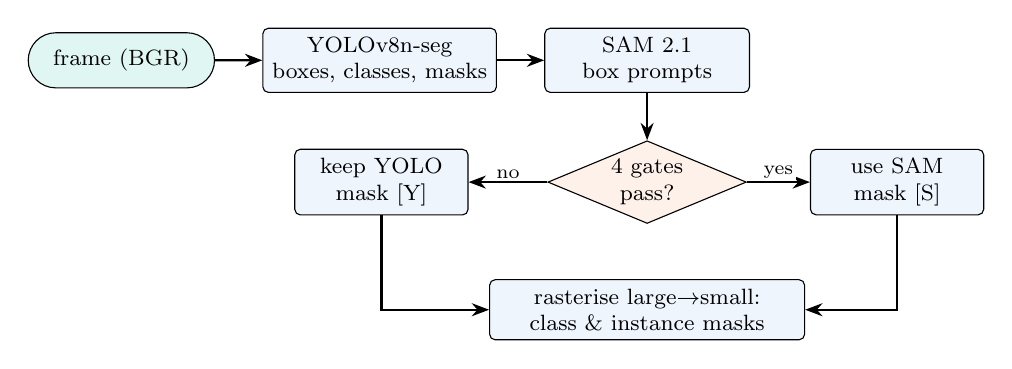
\begin{tikzpicture}[node distance=4mm and 6mm]
  \node[term] (f) {frame (BGR)};
  \node[proc, right=of f, minimum width=26mm] (y) {YOLOv8n-seg\\boxes, classes, masks};
  \node[proc, right=of y, minimum width=26mm] (s) {SAM 2.1\\box prompts};
  \node[dec, below=6mm of s] (g) {4 gates\\pass?};
  \node[proc, left=10mm of g, minimum width=22mm] (ky) {keep YOLO\\mask \code{[Y]}};
  \node[proc, right=8mm of g, minimum width=22mm] (ks) {use SAM\\mask \code{[S]}};
  \node[proc, below=7mm of g, minimum width=40mm] (r) {rasterise large$\rightarrow$small:\\class \& instance masks};
  \draw[arr] (f) -- (y);
  \draw[arr] (y) -- (s);
  \draw[arr] (s) -- (g);
  \draw[arr] (g) -- node[lbl,above]{no} (ky);
  \draw[arr] (g) -- node[lbl,above]{yes} (ks);
  \draw[arr] (ky) |- (r);
  \draw[arr] (ks) |- (r);
\end{tikzpicture}
\caption{Hybrid segmentation pipeline (\code{hybrid_segmenter.py}).}
\label{fig:seg-flow}
\end{figure}

\subsection{3D mapping from a 2D LiDAR}

\code{scan_to_3d} turns each horizontal scan into 3D points using the full
time-matched transform $\,^{o}\mathbf{T}_{l}(t)= {}^{o}\mathbf{T}_{b}(t)\,{}^{b}\mathbf{T}_{l}$
(height, roll, pitch, yaw and mount), so slices taken at different heights stack
into a volumetric map. Points fall into a \SI{5}{\centi\metre} voxel grid. A voxel is
published after two hits, and scans are skipped while tilt exceeds
\SI{30}{\degree}. The map is published at \SI{1}{\hertz} and saved as PLY. Its fidelity
is bounded by the height estimate and by horizontal flow drift.

\subsection{Observability: health metrics}

\code{metrics_monitor} republishes scalar health signals under \topic{/metrics/*}
(rates, jitter, latency, decode time, bandwidth, nearest obstacle, TF age, plan length,
command speed, CPU) and aggregates OK/WARN/FAIL into \topic{/diagnostics} and an RViz
overlay. One metric checks the whole TF and timing chain end to end. The
\emph{scan agreement} $\alpha$ is the fraction of LiDAR returns inside the local
costmap whose cell, or a direct neighbour, is lethal (value 100 in the published
\code{OccupancyGrid}):
\begin{equation}
  \alpha = \frac{\left|\{\,i : \max_{c\in\mathcal{N}_8(\text{cell}(\mathbf{p}_i))\cup\{\text{cell}(\mathbf{p}_i)\}} C(c) = 100\,\}\right|}{\left|\{\,i : \mathbf{p}_i \in \text{costmap}\}\right|}.
  \label{eq:agreement}
\end{equation}
Values of $\alpha\approx1$ show that the costmap reproduces what the LiDAR sees. A
drop reveals a wrong mount transform, stale TF or dropped scans.

%% ---------------------------------------------------------------------
\section{Design files summary}
\label{sec:designfiles}

All design files are in our repository. The system is defined almost
entirely by software and configuration. There are no custom PCBs and no
custom-fabricated parts: the sensors are fixed to the F450 frame with standard mounting
hardware (\cref{fig:hwphoto}), so no CAD files are required.
\Cref{tab:designfiles} lists the principal files. Third-party packages
(\code{m-explore-ros2}, \code{px4_msgs}) keep their upstream licences.

\begin{longtable}{p{5.6cm} p{2.0cm} p{2.1cm} p{4.6cm}}
\caption{Design files summary. Paths are relative to the repository root.
Licence: not yet chosen by the authors (see Specifications table).}
\label{tab:designfiles}\\
\toprule
\textbf{Design file} & \textbf{Type} & \textbf{Runs on} & \textbf{Purpose} \\
\midrule
\endfirsthead
\toprule
\textbf{Design file} & \textbf{Type} & \textbf{Runs on} & \textbf{Purpose} \\
\midrule
\endhead
\bottomrule
\endfoot
\code{raspberry_pi/start_streams.py} & Python & Pi & Supervisor: telemetry, LiDAR, camera, command streams; Wi-Fi power save; clock sync \\
\code{raspberry_pi/pixhawk_controller.py} & Python & Pi & MAVLink library: discovery, reconnection, arm/mode, telemetry extraction, flow conversion \\
\code{raspberry_pi/telemetry_streamer.py} & Python & Pi & Event-driven JSON telemetry, raw MAVLink, arm/mode command listener \\
\code{raspberry_pi/lidar_udp_streamer.py} & Python & Pi & YDLIDAR G2 protocol parser and binary UDP streamer \\
\code{raspberry_pi/camera_streamer.py} & Python & Pi & Low-latency MJPEG/JPEG TCP camera streamer \\
\code{raspberry_pi/mavlink_cmd_listener.py} & Python & Pi & Gated velocity-setpoint forwarder (FLU$\rightarrow$NED) \\
\code{raspberry_pi/vibration_motor_halt.py} & Python & Pi/laptop & Vibration guard with RC override \\
\code{raspberry_pi/99-pixhawk.rules}, \code{98-camera.rules} & udev & Pi & Persistent \code{/dev/pixhawk}, \code{/dev/camera} \\
\code{raspberry_pi/setup_pi.sh} & Shell & Pi & One-time Pi provisioning \\
\code{raspberry_pi/fake_pi.py} & Python & laptop & Synthetic telemetry/LiDAR for testing without a vehicle \\
\code{ros2_ws/src/gps_denied_bridge/} & ROS~2 pkg & laptop & Bridges, metrics monitor, 3D mapper \\
\code{ros2_ws/src/x500_navigation/config/nav2_real.yaml} & YAML & laptop & Nav2 parameters for the real vehicle \\
\code{ros2_ws/src/x500_navigation/launch/navigation_real.launch.py} & Launch & laptop & One-command ground bring-up \\
\code{ros2_ws/src/x500_navigation/behavior_trees/navigate_drone.xml} & BT XML & laptop & Drone-safe recovery tree \\
\code{ros2_ws/src/x500_navigation/worlds/make_office_world.py} & Python & laptop & Generates \code{office.sdf} simulation world \\
\code{ros2_ws/src/quadcopter_perception/} & ROS~2 pkg & laptop & Hybrid YOLO--SAM segmentation, tests \\
\code{ros2_ws/src/x500_px4_bridge/} & ROS~2 pkg & laptop & Simulation PX4 bridge, safety filter, Gazebo bridge \\
\code{scripts/setup_laptop_timeserver.sh} & Shell & laptop & \code{chrony} server set-up \\
\code{scripts/analysis.py} & Python & any & Regenerates trade-study charts \\
\code{report/scripts/*.py} & Python & laptop & Regenerate the validation figures and benchmark of this paper \\
\code{docs/*.md} & Markdown & -- & Problem statement, objectives, solutions, setup, quick start, reference \\
\end{longtable}

%% ---------------------------------------------------------------------
\section{Bill of materials}
\label{sec:bom}

\subsection{Design target (onboard configuration)}

\Cref{tab:bom-target} gives our costed bill of materials for the fully onboard
design target. Prices are in Indian rupees at the time of sourcing; links are in \code{docs/BOM.md}. The table covers the
avionics and sensing payload only; the airframe and propulsion can be reused from the
prototype (\cref{tab:bom-prototype}).

\begin{table}[H]
\centering\small
\caption{Design-target bill of materials (\code{docs/BOM.md}).}
\label{tab:bom-target}
\begin{tabularx}{\textwidth}{r p{4.2cm} L r r}
\toprule
\# & \textbf{Component} & \textbf{Function} & \textbf{Qty} & \textbf{Cost (INR)} \\
\midrule
1 & SC132GS stereo camera & Visual odometry, depth for avoidance, point clouds, ArUco & 1 & 6{,}061.66 \\
2 & Raspberry Pi~5, 8\,GB & Stereo depth, costmaps, avoidance, VO & 1 & 17{,}500.00 \\
3 & Holybro Kakute H7 V1.3 & Flight controller (STM32H7) running PX4 & 1 & 10{,}217.00 \\
4 & RadioMaster Pocket ELRS & Pilot transmitter, low-latency manual override & 1 & 7{,}000.00 \\
5 & RadioMaster RP1 ELRS Nano & Onboard RC receiver & 1 & 2{,}600.00 \\
6 & Tattu R-Line 850\,mAh 4S 150C & Flight battery ($\approx$\SI{10}{\minute} as recorded) & 1 & 2{,}300.00 \\
\midrule
\multicolumn{4}{r}{\textbf{Total}} & \textbf{45{,}678.66} \\
\bottomrule
\end{tabularx}
\end{table}

\noindent\emph{Note.} The battery we listed
($\approx$\SI{10}{\minute} flight) does not meet the $\ge$\SI{30}{\minute}
endurance objective. Meeting that objective will need a larger battery and a
re-evaluated payload budget (\cref{sec:limitations}).

\subsection{Current prototype}

\Cref{tab:bom-prototype} lists the components of the prototype we built and where each
came from. \Cref{tab:bom-spend} lists everything we bought for it under the Design
Practicum course, with prices including GST as invoiced. The total spend was
\INR{52{,}714}. The Pixhawk~6C, YDLIDAR~G2, USB camera, flight battery and RC
transmitter came from laboratory stock and were not purchased.

\begin{table}[H]
\centering\small
\caption{Components of the implemented prototype.}
\label{tab:bom-prototype}
\begin{tabularx}{\textwidth}{p{3.3cm} L p{2.9cm}}
\toprule
\textbf{Component} & \textbf{Specification as used} & \textbf{Source} \\
\midrule
Flight controller & Holybro Pixhawk~6C, ArduPilot ArduCopter, USB MAVLink 115\,200 baud, anti-vibration mount & lab stock; mount \#3 \\
Companion computer & Raspberry Pi~5 (4\,GB), 64\,GB microSD, aarch64 Linux, Python~3 & \#5, \#13 \\
2D LiDAR & YDLIDAR G2, USB--serial 115\,200 baud, 360 bins & lab stock \\
Optical flow + range & MTF-01 flow/range module on the autopilot & \#9 \\
Camera & USB~2.0 UVC (Arkmicro \code{18ec:3399}), 640$\times$480 MJPEG & lab stock \\
RC system & RadioMaster RP1 V2 ExpressLRS receiver on the autopilot & \#2; transmitter lab stock \\
Airframe & F450 quadrotor kit (\SI{450}{\milli\metre}) with propeller guards & \#4, \#8 \\
Propulsion & 4$\times$ A2212 \SI{1000}{KV} motors, 4$\times$ \SI{30}{\ampere} SimonK ESCs, 1045 propellers & \#16, \#10/\#12, \#14 \\
Power & 3S \SI{2200}{\milli\ampere\hour} LiPo; \SI{5.3}{\volt}/\SI{3}{\ampere} power module & battery lab stock; \#7 \\
Ground computer & Laptop, Ubuntu 22.04, NVIDIA RTX~4050 Laptop GPU & own \\
\bottomrule
\end{tabularx}
\end{table}

\begin{table}[H]
\centering\small
\caption{Purchases for the prototype (Design Practicum, Group~66; prices in INR
including GST, from the supplier invoices).}
\label{tab:bom-spend}
\begin{tabularx}{\textwidth}{r L r r l}
\toprule
\# & \textbf{Item} & \textbf{Qty} & \textbf{Cost (INR)} & \textbf{Use} \\
\midrule
1 & Pixhawk 2.4.8 flight controller & 1 & 8{,}201.00 & not used (Pixhawk~6C flown) \\
2 & RadioMaster RP1 V2 ExpressLRS nano receiver & 1 & 3{,}032.60 & fitted \\
3 & Anti-vibration mount for Pixhawk & 1 & 185.26 & fitted \\
4 & F450 quadcopter frame kit & 1 & 895.62 & fitted \\
5 & Raspberry Pi~5, 4\,GB & 1 & 15{,}540.60 & fitted \\
6 & IMX219 camera module & 1 & 7{,}375.00 & not used (USB camera used) \\
7 & \SI{5.3}{\volt} \SI{3}{\ampere} power module & 1 & 619.50 & fitted \\
8 & F450 propeller guard set & 1 & 436.60 & fitted \\
9 & MTF-01 optical-flow and ranging module & 1 & 5{,}864.60 & fitted \\
10 & SimonK \SI{30}{\ampere} ESC, pack of 4 & 1 & 1{,}950.00 & fitted / spare \\
11 & \SI{1800}{KV} brushless motor & 4 & 2{,}396.00 & not used \\
12 & SimonK \SI{30}{\ampere} ESC & 5 & 1{,}595.00 & fitted / spare \\
13 & SanDisk Ultra 64\,GB microSD card & 1 & 1{,}899.00 & fitted \\
14 & 1045 propellers (CW + CCW pair) & 4 & 380.00 & fitted \\
15 & CP2102 USB--UART adapter & 2 & 258.00 & set-up and debugging \\
16 & A2212 \SI{1000}{KV} brushless motor & 5 & 2{,}075.00 & 4 fitted, 1 spare \\
-- & Marketplace fees and invoice rounding & -- & 10.22 & -- \\
\midrule
\multicolumn{3}{r}{\textbf{Total}} & \textbf{52{,}714.00} & \\
\bottomrule
\end{tabularx}
\end{table}

\noindent Of the total, \INR{17{,}972} went on items that did not end up on the vehicle
(\#1, \#6, \#11).

\subsection{Software bill of materials}

\begin{table}[H]
\centering\small
\caption{Principal software dependencies.}
\label{tab:sbom}
\begin{tabularx}{\textwidth}{l l L}
\toprule
\textbf{Component} & \textbf{Version} & \textbf{Use} \\
\midrule
Ubuntu / ROS~2 & 22.04 / Humble & Ground middleware \\
Nav2, SLAM Toolbox & Humble releases & Planning, costmaps; SLAM in simulation \\
ArduPilot & ArduCopter (GUIDED mode) & Prototype autopilot \\
PX4 + Gazebo Harmonic & PX4 \code{main}, gz 8 & Simulation \\
pymavlink, pyserial & $\ge$2.4.40, $\ge$3.5 & Companion MAVLink and serial \\
OpenCV, NumPy & distribution packages & Camera, image transport \\
Ultralytics & 8.4.70 (benchmark host) & YOLOv8n-seg, SAM~2.1 inference \\
PyTorch / CUDA & 2.5.1 / 12.1 (benchmark host) & GPU inference \\
chrony, iw & distribution packages & Clock sync, Wi-Fi power management \\
\bottomrule
\end{tabularx}
\end{table}

%% ---------------------------------------------------------------------
\section{Build instructions}
\label{sec:build}

\noindent\fcolorbox{red!60!black}{red!5}{\parbox{\dimexpr\textwidth-2\fboxsep-2\fboxrule}{\small
\textbf{Safety.} Remove all propellers during assembly and bench testing. Never power
the motors with the companion computer connected for the first time. Check the RC
override and failsafes before every autonomous flight. Lithium-polymer batteries
must be charged and stored per the manufacturer's instructions.}}

\subsection{Mechanical integration}
\label{sec:build-mech}

\begin{enumerate}[leftmargin=*,itemsep=2pt]
  \item Mount the flight controller on vibration isolation at the airframe's centre
    of gravity, arrow forward, as for any ArduPilot build. Confirm normal manual
    flight \emph{before} adding the companion.
  \item Mount the Raspberry Pi where its USB ports are reachable and it receives
    airflow. A Pi under sustained load needs a heatsink.
  \item Mount the YDLIDAR G2 with an unobstructed horizontal field of view. Propeller
    arms and landing gear in the scan plane appear as permanent obstacles. Returns
    closer than \SI{0.10}{\metre} (costmap) and \SI{0.12}{\metre} (streamer) are
    rejected, but larger airframe parts must be kept out of the plane or masked.
    Record the mount offset (\cref{sec:build-calib}).
  \item Mount the downward optical-flow/range module with a clear view of the floor,
    away from propeller downwash and legs, oriented per ArduPilot's
    \code{FLOW_ORIENT_YAW} convention.
  \item Mount the camera facing forward and record its offset.
  \item Route the USB cables with strain relief. A connector that is pulled loose in
    flight removes that sensor; the supervisor restarts the stream when the device
    returns.
\end{enumerate}

\subsection{Electrical integration}

Follow \cref{fig:wiring}. Connect the autopilot to the Pi by USB (simplest and
recommended). Connect the LiDAR adapter and camera to the Pi's other USB ports. Supply
the Pi from a dedicated \SI{5}{\volt} regulator rated at least \SI{3}{\ampere}. The
flow/range module and RC receiver connect to the autopilot as documented by
ArduPilot.

\subsection{Companion computer provisioning}

On the Pi, which needs only the \code{raspberry_pi/} directory:
\begin{lstlisting}[language=bash]
# from the laptop: copy code (repeat after every change)
rsync -av --exclude '*.pt' --exclude '__pycache__' \
  ~/gps-denied-vtol/raspberry_pi/ <user>@<pi_ip>:~/raspberry_pi/

# on the Pi
cd ~/raspberry_pi
sudo apt install -y python3-opencv python3-numpy
pip install -r requirements.txt --break-system-packages
sudo ./setup_pi.sh            # udev rules, dialout, chrony, iw, sudoers entries
# log out and in once, then verify:
ls -la /dev/pixhawk /dev/camera /dev/ttyUSB0
python3 test_connection.py    # must end with [PASSED]
\end{lstlisting}
Other autopilot or camera models are supported by adding their USB vendor/product IDs
to \code{99-pixhawk.rules} or \code{98-camera.rules}.

\subsection{Ground computer provisioning}

Requirements: Ubuntu 22.04, ROS~2 Humble and an NVIDIA GPU.
\begin{lstlisting}[language=bash]
sudo apt install -y python3-colcon-common-extensions python3-rosdep
sudo rosdep init; rosdep update
git clone https://github.com/DEEPAKSINGLA-byte/gps-denied-vtol.git ~/gps-denied-vtol
cd ~/gps-denied-vtol/ros2_ws && source /opt/ros/humble/setup.bash
rosdep install --from-paths src --ignore-src -r -y
colcon build --symlink-install
pip install -U ultralytics                 # YOLO + SAM

# disable Wi-Fi power saving and serve time to the Pi
printf '[connection]\nwifi.powersave = 2\n' | \
  sudo tee /etc/NetworkManager/conf.d/wifi-powersave-off.conf
sudo systemctl restart NetworkManager
sudo ~/gps-denied-vtol/scripts/setup_laptop_timeserver.sh
\end{lstlisting}
Model weights (\code{yolov8n-seg.pt}, \code{sam2.1_t.pt}) are resolved from the
workspace root, so they are not re-downloaded at every launch. A laptop connected to
the drone's hotspot is usually offline, and the segmentation node would otherwise
fail. Connect Pi and laptop directly (e.g.\ a \SI{5}{\giga\hertz} laptop hotspot).
Relaying through a phone hotspot sends each packet over the air twice.

\subsection{Autopilot configuration}

\begin{table}[H]
\centering\small
\caption{ArduPilot parameters for indoor GPS-denied operation (\code{docs/SETUP.md}).}
\label{tab:apparams}
\begin{tabularx}{\textwidth}{l l L}
\toprule
\textbf{Parameter} & \textbf{Value} & \textbf{Reason} \\
\midrule
\code{FLTMODEx} & \code{GUIDED} (4) on one switch position & The laptop can steer only in GUIDED \\
\code{EK3_SRC1_POSXY} & 0 (none) or 4 (optical flow) & No GNSS indoors \\
\code{EK3_SRC1_POSZ} & 1 (baro) or 2 (rangefinder) & Height source \\
\code{AHRS_GPS_USE} & 0 & Do not use GPS \\
\code{ARMING_CHECK} & 1048558 & Skips GPS/compass checks that otherwise block arming (\code{PreArm: Need 3D Fix}) \\
RC-loss, battery failsafes & per vehicle & Must land/hold without GNSS \\
\bottomrule
\end{tabularx}
\end{table}

\subsection{Sensor extrinsic calibration}
\label{sec:build-calib}

The mount transforms in \code{navigation_real.launch.py} are placeholders:
LiDAR $(0,0,-0.15)$\,m and camera $(0.10,0,0.05)$\,m, both with zero rotation.
\begin{enumerate}[leftmargin=*,itemsep=1pt]
  \item Measure the translation from the flight controller's centre to the LiDAR's
    optical centre and to the camera, in FLU axes.
  \item Measure the LiDAR's yaw relative to the airframe's forward axis. The receiver
    also exposes \code{angle_offset_deg} and \code{clockwise_input}.
  \item Edit the static transform arguments, rebuild (\code{colcon build}), relaunch.
  \item Validate. With the vehicle carried slowly by hand past walls, the scan must
    stay registered to the costmap. \topic{/metrics/costmap/local/scan_agreement}
    should remain close to 1, and a value well below 1 indicates a wrong mount yaw or
    timing.
\end{enumerate}
Optical-flow sign errors are corrected on the autopilot (\code{FLOW_ORIENT_YAW}), or
for a pure $x$ flip with the bridge parameter \code{optical_flow_scale}$=-1$.

%% ---------------------------------------------------------------------
\section{Operation instructions}
\label{sec:operation}

\subsection{Start-up sequence}

The ground computer must be started first, because the camera stream is a TCP
connection initiated by the Pi towards a listening laptop.
\Cref{fig:opflow} summarises the procedure.

\begin{lstlisting}[language=bash]
# 1. Laptop
cd ~/gps-denied-vtol/ros2_ws && source install/setup.bash
ros2 launch x500_navigation navigation_real.launch.py pi_ip:=<pi_ip>
#    options: camera:=false segmentation:=false rviz:=false map3d:=false
#             seg_sam_imgsz:=768|1024  seg_sam_model:=none

# 2. Raspberry Pi
ssh <user>@<pi_ip>
cd ~/raspberry_pi && python3 start_streams.py --nav-cmds
#    look for: "clock synced to laptop ... offset ..."
\end{lstlisting}

\begin{figure}[H]
\centering
\begin{tikzpicture}[node distance=4mm]
  \node[term] (a) {Props off (first time)};
  \node[proc, below=of a] (b) {Laptop: \code{navigation_real.launch.py}};
  \node[proc, below=of b] (c) {Pi: \code{start_streams.py --nav-cmds}};
  \node[dec, below=of c] (d) {RViz status OK?\\rates nominal?};
  \node[proc, right=12mm of d, minimum width=30mm] (fix) {troubleshoot\\(\cref{tab:troubleshoot})};
  \node[proc, below=of d] (e) {hand-carry test: scan\\stays registered to map};
  \node[proc, below=of e] (f) {RC: arm, take off (\code{ALT_HOLD})};
  \node[proc, below=of f] (g) {RC: switch to \code{GUIDED}};
  \node[proc, below=of g] (h) {RViz: Nav2 Goal};
  \node[dec, below=of h] (i) {anomaly?};
  \node[proc, right=12mm of i, minimum width=30mm] (j) {RC: switch out\\of \code{GUIDED}};
  \node[term, below=of i] (k) {RC: land, disarm; Ctrl-C Pi, then laptop};
  \draw[arr] (a)--(b); \draw[arr] (b)--(c); \draw[arr] (c)--(d);
  \draw[arr] (d)--node[lbl,above]{no}(fix); \draw[arr] (fix.north) |- (c.east);
  \draw[arr] (d)--node[lbl,right]{yes}(e); \draw[arr] (e)--(f); \draw[arr] (f)--(g);
  \draw[arr] (g)--(h); \draw[arr] (h)--(i);
  \draw[arr] (i)--node[lbl,above]{yes}(j); \draw[arr] (j) |- (k.east);
  \draw[arr] (i)--node[lbl,right]{no / goal reached}(k);
\end{tikzpicture}
\caption{Operating procedure for a supervised autonomous flight.}
\label{fig:opflow}
\end{figure}

\subsection{Pre-flight checks}

\begin{itemize}[leftmargin=*,itemsep=1pt]
  \item RViz shows the scan, camera and both costmaps, and the diagnostics overlay
    reads OK.
  \item Nominal topic rates (documented in \code{docs/QUICKSTART.md}):
    \topic{/odom} $\approx$\SI{30}{\hertz}, \topic{/scan} $\approx$\SI{7}{\hertz},
    \topic{/camera/image_raw} $\approx$\SI{15}{\hertz} (camera-limited),
    \topic{/segmentation/detections} $\approx$\SI{15}{\hertz}. Check with
    \code{ros2 topic hz}.
  \item Carried by hand, the vehicle moves in RViz and the scan stays aligned with the
    costmap.
  \item The RC override has been tested: switching out of \code{GUIDED} stops
    autonomous motion.
\end{itemize}

\subsection{Flight}

\begin{enumerate}[leftmargin=*,itemsep=1pt]
  \item Arm and take off with the RC transmitter. \code{ALT_HOLD} is recommended
    first; \code{POSHOLD} requires optical flow.
  \item Switch to \code{GUIDED} with the RC mode switch. The laptop cannot arm the
    vehicle or change its mode for the pilot.
  \item In RViz, set a \emph{Nav2 Goal}. The vehicle follows only while armed and in
    \code{GUIDED}, at no more than \SI{0.5}{\metre\per\second}, and stops when
    commands cease for \SI{0.5}{\second}.
  \item To take over, switch out of \code{GUIDED}. Land and disarm with the RC, then
    stop the Pi, then the laptop.
\end{enumerate}
Fly in visual line of sight, in a clear area, with a spotter, and never over people.

\subsection{Monitoring and logging}

Every health signal is a ROS topic under \topic{/metrics/} and can be plotted in
PlotJuggler or \code{rqt_plot}. The 3D map is saved on shutdown to
\code{~/drone_maps/map3d_*.ply}, or on demand with the \code{/map_3d/save} service.
The Pi tool \code{sensor_telemetry.py --log flight.csv} records autopilot telemetry
directly; this is how the bench data in \cref{sec:val-bench} were obtained.

\subsection{ROS-free and bench tools}

With the propellers removed, \code{drone_cli.py}, \code{arm_disarm.py} and
\code{set_mode.py} arm, disarm and change mode. \code{arm_disarm.py --arm --force}
bypasses pre-arm checks for bench use. \code{live_segmentation.py} and
\code{camera_receiver.py} run perception or a viewer on the laptop without ROS.
\code{fake_pi.py} replays synthetic telemetry and LiDAR into the ground stack for
testing without hardware.

\subsection{Troubleshooting}

\begin{table}[H]
\centering\small
\caption{Common faults (\code{docs/QUICKSTART.md}, \code{raspberry_pi/README.md}).}
\label{tab:troubleshoot}
\begin{tabularx}{\textwidth}{p{4.3cm} L}
\toprule
\textbf{Symptom} & \textbf{Action} \\
\midrule
No \topic{/odom} & Is \code{start_streams.py} running, targeting the laptop IP? Open firewall: \code{ufw allow 14550:14553/udp}, \code{ufw allow 5000/tcp} \\
\code{Timed out waiting for heartbeat} & Autopilot powered and enumerated? \code{ls -la /dev/pixhawk}; \code{test_connection.py} \\
\code{Device or resource busy} & Another process owns the autopilot port (\code{lsof /dev/pixhawk}) \\
No \topic{/scan} & LiDAR on \code{/dev/ttyUSB0}? (the supervisor retries) \\
No camera & Start the laptop before the Pi; do not run stand-alone tools on the same port \\
Goals ignored & Pi started with \code{--nav-cmds}? Vehicle armed \emph{and} in \code{GUIDED}? \\
\code{Arming DENIED} & Read the reason; indoors apply \cref{tab:apparams} \\
High latency & Disable Wi-Fi power save; direct link; smaller frames (\code{--camera-size 424x240}) \\
Throttle locked at 40\% & Vibration guard tripped: release (\code{r}) or disarm (\code{d}), inspect propellers/motors \\
\bottomrule
\end{tabularx}
\end{table}

\subsection{Simulation}
\label{sec:op-sim}

The simulation uses PX4 SITL in Gazebo Harmonic, connected to ROS~2 by the
Micro~XRCE-DDS agent. It is not ArduPilot. The apt \code{ros_gz_bridge} for Humble
targets Gazebo Fortress and receives nothing from Harmonic, so we wrote a
bridge built on Harmonic's Python transport bindings.
\begin{itemize}[leftmargin=*,itemsep=1pt]
  \item \code{ros2 launch x500_navigation sim_baylands.launch.py}: x500 with a
    \SI{270}{\degree}, \SI{30}{\metre} 2D LiDAR in PX4's Baylands park, spawned in a tree
    grove. The vehicle arms and climbs to \SI{2}{\metre} automatically. SLAM~Toolbox
    maps and Nav2 plans; the bridge flies OFFBOARD at up to \SI{1}{\metre\per\second}.
  \item \code{ros2 launch x500_navigation sim_office.launch.py}: a generated
    $24\times16$\,m office (open-plan area, meeting room, kitchen, offices, server
    room, \SI{2.5}{\metre} corridor, \SI{1.6}{\metre} doorways). Flight is at
    \SI{1.5}{\metre} and \SI{0.5}{\metre\per\second}, with autonomous frontier
    exploration \cite{yamauchi1997frontier} (\code{explore_lite}) that returns to the
    lobby when no frontier remains.
\end{itemize}
The office was designed around the 2D LiDAR's blind spots. Furniture is either
$\le$\SI{1.1}{\metre} tall (flown over and not seen) or $\ge$\SI{2}{\metre} tall (seen
and avoided), with nothing in between. Flying below about \SI{1.3}{\metre} would allow
collisions with furniture the LiDAR cannot see. In simulation, PX4's estimator still
uses simulated GNSS: the LiDAR is used for mapping and avoidance, but is not fed back
into the autopilot's state estimate.

%% ---------------------------------------------------------------------
\section{Validation and characterisation}
\label{sec:validation}

\subsection{Scope and evidence levels}

\Cref{tab:evidence} shows where each result comes from. Items marked \emph{logged}
come with data in the repository, and their figures can be regenerated from
\code{report/scripts/}. Items marked \emph{dev.\ notes} are measurements we took during
development without keeping the raw data. We tested the real vehicle in a \SI{7}{\minute} hover over grass, measured against ground marks, and
in an autonomous square-path flight with obstacle avoidance (\cref{sec:val-hwdemo}).
Simulation flights, with Gazebo ground truth, are analysed in \cref{sec:val-simlogs}.

\begin{table}[H]
\centering\small
\caption{Validation evidence and its provenance.}
\label{tab:evidence}
\begin{tabularx}{\textwidth}{p{4.6cm} p{2.0cm} L}
\toprule
\textbf{Item} & \textbf{Source} & \textbf{Basis} \\
\midrule
Unit tests of segmentation logic & logged & 17 tests executed, \cref{sec:val-tests} \\
Bench sensor characterisation & logged & 25\,s autopilot log, \code{report/data/bench_telemetry_2026-11-15.csv} \\
ZUPT detector evaluation & logged & same log, bridge's parameters \\
IMU dead-reckoning drift & logged & same log, strapdown integration \\
Segmentation timing & logged & 100 frames $\times$ 3 configurations on RTX~4050 \\
Link-latency reductions & dev.\ notes & \code{docs/REFERENCE.md}, single-host measurement \\
Segmentation latency on drone feed & dev.\ notes & launch-file comment, \code{docs/REFERENCE.md} \\
Topic rates on the real vehicle & dev.\ notes & \code{docs/QUICKSTART.md} \\
LiDAR revolution rate, flag rate & dev.\ notes & source comment, \code{lidar_udp_streamer.py} \\
Real-vehicle hover drift & logged & \SI{7}{\minute} \code{GUIDED} hover at \SI{2.5}{\metre} over grass, ground marks \\
Autonomous square path + avoidance & logged & video (\cref{fig:hwdemo}) \\
Simulation behaviour & dev.\ notes & qualitative, \code{docs/SIMULATION.md}, video (\cref{fig:sim}) \\
Simulation flight metrics & logged & 26 PX4 SITL logs with Gazebo truth, \cref{sec:val-simlogs} \\
\bottomrule
\end{tabularx}
\end{table}

\subsection{Software unit tests}
\label{sec:val-tests}

The perception package contains 17 \code{pytest} cases for the ROS-independent fusion
and rasterisation logic. They check mask IoU, box expansion and clipping, acceptance of
a good SAM mask, fallback on a low SAM score, fallback on SAM--YOLO disagreement,
clipping of leaked masks, rejection of empty masks, selective refinement, the
detect-only model path, the no-SAM path, overlap ordering in rasterisation, and
SAM-family detection. All 17 passed on the benchmark host (\code{17 passed in
0.10s}). The ROS packages additionally carry the standard \code{flake8},
\code{pep257} and copyright tests.

\subsection{Bench characterisation of the autopilot sensors}
\label{sec:val-bench}

\paragraph{Protocol} The vehicle stood on a bench, disarmed, with no flight battery
connected (reported battery voltage \SI{0.19}{\volt}) and no GNSS fix
(0 satellites, fix type 0). Telemetry streamed from the Pi was logged on the laptop by
\code{plotjuggler_bridge.py} on 2026-11-15, for \SI{24.93}{\second} (243 samples).
The log predates the \SI{30}{\hertz} telemetry change, so the median rate was
\SI{9.91}{\hertz} (spacing $\SI{103.0}{}\pm\SI{17.0}{\milli\second}$, longest gap
\SI{302.6}{\milli\second}). The vehicle was pitched \SI{12.96}{\degree}, and the
disturbances near \SI{5}{\second} and \SIrange{13}{16}{\second} are unannotated.

\begin{figure}[t]
\centering
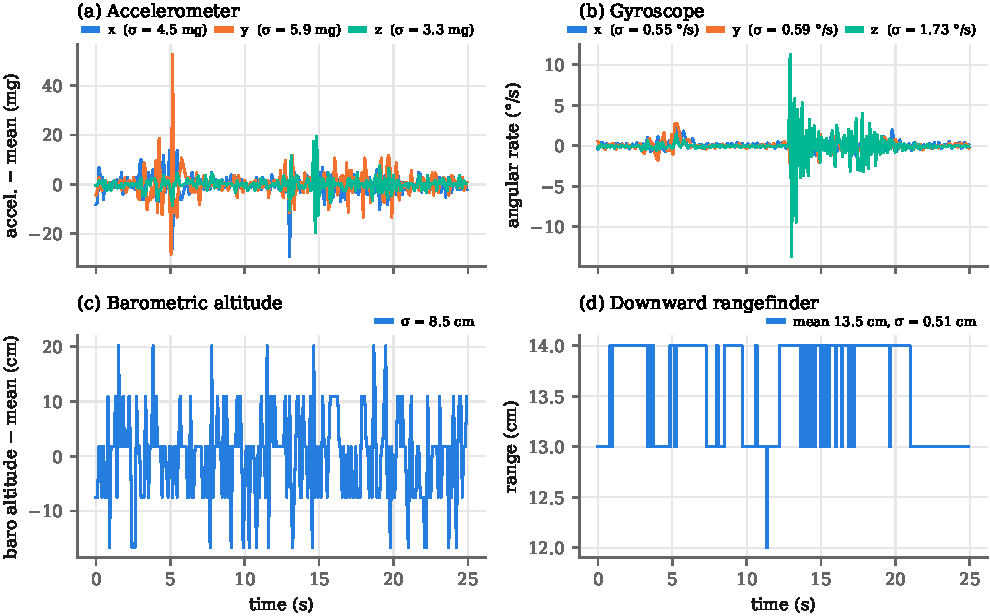
\includegraphics[width=\textwidth]{bench_sensor_noise.pdf}
\caption{Stationary bench log, vehicle disarmed. (a) Accelerometer deviation from the
mean; (b) gyroscope rate; (c) altitude computed from static pressure with
\cref{eq:baro}; (d) downward rangefinder. A transient disturbance is visible near
\SI{13}{\second}, mainly about the yaw axis.}
\label{fig:bench}
\end{figure}

\begin{table}[H]
\centering\small
\caption{Sensor statistics from the bench log (\cref{fig:bench}). $\sigma$ is the
standard deviation over the whole log, including the disturbances.}
\label{tab:bench}
\begin{tabular}{l S[table-format=4.1] S[table-format=1.2] l}
\toprule
\textbf{Channel} & {\textbf{Mean}} & {$\bm{\sigma}$} & \textbf{Remark} \\
\midrule
Accel $x$ (\si{\milli\gacc}) & 199.1 & 4.47 & pitch $\approx$\SI{13}{\degree} projects gravity \\
Accel $y$ (\si{\milli\gacc}) & 14.3 & 5.93 & \\
Accel $z$ (\si{\milli\gacc}) & -983.6 & 3.29 & $\lVert\mathbf{f}\rVert = 1003.6\pm\SI{2.9}{\milli\gacc}$ \\
Gyro $x$ (\si{\degree\per\second}) & 0.096 & 0.55 & \\
Gyro $y$ (\si{\degree\per\second}) & 0.030 & 0.59 & \\
Gyro $z$ (\si{\degree\per\second}) & -0.053 & 1.73 & inflated by the yaw transient \\
Static pressure (\si{\hecto\pascal}) & 895.01 & 0.0092 & resolution \SI{0.01}{\hecto\pascal} \\
Baro altitude (\si{\centi\metre}) & {--} & 8.46 & peak-to-peak \SI{36.8}{\centi\metre} \\
Rangefinder (\si{\centi\metre}) & 13.55 & 0.51 & \SI{1}{\centi\metre} quantisation \\
\bottomrule
\end{tabular}
\end{table}

\paragraph{Findings} $\sigma\lVert\mathbf{f}\rVert=\SI{2.9}{\milli\gacc}$ matches the
noise assumed for the ZUPT thresholds. Barometric altitude is noisy at decimetre level
($\sigma=\SI{8.5}{\centi\metre}$, \SI{37}{\centi\metre} peak-to-peak), mostly from the
\SI{0.01}{\hecto\pascal} ($\approx\SI{9}{\centi\metre}$) pressure quantisation, which
justifies ranking the rangefinder ahead of the barometer. The rangefinder, at
\SI{13.5}{\centi\metre} above the floor, toggled between adjacent centimetre codes
($\sigma=\SI{0.5}{\centi\metre}$).

\subsection{Zero-velocity detector}
\label{sec:val-zupt}

The bridge's detector (\cref{eq:zupt}) was re-implemented offline with identical
parameters and applied to the log (\cref{fig:zupt}). Of 237 complete \SI{1}{\second}
windows, \SI{96.2}{\percent} were classified stationary. The specific-force criterion
was never violated: maximum windowed $\sigma=\SI{10.4}{\milli\gacc}$ against a
\SI{15}{\milli\gacc} threshold, median \SI{1.6}{\milli\gacc}. The remaining
\SI{3.8}{\percent} were rejected by the angular-rate criterion, all during the event
at \SIrange{13}{15}{\second}, where the windowed mean $\lVert\bm\omega\rVert$ reached
\SI{6.45}{\degree\per\second} (median \SI{0.43}{\degree\per\second}). This was a real
rotation (heading changed about \SI{1}{\degree}), so withholding the update is correct.
Both statistics sit about an order of magnitude below their thresholds at rest.

\begin{figure}[H]
\centering
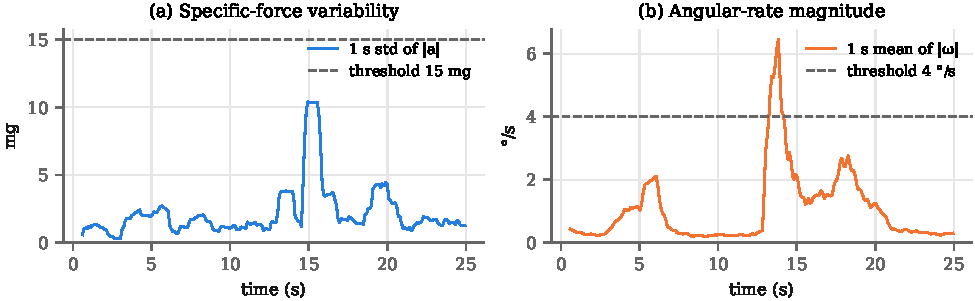
\includegraphics[width=\textwidth]{zupt_detector.pdf}
\caption{ZUPT detector statistics on the bench log with the bridge's thresholds
(dashed). Stationary requires both curves below their thresholds.}
\label{fig:zupt}
\end{figure}

\subsection{Inertial dead-reckoning drift}
\label{sec:val-dr}

The specific force was rotated into NED with the logged attitude, gravity removed,
and integrated twice, with the stationary vehicle as ground truth. The experiment is
intentionally simple (no filter, \SI{10}{\hertz}) and shows error growth, not the
autopilot EKF's performance.

\begin{figure}[H]
\centering
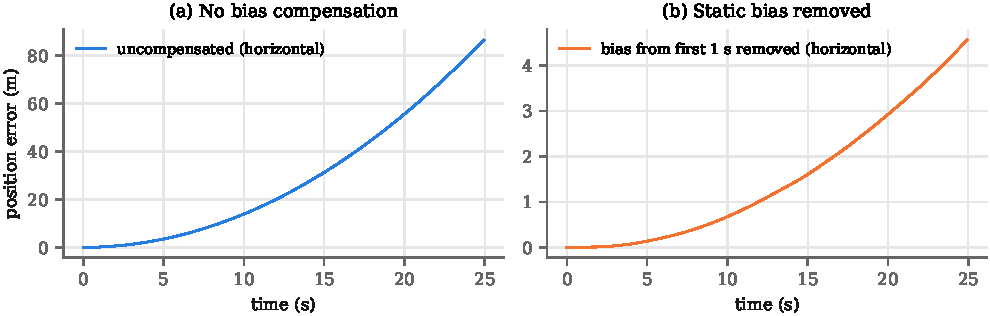
\includegraphics[width=\textwidth]{imu_dead_reckoning.pdf}
\caption{Horizontal position error of strapdown integration on the stationary log.
(a) Uncompensated; (b) after subtracting the mean NED acceleration of the first
second.}
\label{fig:dr}
\end{figure}

\begin{table}[H]
\centering\small
\caption{Horizontal dead-reckoning error on a stationary vehicle.}
\label{tab:dr}
\begin{tabular}{l S[table-format=2.2] S[table-format=2.2] S[table-format=2.2] S[table-format=2.2]}
\toprule
& {$t=\SI{5}{\second}$} & {$t=\SI{10}{\second}$} & {$t=\SI{20}{\second}$} & {$t=\SI{24.9}{\second}$} \\
\midrule
Uncompensated (\si{\metre}) & 3.55 & 14.17 & 56.08 & 86.50 \\
Static bias removed (\si{\metre}) & 0.14 & 0.69 & 2.95 & 4.56 \\
\bottomrule
\end{tabular}
\end{table}

Without compensation, the mean residual horizontal acceleration (north, east) was
$-0.146$ and \SI{0.238}{\metre\per\second\squared}, a magnitude of
\SI{0.279}{\metre\per\second\squared} ($\approx$\SI{28}{\milli\gacc}). \Cref{eq:bias-drift} predicts $\tfrac12(0.279)(24.9)^2=\SI{86.5}{\metre}$, matching
the integrated quadratic error. The residual combines bias, scale error, misalignment
and quantisation, which were not separated. Even after a one-second static bias
calibration the error reached \SI{4.6}{\metre} in \SI{25}{\second}, 90 times the
\SI{5}{\centi\metre} KPI in a 24th of its time window: inertial sensing alone cannot
meet the targets, which is why the design relies on flow, LiDAR and ZUPT.

\subsection{Perception throughput}
\label{sec:val-seg}

\paragraph{Protocol} \code{report/scripts/bench_segmentation.py} instantiates the
project's \code{HybridSegmenter} with the deployed weights
(\code{yolov8n-seg.pt}, \code{sam2.1_t.pt}). It runs 10 warm-up and 100 timed
iterations per configuration on one 640$\times$480 frame, the stream resolution, with
CUDA synchronisation around each call. Host: NVIDIA RTX~4050 Laptop GPU, PyTorch 2.5.1
(CUDA 12.1), Ultralytics 8.4.70, YOLO in FP16. Input: Ultralytics' \code{bus.jpg} at 640$\times$480 (four
instances, all refined by SAM).

\begin{table}[H]
\centering\small
\caption{Per-frame latency of the hybrid segmenter (100 frames each).}
\label{tab:seg}
\begin{tabular}{l S[table-format=2.1] S[table-format=2.1] S[table-format=2.1] S[table-format=1.2] S[table-format=2.1] S[table-format=2.1] S[table-format=3.0]}
\toprule
\textbf{Configuration} & {\textbf{Mean}} & {\textbf{Median}} & {\textbf{p95}} & {\textbf{SD}} & {\textbf{YOLO}} & {\textbf{SAM}} & {\textbf{FPS}} \\
 & {(ms)} & {(ms)} & {(ms)} & {(ms)} & {(ms)} & {(ms)} & \\
\midrule
YOLO only & 5.6 & 5.4 & 6.6 & 0.58 & 4.1 & {--} & 179 \\
YOLO + SAM~2.1-t @\SI{768}{px} & 31.6 & 31.5 & 33.3 & 0.73 & 4.3 & 25.4 & 32 \\
YOLO + SAM~2.1-t @\SI{1024}{px} & 51.4 & 51.3 & 52.8 & 0.81 & 4.5 & 44.8 & 19 \\
\bottomrule
\end{tabular}
\end{table}

\begin{figure}[H]
\centering
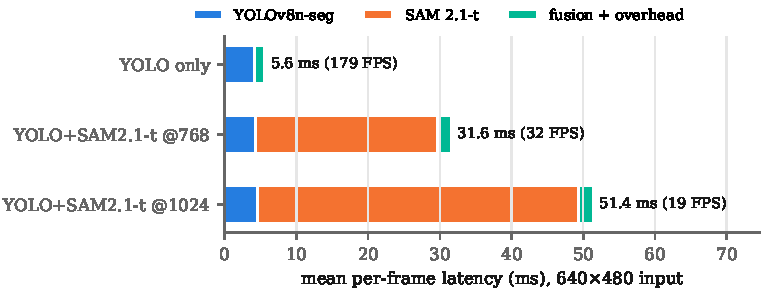
\includegraphics[width=0.78\textwidth]{seg_benchmark.pdf}
\caption{Latency breakdown of the hybrid segmenter on the RTX~4050 Laptop GPU.}
\label{fig:segbench}
\end{figure}

\paragraph{Findings} SAM takes 80--87\% of the frame time. At \SI{768}{px} instead
of \SI{1024}{px} total latency drops 39\% to \SI{31.6}{\milli\second} (32\,FPS), double
the vehicle's \SI{15}{\hertz} camera, so perception is not the bottleneck. This agrees
with our earlier drone-feed measurements (\SI{36}{\milli\second} and
\SI{50}{\milli\second}). Run-to-run SD was below \SI{1}{\milli\second}.

\paragraph{Qualitative output} \Cref{fig:seg} shows hybrid segmentation of a laboratory
scene captured through the vehicle's camera stream. A partly visible object at the left edge is
wrongly labelled \emph{car} (0.45), and the chairs have only moderate confidence
(0.40--0.74). With the camera obstructed (c) the pipeline correctly returns nothing,
illustrating the visual channel's dependence on a clear view.

\begin{figure}[H]
\centering
\begin{subfigure}[t]{0.32\textwidth}
  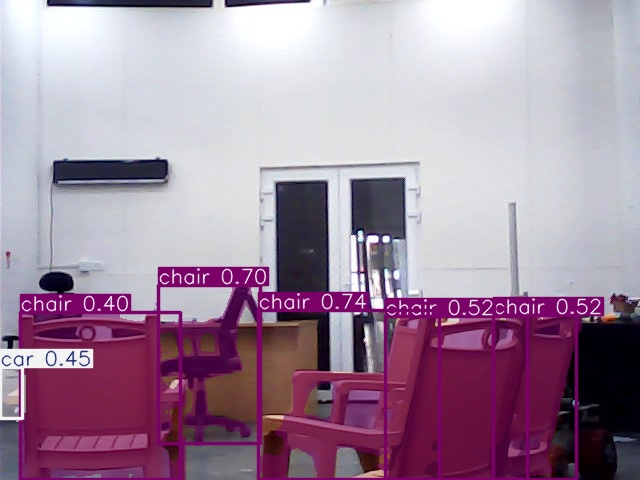
\includegraphics[width=\linewidth]{segmented_result.jpg}
  \caption{Annotated detections.}
\end{subfigure}\hfill
\begin{subfigure}[t]{0.32\textwidth}
  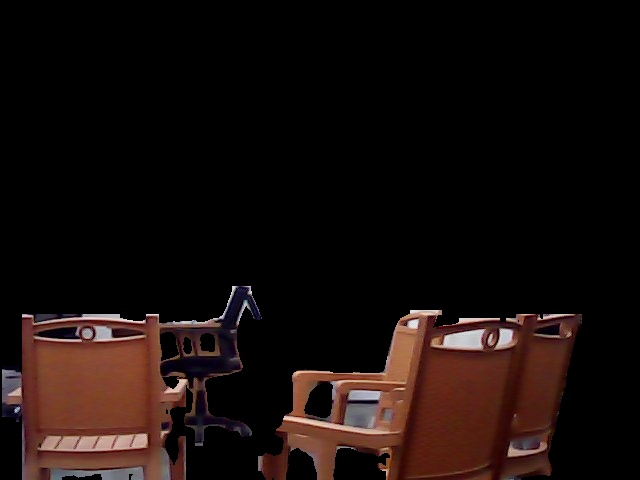
\includegraphics[width=\linewidth]{mask_overlay.jpg}
  \caption{Foreground masks only.}
\end{subfigure}\hfill
\begin{subfigure}[t]{0.32\textwidth}
  
\includegraphics[width=\linewidth]{received_raw_matrix.jpg}
  \caption{Obstructed camera frame.}
\end{subfigure}
\caption{Perception outputs saved by our stand-alone tools
(\code{live_segmentation.py --verify}, \code{camera_receiver.py}) from the vehicle's
camera stream (640$\times$480).}
\label{fig:seg}
\end{figure}

\subsection{Communication link}
\label{sec:val-link}

\Cref{tab:latency} gives our before/after latencies for the changes in
\cref{sec:design-link}. They were measured on one machine, so they isolate software
and queueing delay and exclude Wi-Fi air time; over-the-air latency is not yet
recorded, though the metrics of \cref{eq:latency} are in place.

\begin{table}[H]
\centering\small
\caption{Software-path latency before and after optimisation (project measurement,
single host; Wi-Fi time excluded).}
\label{tab:latency}
\begin{tabularx}{\textwidth}{l l l L}
\toprule
\textbf{Path} & \textbf{Before} & \textbf{After} & \textbf{Main change} \\
\midrule
Pixhawk $\rightarrow$ telemetry sent & \SI{28}{\milli\second} (up to 100) & \SI{5}{\milli\second} & 30\,Hz message intervals, event-driven send \\
Telemetry $\rightarrow$ \topic{/odom} & \SI{20}{\milli\second} @ 10\,Hz & \SI{2}{\milli\second} @ 30\,Hz & publish on arrival, drain backlog \\
\topic{/cmd_vel} $\rightarrow$ Pixhawk & \SI{54}{\milli\second} (up to 100) & \SI{1.4}{\milli\second} & forward on arrival, wake listener \\
\bottomrule
\end{tabularx}
\end{table}

\begin{figure}[H]
\centering
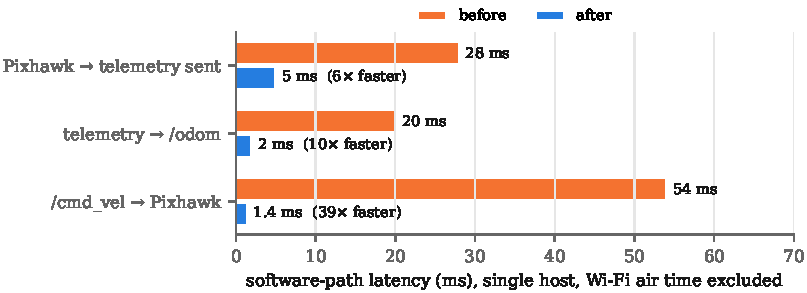
\includegraphics[width=0.78\textwidth]{link_latency.pdf}
\caption{Software-path latency before and after the link optimisations
(\cref{tab:latency}); the command path is 39 times faster.}
\label{fig:latency}
\end{figure}

Nominal rates on the vehicle are \topic{/odom} $\approx$\SI{30}{\hertz},
\topic{/scan} $\approx$\SI{7}{\hertz} (6.4\,rev/s) and camera $\approx$\SI{15}{\hertz}.
Sleeping to enforce the telemetry rate cap delayed fresh bursts by
\SI{15}{\milli\second} (median), so the streamer now skips early sends instead
(\cref{fig:flow-telemetry}). By \cref{eq:frag}, at 5\% fragment loss the
single-datagram LiDAR encoding is delivered with probability 0.95, against 0.86 for the
three-fragment JSON scan.

\subsection{Real-vehicle flight tests}
\label{sec:val-hwdemo}

\paragraph{Hover drift} The vehicle held position in \code{GUIDED} mode, with no GNSS,
for \SI{7}{\minute} at \SI{2.5}{\metre} above a grass surface, using the optical-flow
and rangefinder reference. Drift was measured against marks on the ground with a tape
and the flight video. The total
horizontal drift was \SI{1.6}{\metre}, i.e.\ about \SI{0.23}{\metre\per\minute}.
This is roughly ten times better than the $\ge$\SI{2}{\metre\per\minute} typical of
GNSS-free fallback (\cref{tab:kpi}) and bounded, unlike the inertial-only solution
(\SI{86.5}{\metre} in \SI{25}{\second}, \cref{sec:val-dr}). It is still over 30
times the \SI{5}{\centi\metre}/\SI{10}{\minute} KPI, even over a shorter window. A single run with tape-and-video
ground truth gives the order of magnitude, not a statistical figure.
\Cref{fig:driftcmp} places the hover result beside the inertial-only drift measured on
the same autopilot.

\begin{figure}[H]
\centering
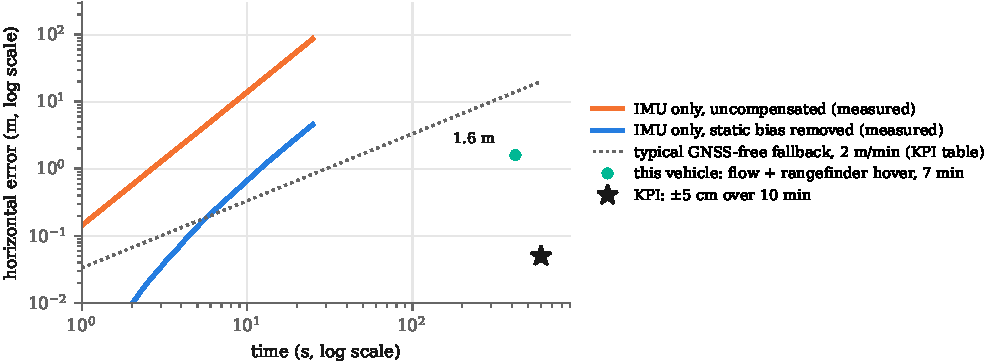
\includegraphics[width=0.92\textwidth]{drift_comparison.pdf}
\caption{Horizontal position error against time (log--log). Inertial-only curves are
from the stationary bench log (\cref{sec:val-dr}); the green point is the
\SI{7}{\minute} flow-and-rangefinder hover at \SI{2.5}{\metre} over grass (only the end
point was measured). The dotted line is the typical GNSS-free fallback and the star the
hover-drift KPI.}
\label{fig:driftcmp}
\end{figure}

\paragraph{Autonomous square path with obstacle avoidance} In a second flight, recorded
outdoors at night (\url{https://youtu.be/y1GYuHiDs4U}, \cref{fig:hwdemo}), Nav2 flew
the vehicle autonomously in \code{GUIDED} mode around a square path among trees, with
the pilot only taking off, landing and standing by. LiDAR returns from trunks and
foliage appear as lethal cells with an inflation layer in the live costmap, and the
planner routed the vehicle around them. The flight shows the complete closed loop on
hardware: sensing on the Pi, the Wi-Fi link, odometry, costmaps, planning and gated
velocity commands back to the autopilot, without ambient light. The video has no
external position reference, so path-following error and avoidance success rate are
not quantified.

\begin{figure}[H]
\centering
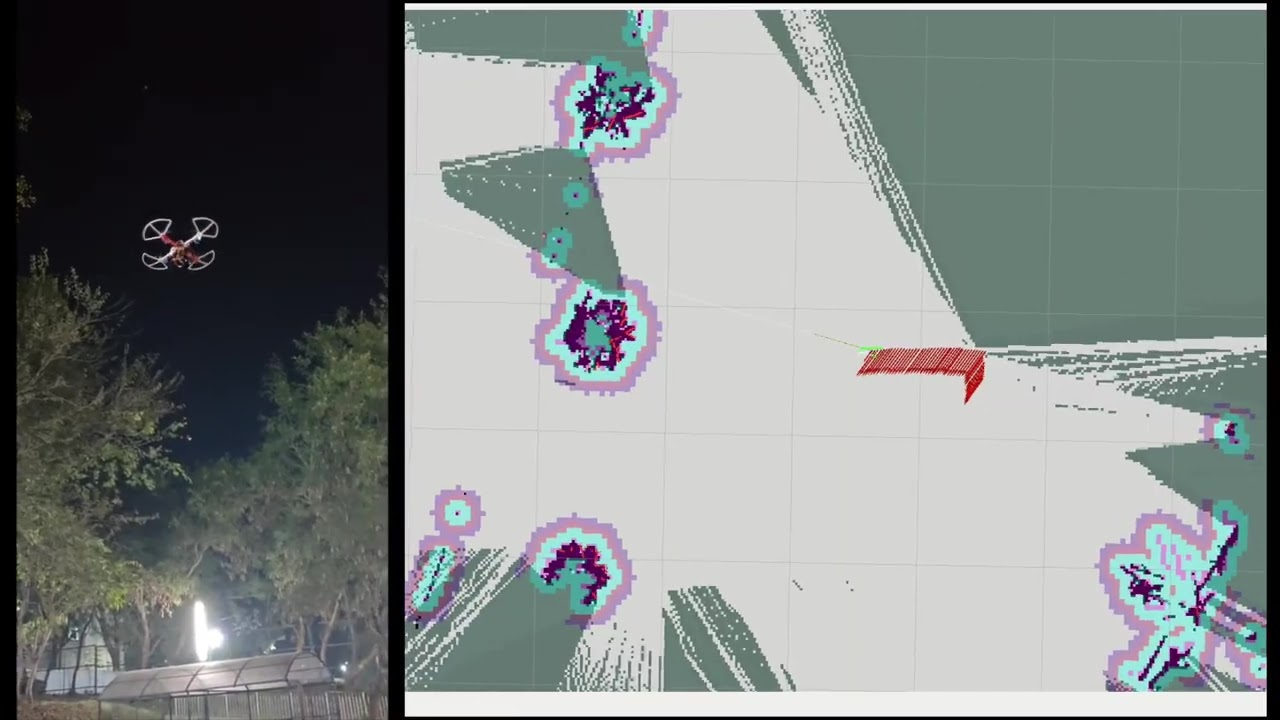
\includegraphics[width=\textwidth]{hardware_demo.jpg}
\caption{Autonomous square-path flight with obstacle avoidance (outdoors, at
night). Left: the quadcopter in flight. Right: live RViz view on the ground computer with LiDAR-derived obstacles
(trees) and their inflated Nav2 costmap, and the vehicle's estimated pose (red). Frame
from the video at \url{https://youtu.be/y1GYuHiDs4U}.}
\label{fig:hwdemo}
\end{figure}

\subsection{Simulation}

In the office world the vehicle explores autonomously until no frontier remains,
then returns to the start. \Cref{fig:sim} shows a frame of a recorded run
(\code{sim_office.launch.py}, video at \url{https://youtu.be/bwV-gUs8EIc}): mapped
free space is confined to rooms already observed, showing frontier-driven coverage.

\begin{figure}[H]
\centering
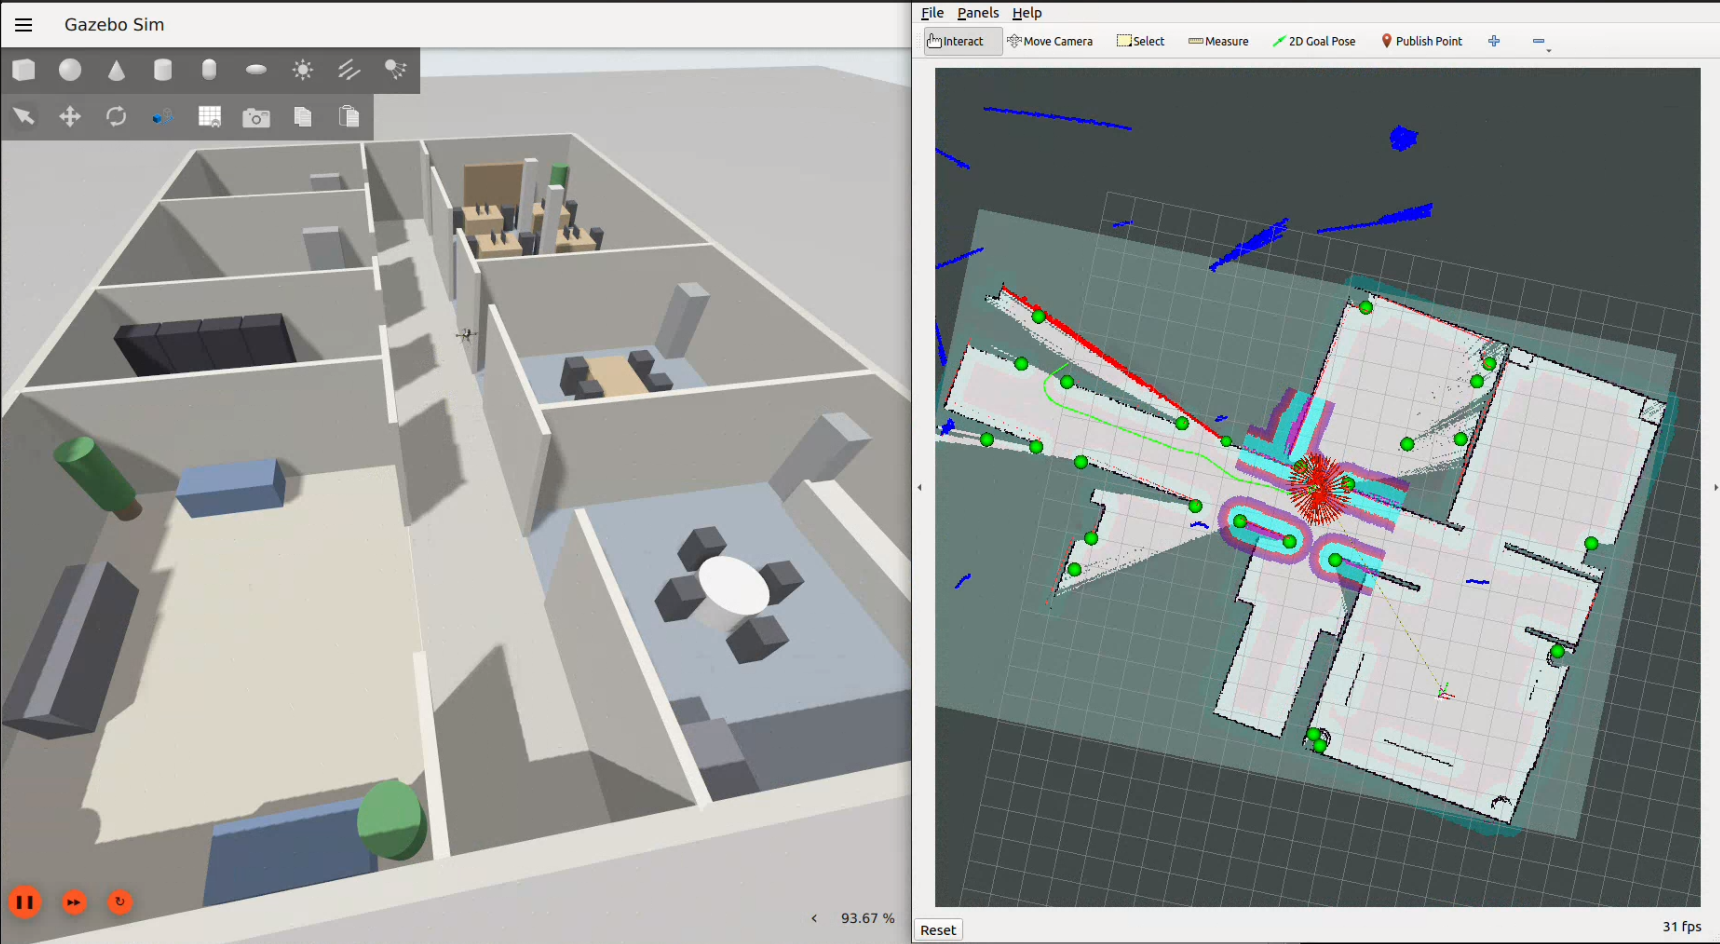
\includegraphics[width=\textwidth]{sim.png}
\caption{Autonomous exploration in the simulated office world (PX4 SITL, Gazebo
Harmonic, ROS~2). Left: Gazebo scene with the x500 in the corridor. Right: RViz with the
SLAM map, inflated costmaps, LiDAR scan, frontier markers (green) and planned path.
Video of the full run: \url{https://youtu.be/bwV-gUs8EIc}.}
\label{fig:sim}
\end{figure}

Simulation also shaped the design: the custom behaviour tree, the projection-based
safety filter (\cref{sec:design-safety}) and a single-instance guard against
\code{TF_OLD_DATA} floods all came from failures observed here.

\subsection{Quantitative analysis of the simulation flight logs}
\label{sec:val-simlogs}

\paragraph{Data} A development session on 20 November 2026 left 34 PX4 ULog files;
26 contain at least \SI{30}{s} armed in \code{OFFBOARD}, totalling \SI{6213}{s}
(\SI{1.7}{h}): 9 office and 17 Baylands flights (six from the open-field spawn).
\code{report/scripts/extract_sim_logs.py} extracts Gazebo ground truth, the EKF2
estimate, the velocity setpoints, the LiDAR scan as PX4 sees it (72 sectors of
\ang{5}) and the flight mode, resampled to \SI{5}{Hz}; \code{make_sim_figures.py}
computes every number below. \code{explore_lite} logs give each exploration's start,
end and termination reason.

Statistics run from \SI{15}{s} after \code{OFFBOARD} starts (excluding take-off) to its
end, or to \SI{2}{s} before the first \emph{fall} (dropping below \SI{0.5}{m} while
commanded higher). Caveats: the software changed between runs; EKF2 fused simulated GPS
in all runs (\code{EKF2_GPS_CTRL}${}=7$), so estimator errors are GPS-aided; and
Gazebo's sensors are idealised.

\paragraph{Sensor model check} To check the data path and frame conventions, every
LiDAR return of one complete exploration was projected at the ground-truth pose into
\SI{10}{cm} cells (\cref{fig:simmap}a). 78\% of cells hit 20 or more times lie within
\SI{0.15}{m} of an object reaching the scan plane; furniture below the plane leaves no
returns, as designed (\cref{sec:op-sim}).

\begin{figure}[p]
\centering
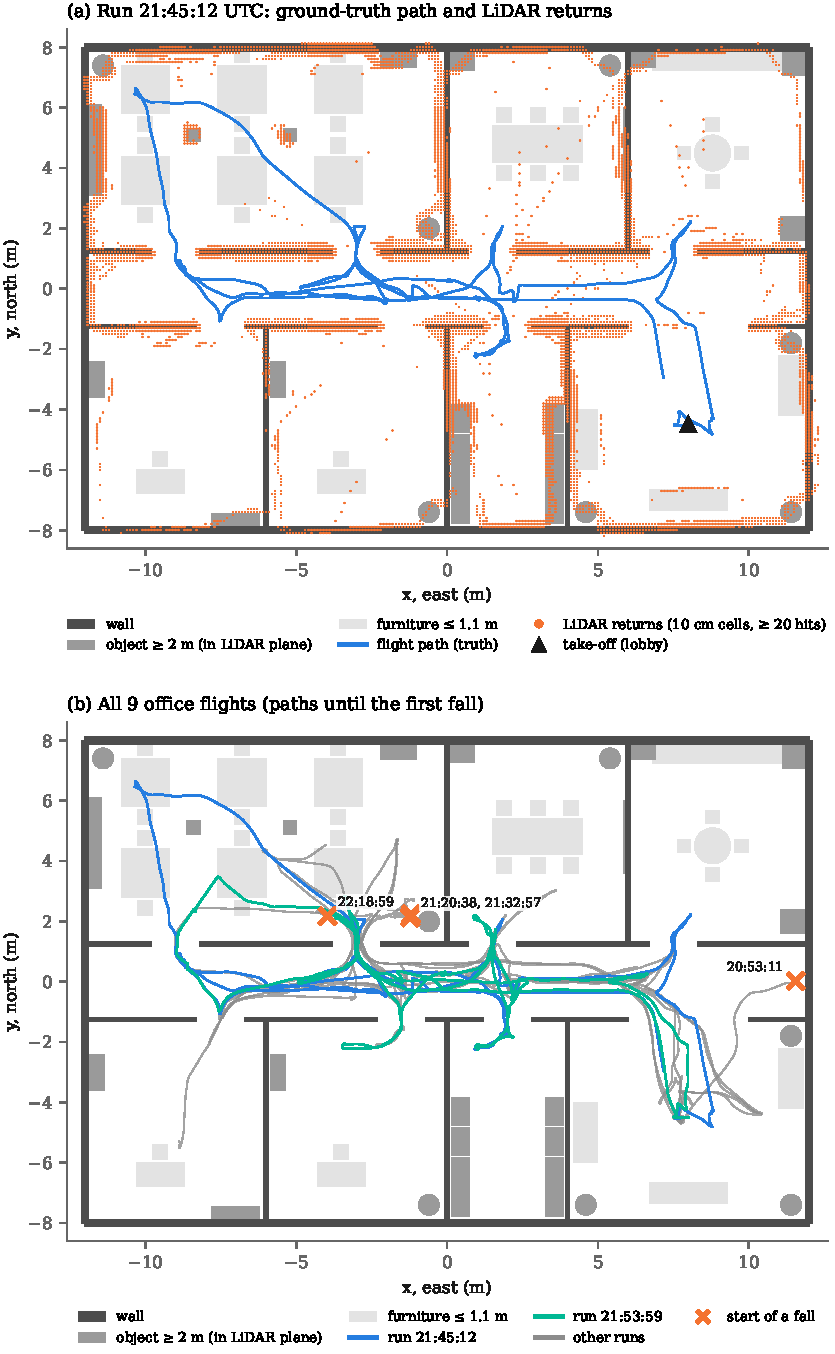
\includegraphics[width=0.84\textwidth]{sim_office_map.pdf}
\caption{Office world, top view (from \code{office.sdf}).
(a)~Run 21:45:12~UTC, a complete autonomous exploration: ground-truth flight path
and the LiDAR returns accumulated at the ground-truth pose.
(b)~All nine office flights, with each path shown until its first fall; crosses mark
where a fall began (\cref{tab:simincidents}).}
\label{fig:simmap}
\end{figure}

\paragraph{Exploration} Three of the office flights ended with \code{explore_lite}
reporting that all frontiers had been traversed or tried, after which the vehicle
returned towards the lobby:
\begin{itemize}[nosep]
  \item 21:45:12 explored for \SI{414}{s} and flew \SI{105.5}{m} with no fall;
  \item 21:53:59 explored for \SI{488}{s} and flew \SI{98.6}{m} with no fall;
  \item 21:32:57 explored for \SI{480}{s}; it fell once, climbed back and carried on.
\end{itemize}
Run 21:45:12 (\cref{fig:simmap}a, \cref{fig:simts}) visited every room except
office~A, which it mapped through the doorway. \Cref{tab:simruns} lists all office
flights and the Baylands flights longer than \SI{10}{m}.

\begin{table}[t]
\centering\footnotesize
\setlength{\tabcolsep}{3.2pt}
\caption{Simulation flights (PX4 SITL + Gazebo; truth from Gazebo). Height: error of
the height above the floor against the commanded height. Speed: horizontal, truth.
Track: RMS of commanded minus estimated velocity. Clear.: nearest LiDAR return.
$<$0.65: share of time inside the bridge's stop distance. Est.: EKF2 horizontal error,
\textbf{GPS-aided}. Baylands*: open-field spawn.}
\label{tab:simruns}
% generated by report/scripts/make_sim_figures.py from sim_runs.csv - do not edit
\begin{tabular}{@{}l l r r r r r r r r r r l@{}}
\toprule
& & \multicolumn{1}{c}{\textbf{OFFB.}} & \multicolumn{1}{c}{\textbf{Path}} &
\multicolumn{2}{c}{\textbf{Height (cm)}} & \multicolumn{2}{c}{\textbf{Speed (m/s)}} &
\multicolumn{1}{c}{\textbf{Track}} & \multicolumn{1}{c}{\textbf{Clear.}} &
\multicolumn{1}{c}{\textbf{$<$0.65}} & \multicolumn{1}{c}{\textbf{Est.}} & \\
\cmidrule(lr){5-6}\cmidrule(lr){7-8}
\textbf{Run (UTC)} & \textbf{World} & (s) & (m) & RMS & max & mean & p95 & (m/s) &
min (m) & (\%) & (cm) & \textbf{Outcome} \\
\midrule
19:09:55 & Baylands* & 182 & 13.5 & 6 & 21 & 0.08 & 0.91 & 0.07 & 16.54 & 0.0 & 4.3 & goals by operator \\
19:19:41 & Baylands* & 235 & 53.0 & 8 & 12 & 0.23 & 0.93 & 0.14 & 0.86 & 0.0 & 7.0 & goals by operator \\
19:28:09 & Baylands* & 429 & 194.0 & 4 & 24 & 0.47 & 0.94 & 0.20 & 0.71 & 0.0 & 18.4 & goals by operator \\
19:49:03 & Baylands & 225 & 43.3 & 6 & 14 & 0.20 & 0.94 & 0.17 & 1.70 & 0.0 & 6.6 & goals by operator \\
20:16:15 & Baylands & 52 & 18.5 & 4 & 17 & 0.46 & 0.99 & 0.49 & 0.39 & 5.9 & 7.8 & goals by operator \\
20:20:36 & Baylands & 533 & 97.5 & 6 & 32 & 0.19 & 0.92 & 0.14 & 0.81 & 0.0 & 5.5 & goals by operator \\
20:49:32 & Office & 137 & 19.9 & 3 & 6 & 0.16 & 0.51 & 0.07 & 0.53 & 13.3 & 4.0 & goals by operator \\
20:53:11 & Office & 370 & 8.6 & 5 & 9 & 0.04 & 0.44 & 0.03 & 0.62 & 0.2 & 3.9 & fall at 230\,s \\
21:00:33 & Office & 196 & 34.0 & 3 & 8 & 0.18 & 0.50 & 0.07 & 0.44 & 12.4 & 5.4 & goals by operator \\
21:04:15 & Baylands & 53 & 31.6 & 4 & 9 & 0.81 & 0.98 & 0.49 & 0.96 & 0.0 & 7.6 & goals by operator \\
21:20:38 & Office & 622 & 64.2 & 4 & 8 & 0.37 & 0.52 & 0.24 & 0.43 & 28.9 & 5.5 & exploring, stopped; fall at 185\,s \\
21:32:57 & Office & 686 & 77.4 & 3 & 20 & 0.30 & 0.51 & 0.23 & 0.59 & 2.3 & 5.3 & explored, all frontiers; fall at 266\,s \\
21:45:12 & Office & 465 & 105.5 & 11 & 47 & 0.23 & 0.51 & 0.13 & 0.62 & 0.4 & 4.6 & explored, all frontiers \\
21:53:59 & Office & 528 & 98.6 & 10 & 45 & 0.19 & 0.50 & 0.12 & 0.62 & 0.1 & 4.1 & explored, all frontiers \\
22:05:42 & Office & 232 & 60.3 & 12 & 42 & 0.27 & 0.52 & 0.15 & 0.66 & 0.0 & 6.5 & exploring, stopped \\
22:18:59 & Office & 118 & 28.0 & 14 & 34 & 0.28 & 0.49 & 0.18 & 0.61 & 2.4 & 3.4 & explored, no frontiers; fall at 108\,s \\
\bottomrule
\end{tabular}

\end{table}

\begin{figure}[t]
\centering
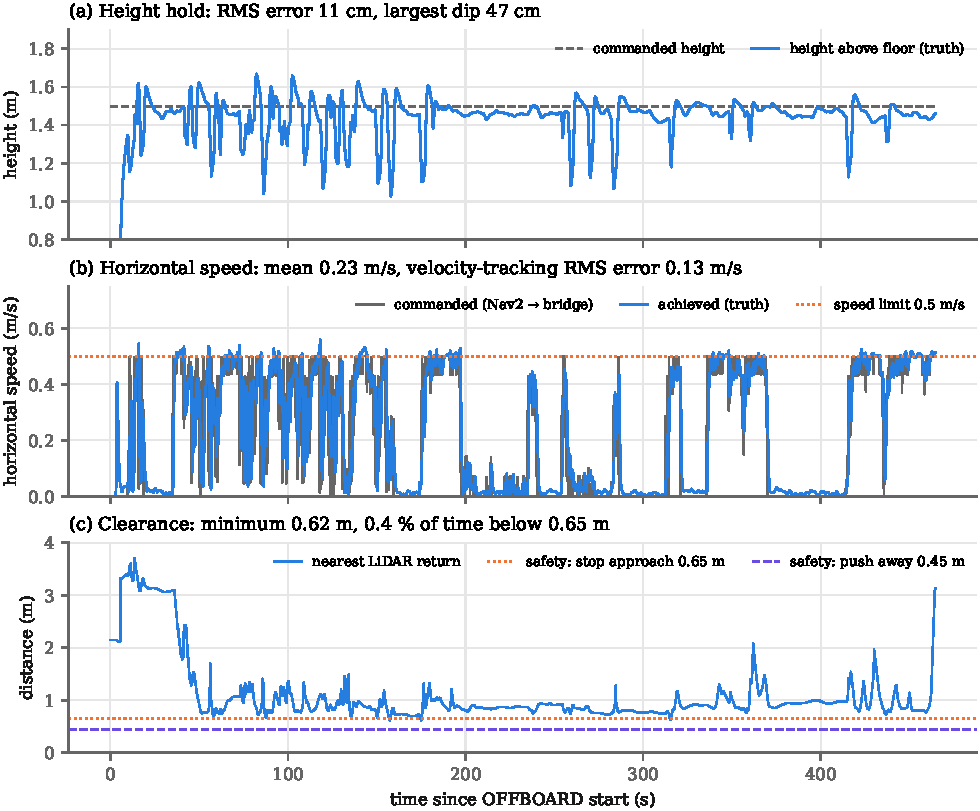
\includegraphics[width=\textwidth]{sim_office_timeseries.pdf}
\caption{Complete office exploration, run 21:45:12~UTC: (a) height above the floor
against the \SI{1.5}{m} command; (b) commanded and achieved horizontal speed against
the \SI{0.5}{m/s} limit; (c) nearest LiDAR return against the bridge's two safety
distances.}
\label{fig:simts}
\end{figure}

\paragraph{Speed and command tracking} Commanded speed never exceeded the configured
limits (\SI{0.5}{m/s} office, \SI{1.0}{m/s} Baylands); the true 95th percentile was at
most \SI{0.52}{m/s} and \SI{0.99}{m/s}. Velocity tracking error was 0.12--\SI{0.24}{m/s}
RMS, mostly at abrupt goal changes (\cref{fig:simts}b). Speed is bimodal
(\cref{fig:simclear}b): hovering while planning, and cruising at the limit.

\paragraph{Height hold} RMS height error was 3--\SI{14}{cm}. Later flights (21:45
onwards) dip up to \SI{47}{cm} when braking, recovering in about \SI{3}{s}
(\cref{fig:simts}a). These dips are a real risk: the office has no furniture between \SI{1.1}{m} and
\SI{2.0}{m}, where the LiDAR plane sits (\cref{sec:op-sim}), and a dip takes the vehicle
into the band of unseen low furniture, as in the 22:18:59 fall.

\paragraph{Clearance} In the two clean explorations the nearest return never fell
below \SI{0.62}{m}; it was inside the \SI{0.65}{m} stop distance 0.4\% and 0.1\% of the
time and never inside \SI{0.45}{m} (\cref{fig:simclear}a). Earlier flights spent
12--13\% (and 21:20:38, before its fall, 29\%) inside \SI{0.65}{m}, e.g.\ at doorways.

\begin{figure}[t]
\centering
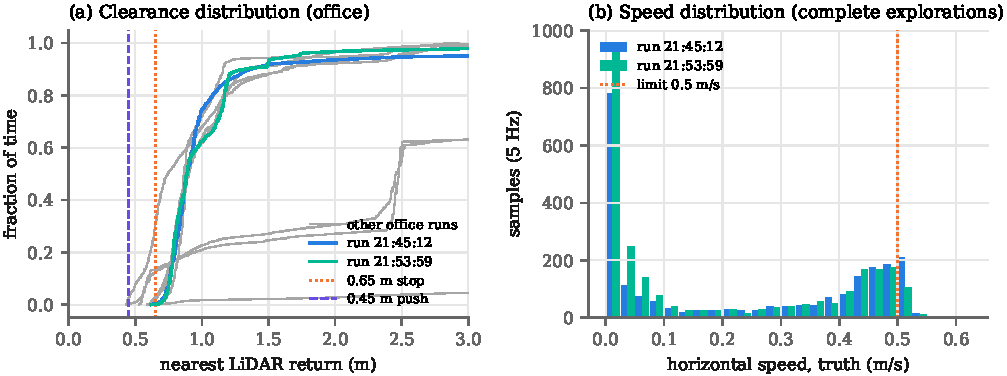
\includegraphics[width=\textwidth]{sim_clearance_speed.pdf}
\caption{(a) Cumulative distribution of the nearest LiDAR return over all office
flights, each up to its first fall. (b) Horizontal speed distribution of the two
complete explorations without a fall.}
\label{fig:simclear}
\end{figure}

\paragraph{Falls} Four office flights contain a fall (\cref{tab:simincidents},
crosses in \cref{fig:simmap}b), each 0.11--\SI{0.31}{m} from the nearest object, well
inside the x500's \SI{0.38}{m} propeller radius, so propeller contact is the likely
cause. The objects were the corridor end wall (20:53:11), the same potted plant at the
open-plan doorway (21:20:38, 21:32:57; later explorations passed it cleanly), and a
\SI{0.95}{m} chair below the LiDAR plane, reached after the vehicle sagged from
\SI{1.6}{m} to \SI{0.9}{m} (22:18:59). At the end wall the nearest return was
\SI{0.62}{m}, more than the true distance, for reasons the logs do not show. The vehicle
recovered height after every fall, and 21:32:57 went on to complete its exploration. One
Baylands log (20:16:15) ends \SI{0.2}{s} after a sudden \SI{5}{m/s} movement; a
collision is possible but unconfirmed and not counted.

\begin{table}[t]
\centering\footnotesize
\caption{Falls in the office flights. Time: since \code{OFFBOARD} start, when the height
began to drop. Position: Gazebo $x$ (east), $y$ (north). Distance: from the vehicle's
centre to the nearest object of \code{office.sdf}. LiDAR: nearest return in the 3\,s
before.}
\label{tab:simincidents}
% generated by report/scripts/make_sim_figures.py from sim_runs.csv - do not edit
\begin{tabular}{@{}l r l l r r l@{}}
\toprule
\textbf{Run (UTC)} & \textbf{Time (s)} & \textbf{Position (m)} & \textbf{Nearest object} &
\textbf{Dist.\ (m)} & \textbf{LiDAR (m)} & \textbf{Afterwards} \\
\midrule
20:53:11 & 230.4 & (11.56, 0.02) & wall, top 3.00\,m & 0.31 & 0.62 & climbed back; goals by operator \\
21:20:38 & 184.8 & (-1.22, 2.13) & plant, top 2.00\,m & 0.28 & 0.19 & climbed back; stopped by operator \\
21:32:57 & 266.1 & (-1.19, 2.23) & plant, top 2.00\,m & 0.28 & 0.42 & climbed back; exploration completed \\
22:18:59 & 107.7 & (-3.96, 2.17) & chair, top 0.95\,m & 0.11 & 0.72 & climbed back; no frontiers left \\
\bottomrule
\end{tabular}

\end{table}

\paragraph{Baylands} \Cref{fig:simbay}a shows the longest Baylands flight with goals
from the operator (\SI{533}{s} in \code{OFFBOARD}, \SI{97.5}{m}). The tree crowns appear
as clusters of LiDAR returns in the scan plane. The flight passes between them with a
minimum clearance of \SI{0.81}{m}.

Over all flights longer than \SI{5}{m}, EKF2's horizontal RMS error against ground
truth is at most \SI{18}{cm} (maximum \SI{36}{cm}; \cref{fig:simbay}b). Being
GPS-aided, this shows only that Nav2 received a consistent pose.

\begin{figure}[t]
\centering
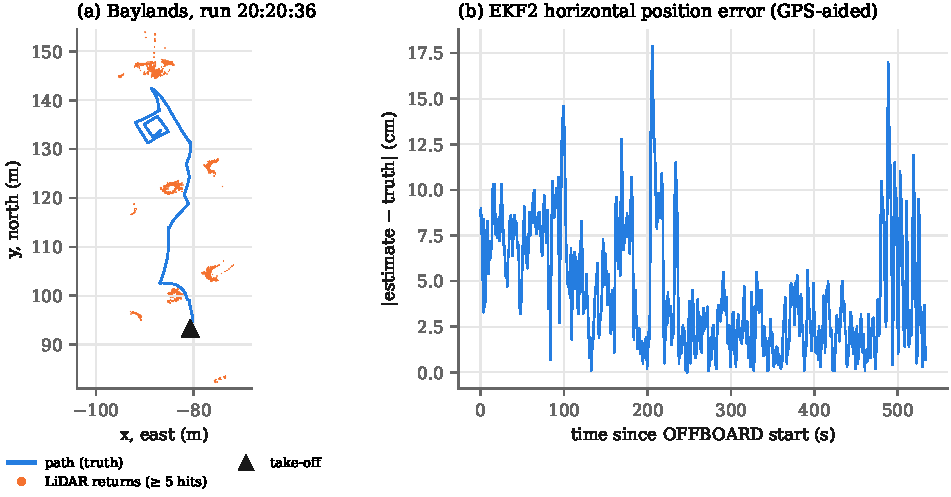
\includegraphics[width=\textwidth]{sim_baylands.pdf}
\caption{Baylands, run 20:20:36~UTC: (a) ground-truth path and accumulated LiDAR
returns (tree crowns in the scan plane); (b) horizontal error of EKF2's position
estimate against Gazebo truth, with simulated GPS fused.}
\label{fig:simbay}
\end{figure}

%% ---------------------------------------------------------------------
\section{Results, limitations and future improvements}
\label{sec:discussion}

\subsection{Summary of results}

\begin{itemize}[leftmargin=*,itemsep=1pt]
  \item \textbf{Real vehicle.} Nav2 flew an autonomous square path around trees,
    outdoors at night, and a \SI{7}{\minute} GNSS-free \code{GUIDED} hover at \SI{2.5}{\metre} over grass drifted
    \SI{1.6}{\metre} (\cref{sec:val-hwdemo}).
  \item \textbf{Simulation} (26 flights, \SI{1.7}{h}, Gazebo truth). Three complete
    office explorations (about \SI{100}{m} and 7--8 minutes each, two without contact);
    speed limits held (95th percentile $\le$\SI{0.52}{m/s}); height RMS 3--\SI{14}{cm}.
    Four falls exposed height sag when braking and too small a margin to the propellers
    (\cref{tab:simincidents}).
  \item \textbf{System.} LiDAR, flow odometry, Nav2, semantic perception and health
    monitoring added to an unmodified ArduPilot multirotor with USB-only connections;
    a five-layer safety-gated command path with pilot override.
  \item \textbf{Link.} Software-path latency reduced to single-digit milliseconds
    (\cref{tab:latency}), with fragmentation-free encodings and per-stream metrics.
  \item \textbf{Need for exteroception.} Inertial-only integration on real autopilot data
    drifted \SI{86.5}{\metre} in \SI{25}{\second} (\SI{4.6}{\metre} after bias removal);
    the ZUPT detector has an order-of-magnitude margin at rest.
  \item \textbf{Perception.} Hybrid YOLO--SAM runs at \SI{31.6}{\milli\second} per frame,
    twice the camera rate; 17/17 logic tests pass.
\end{itemize}

\subsection{Status against the KPIs}

\begin{table}[H]
\centering\small
\caption{Verification status of each KPI for the current prototype.}
\label{tab:kpistatus}
\begin{tabularx}{\textwidth}{p{2.8cm} p{3.2cm} L}
\toprule
\textbf{KPI} & \textbf{Status} & \textbf{Evidence / gap} \\
\midrule
Trajectory error $<0.5\%$ & Not measured & Requires flights with ground truth (motion capture, surveyed markers or total station). The trade study predicts 1.4--1.5\% for the prototype's sensing, i.e.\ above target \\
Hover drift $\le\pm$\SI{5}{\centi\metre}/\SI{10}{\minute} & Not met & \SI{1.6}{\metre} over \SI{7}{\minute} in flight (\cref{sec:val-hwdemo}); about 10$\times$ better than GNSS-free fallback, over 30$\times$ the target \\
State $\ge$\SI{100}{\hertz}, vision $\ge$\SI{30}{\hertz} & Partly & Ground \topic{/odom} $\approx$\SI{30}{\hertz} (autopilot EKF runs faster internally). Camera $\approx$\SI{15}{\hertz}, limited by the USB camera. Perception capacity 32\,FPS \\
Compute $\le$\SI{15}{\watt} onboard & Not met by design & Processing is off-board on a GPU laptop in the prototype \\
\SIrange{0}{10000}{lux} & Partly & LiDAR and flow-based navigation is illumination-independent by principle. Camera perception is not. Untested \\
Endurance $\ge$\SI{30}{\minute} & Not met & Target battery is recorded as $\approx$\SI{10}{\minute} \\
\bottomrule
\end{tabularx}
\end{table}

\begin{figure}[H]
\centering
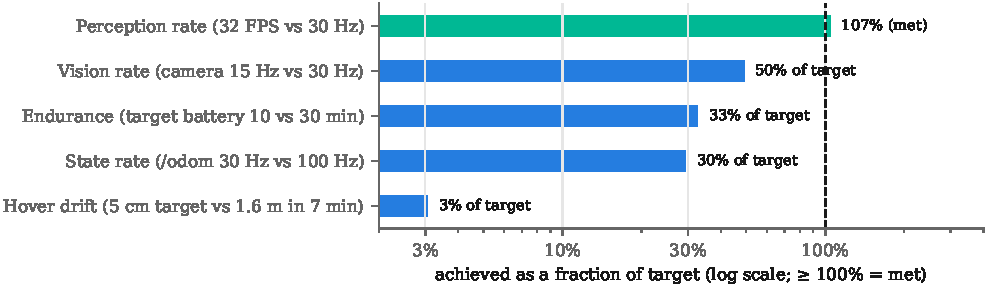
\includegraphics[width=0.85\textwidth]{kpi_status.pdf}
\caption{Measurable KPIs as a fraction of their targets (log scale). Trajectory error
(not yet measured), onboard compute (off-board by design) and illumination (untested)
are omitted. Hover drift is target over achieved, so 3\% means 32 times the
allowed drift.}
\label{fig:kpistatus}
\end{figure}

\subsection{Limitations}
\label{sec:limitations}

\begin{enumerate}[leftmargin=*,itemsep=2pt]
  \item \textbf{Limited flight validation on hardware.} This is the main gap. Our
    hover-drift figure (\SI{1.6}{\metre} in \SI{7}{\minute}) comes from a single run at
    \SI{2.5}{\metre} over grass, and the square-path flight had no external reference.
    We therefore cannot yet report trajectory error, avoidance success rate or
    over-the-air latency. The drift is also more than 30 times our KPI. We suspect the
    grass (its texture is low and repetitive, and it moves in the propeller downwash),
    the coarser flow resolution at \SI{2.5}{\metre}, and EKF tuning; repeating the test
    over a textured mat at \SIrange{1}{1.5}{\metre} should tell these apart. The
    simulation results (\cref{sec:val-simlogs}) use idealised sensors and cannot stand in
    for real flights.
  \item \textbf{Collision margin in simulation.} Four of nine simulated office flights
    contained a fall after propeller contact (\cref{tab:simincidents}). The bridge's
    \SI{0.65}{m} stop distance is measured from the LiDAR, while the propellers reach
    about \SI{0.38}{m} from the centre. Braking height dips of up to \SI{47}{cm} brought
    the vehicle down to the height of furniture the LiDAR cannot see. We need to fix both
    before flying the real vehicle indoors.
  \item \textbf{Off-board dependence.} Planning and perception require the Wi-Fi link.
    If the link drops, the
    stale-command stop and autopilot hold bring the vehicle to a safe halt, but the
    mission ends there. This is why the final design moves all processing onboard.
  \item \textbf{Odometry without loop closure.} On the real vehicle Nav2 runs in a
    rolling \code{odom} frame, and SLAM is used only in simulation. Flow-based
    dead-reckoning drifts with distance, and there is no covariance-weighted fusion of
    flow, LiDAR and IMU on the ground. The \code{/odom} covariance is not modelled.
  \item \textbf{2D sensing in a 3D world.} The LiDAR sees a single horizontal
    slice, so anything above or below it is invisible. We designed the simulated office
    around this limitation. The
    \code{scan_to_3d} map is built for inspection and does not feed the costmaps.
  \item \textbf{Placeholder extrinsics.} The LiDAR and camera mount transforms are
    estimates and must be calibrated for each build.
  \item \textbf{Optical-flow assumptions.} Conversion assumes a flat floor and correct
    \code{FLOW_ORIENT_YAW}. Flow quality falls over textureless or reflective floors,
    and samples below quality 20 are dropped, so velocity becomes zero.
  \item \textbf{Simulation--reality gap.} The simulation uses PX4 OFFBOARD with
    simulated GNSS in the estimator. The vehicle uses ArduPilot \code{GUIDED} without
    GNSS. The LiDAR safety filter exists only in the simulation bridge.
  \item \textbf{Screening estimates.} The trade-study figures are literature-typical
    values, not measurements.
\end{enumerate}

\subsection{Future improvements}

Ordered by our timeline (\cref{tab:timeline}) and by the gaps above:
\begin{enumerate}[leftmargin=*,itemsep=2pt]
  \item \textbf{Flight validation campaign.} Repeated hover-drift and figure-of-eight
    trajectory tests against an external reference. Report RMSE absolute trajectory
    error, drift as a percentage of distance, avoidance success rate, and the
    over-the-air latency distribution from \topic{/metrics/*/latency_ms}.
  \item \textbf{Fix the collision causes found in simulation.}
    \begin{itemize}[nosep]
      \item Measure the safety distances from the propeller envelope, not from the
        LiDAR.
      \item Hold height while braking.
      \item Add a regression test that replays the office exploration and fails on any
        fall (our log analysis already detects falls).
      \item Repeat the analysis with GPS disabled in EKF2, using SLAM or flow as the
        position source.
    \end{itemize}
  \item \textbf{Real-vehicle SLAM and fusion.} Run SLAM~Toolbox on the real scan stream
    to provide \code{map}$\rightarrow$\code{odom} and loop closure. Feed the resulting
    pose back to EKF3 as external navigation (MAVLink \code{VISION_POSITION_ESTIMATE}
    or \code{ODOMETRY}), so the autopilot's estimate is bounded and not only the
    planner's.
  \item \textbf{Port the LiDAR safety filter} from the simulation bridge to the Pi
    listener, so it acts even when the ground link is degraded.
  \item \textbf{Migrate onboard} to the design target. Use a Raspberry Pi~5 with stereo
    VIO (ORB-SLAM3 or VINS-Fusion), PX4 on the Kakute H7, and the existing link layer
    kept only for telemetry. Measure power against the \SI{15}{\watt} budget.
  \item \textbf{Perception on embedded hardware.} Measure YOLO-only and
    reduced-resolution SAM on the Pi~5 or an accelerator. Project segmentation masks
    into the costmap as a semantic layer.
  \item \textbf{Language-commanded navigation} (objective 11). A prototype
    (\code{scripts/context_learning.py}) already resolves object references against a
    JSON object list with an LLM. Integrate it with the semantic map, and validate
    every LLM-generated goal against the costmap before execution.
  \item \textbf{Degraded-condition tests}: darkness, smoke, glare, blocked camera, and
    saturated IMU (objectives 3 and 5).
  \item \textbf{Open-hardware completeness.} An archived release with DOI.
\end{enumerate}

\begin{table}[H]
\centering\small
\caption{Project timeline and status (\code{docs/TIMELINE.md}).}
\label{tab:timeline}
\begin{tabularx}{\textwidth}{l p{2.2cm} L}
\toprule
\textbf{Phase} & \textbf{Weeks} & \textbf{Scope (milestone)} \\
\midrule
0 Concept & done & Problem statement, 15-solution survey, scoring, design choice, BOM \\
1 Hardware & 1--3 & Procure target parts, PX4 on Kakute H7, test rig, ELRS and failsafes (manual flight) \\
2 Sensing & 3--6 & Stereo calibration, rectified images $\ge$\SI{30}{\hertz}, depth, IMU-only baseline \\
3 Estimation \& SLAM & 6--9 & VIO, EKF/factor-graph fusion, loop closure, KPI measurement (bounded drift) \\
4 Planning & 9--11 & Costmaps from depth, Nav2 tuning, static/dynamic avoidance \\
5 Language & 11--13 & LLM goal grounding with costmap validation (``go to the window'') \\
6 Full system & 13--16 & End-to-end GPS-free mission, degraded-condition tests, KPI sign-off \\
\bottomrule
\end{tabularx}
\end{table}

\noindent The prototype and simulation stack described here serve as our development
platform for phases 1--4. We expect the link, safety, planning and perception layers to
carry over to the onboard design largely unchanged.

%% ---------------------------------------------------------------------
\section*{Ethics statements}
This work involved no human or animal subjects and no data collected from social media
platforms.

\section*{Declaration of competing interest}
The authors declare that they have no known competing financial interests or
personal relationships that could have appeared to influence the work reported in this
paper.

\section*{Funding}
This work was funded by the Design Practicum course of the Indian Institute of
Technology Mandi.

\section*{Acknowledgements}
The authors thank the Indian Institute of Technology Mandi and its Design Practicum
course for their support, and acknowledge the open-source projects on which this system builds:
ROS~2, Nav2, SLAM~Toolbox, \code{m-explore-ros2}, ArduPilot, PX4, Gazebo, pymavlink,
OpenCV, Ultralytics YOLO and Meta's Segment Anything.

\section*{Data and code availability}
All source code, configuration and documentation are available at
\url{https://github.com/DEEPAKSINGLA-byte/gps-denied-vtol}. The bench telemetry log,
segmentation benchmark results and simulation flight data used in this paper are in the
repository's \code{report/data/} directory. A video of the real vehicle's autonomous square-path flight with obstacle avoidance is
available at \url{https://youtu.be/y1GYuHiDs4U}, a video of autonomous exploration in
the simulated office world at \url{https://youtu.be/bwV-gUs8EIc}, and a demonstration of the
segmentation pipeline at \url{https://youtu.be/XxDwwBQxVR0}.


\bibliographystyle{elsarticle-num}
\bibliography{references}

\appendix
%% ---------------------------------------------------------------------
\section{Interface reference}
\label{app:reference}

\begin{table}[H]
\centering\small
\caption{ROS~2 topics produced by the ground stack.}
\begin{tabularx}{\textwidth}{p{5.2cm} L}
\toprule
\textbf{Topic} & \textbf{Content} \\
\midrule
\topic{/odom}, TF \code{odom}$\rightarrow$\code{base_link} & Vehicle pose/twist (EKF local position if available, otherwise flow dead-reckoning) \\
\topic{/scan} & \code{LaserScan}, 360 readings at \SI{1}{\degree} \\
\topic{/camera/image_raw} & Camera image \\
\topic{/drone/optical_flow} & Raw flow and ground distance (debug) \\
\topic{/segmentation/detections} & Class, score and box per object \\
\topic{/segmentation/class_mask}, \topic{/instance_mask} & Per-pixel class id + 1 / instance index + 1 \\
\topic{/segmentation/image_annotated} & Annotated image (published only when subscribed) \\
\topic{/cmd_vel} & Nav2 velocity command \\
\topic{/map_3d} & Voxelised 3D point cloud (\code{PointCloud2}, \SI{1}{\hertz}) \\
\topic{/diagnostics}, \topic{/metrics/overlay}, \topic{/metrics/dashboard} & Health summary and RViz overlays \\
\bottomrule
\end{tabularx}
\end{table}

\begin{table}[H]
\centering\small
\caption{Health metrics published under \topic{/metrics/}.}
\begin{tabularx}{\textwidth}{p{6.6cm} L}
\toprule
\textbf{Metric} & \textbf{Meaning} \\
\midrule
\code{{lidar,telemetry,camera}/latency_ms} & One-way Pi$\rightarrow$laptop latency (\cref{eq:latency}), absolute once clocks are synced \\
\code{*/latency_excess_ms} & Latency above the 10\,s-window minimum (clock-independent) \\
\code{*/rate_hz}, \code{lidar/jitter_ms} & Arrival rate and inter-arrival jitter \\
\code{camera/{decode_ms,bandwidth_mbps,dropped_frames}} & Camera cost and load \\
\code{lidar/{nearest_obstacle_m,valid_ratio,tf_fail_ratio}} & LiDAR quality \\
\code{tf/odom_base_age_ms} & Age of the latest pose \\
\code{costmap/local/scan_agreement} & \Cref{eq:agreement}; $\approx$1 when costmap matches LiDAR \\
\code{costmap/{local,global}/{rate_hz,lethal_cells}} & Costmap update rate and obstacle count \\
\code{odom/{speed_mps,distance_from_start_m,path_length_m}} & Motion and drift indicators \\
\code{flow/{quality,ground_distance_m}} & Optical-flow sensor state \\
\code{nav/{cmd_vel_rate_hz,cmd_speed_mps,plan_length_m}} & Planner activity \\
\code{segmentation/{inference_ms,yolo_ms,sam_ms,sam_refined}} & Perception cost and output \\
\bottomrule
\end{tabularx}
\end{table}

\begin{table}[H]
\centering\small
\caption{Options of \code{start_streams.py} (companion).}
\begin{tabularx}{\textwidth}{p{4.6cm} p{3.2cm} L}
\toprule
\textbf{Option} & \textbf{Default} & \textbf{Effect} \\
\midrule
\emph{laptop IP} (positional) & SSH client / gateway & Destination of all streams \\
\code{--nav-cmds} & off & Enable Nav2 velocity forwarding (armed + GUIDED only) \\
\code{--no-telemetry/--no-lidar/--no-camera} & -- & Omit a stream \\
\code{--pixhawk-port} & \code{/dev/pixhawk} & Autopilot device \\
\code{--lidar-port}, \code{--lidar-baud} & \code{/dev/ttyUSB0}, 115200 & LiDAR serial \\
\code{--camera-device}, \code{--camera-size} & \code{/dev/camera}, 640x480 & Camera and resolution \\
\code{--fps}, \code{--quality} & 20, 70 & Camera rate, JPEG quality \\
\code{--camera-passthrough} & off & Forward camera MJPEG without re-encoding \\
\code{--rate} & 30 & Max telemetry rate (Hz) \\
\code{--keep-powersave}, \code{--no-time-sync} & off & Skip Wi-Fi power-save change / clock sync \\
\bottomrule
\end{tabularx}
\end{table}

\begin{table}[H]
\centering\small
\caption{Arguments of \code{navigation_real.launch.py} (ground).}
\begin{tabularx}{\textwidth}{p{3.4cm} p{3.6cm} L}
\toprule
\textbf{Argument} & \textbf{Default} & \textbf{Effect} \\
\midrule
\code{pi_ip} & \code{$GPS_DENIED_PI_IP} & Companion address for commands \\
\code{camera}, \code{segmentation} & true, true & Camera receiver; YOLO+SAM node \\
\code{seg_model}, \code{seg_sam_model} & \code{yolov8n-seg.pt}, \code{sam2.1_t.pt} & Weights (\code{none} disables SAM) \\
\code{seg_sam_imgsz} & 768 & SAM input size (1024 = sharpest) \\
\code{rviz}, \code{metrics}, \code{map3d} & true & Visualisation, health monitor, 3D mapper \\
\code{params_file} & \code{config/nav2_real.yaml} & Nav2 parameters \\
\code{use_sim_time} & false & Simulation clock \\
\bottomrule
\end{tabularx}
\end{table}

\section{Reproducing the validation figures}
\label{app:repro}

\begin{lstlisting}[language=bash]
cd gps-denied-vtol
# segmentation timing (needs CUDA GPU, ultralytics, weights in ros2_ws/)
python3 report/scripts/bench_segmentation.py --iters 100
# bench-log figures, ZUPT and dead-reckoning analysis
python3 report/scripts/make_figures.py      # writes report/figures/*.pdf, data/bench_stats.txt
python3 report/scripts/make_extra_figures.py # latency, delivery, drift and KPI summary figures
# segmentation unit tests
cd ros2_ws/src/quadcopter_perception
PYTEST_DISABLE_PLUGIN_AUTOLOAD=1 python3 -m pytest test/test_hybrid_segmenter.py
# trade-study charts
python3 scripts/analysis.py
\end{lstlisting}

\section{Additional trade-study views}
\label{app:trade}

Cost and robustness views of the screening data in \cref{tab:solutions}.

\begin{figure}[H]
\centering
\begin{subfigure}[t]{0.49\textwidth}
  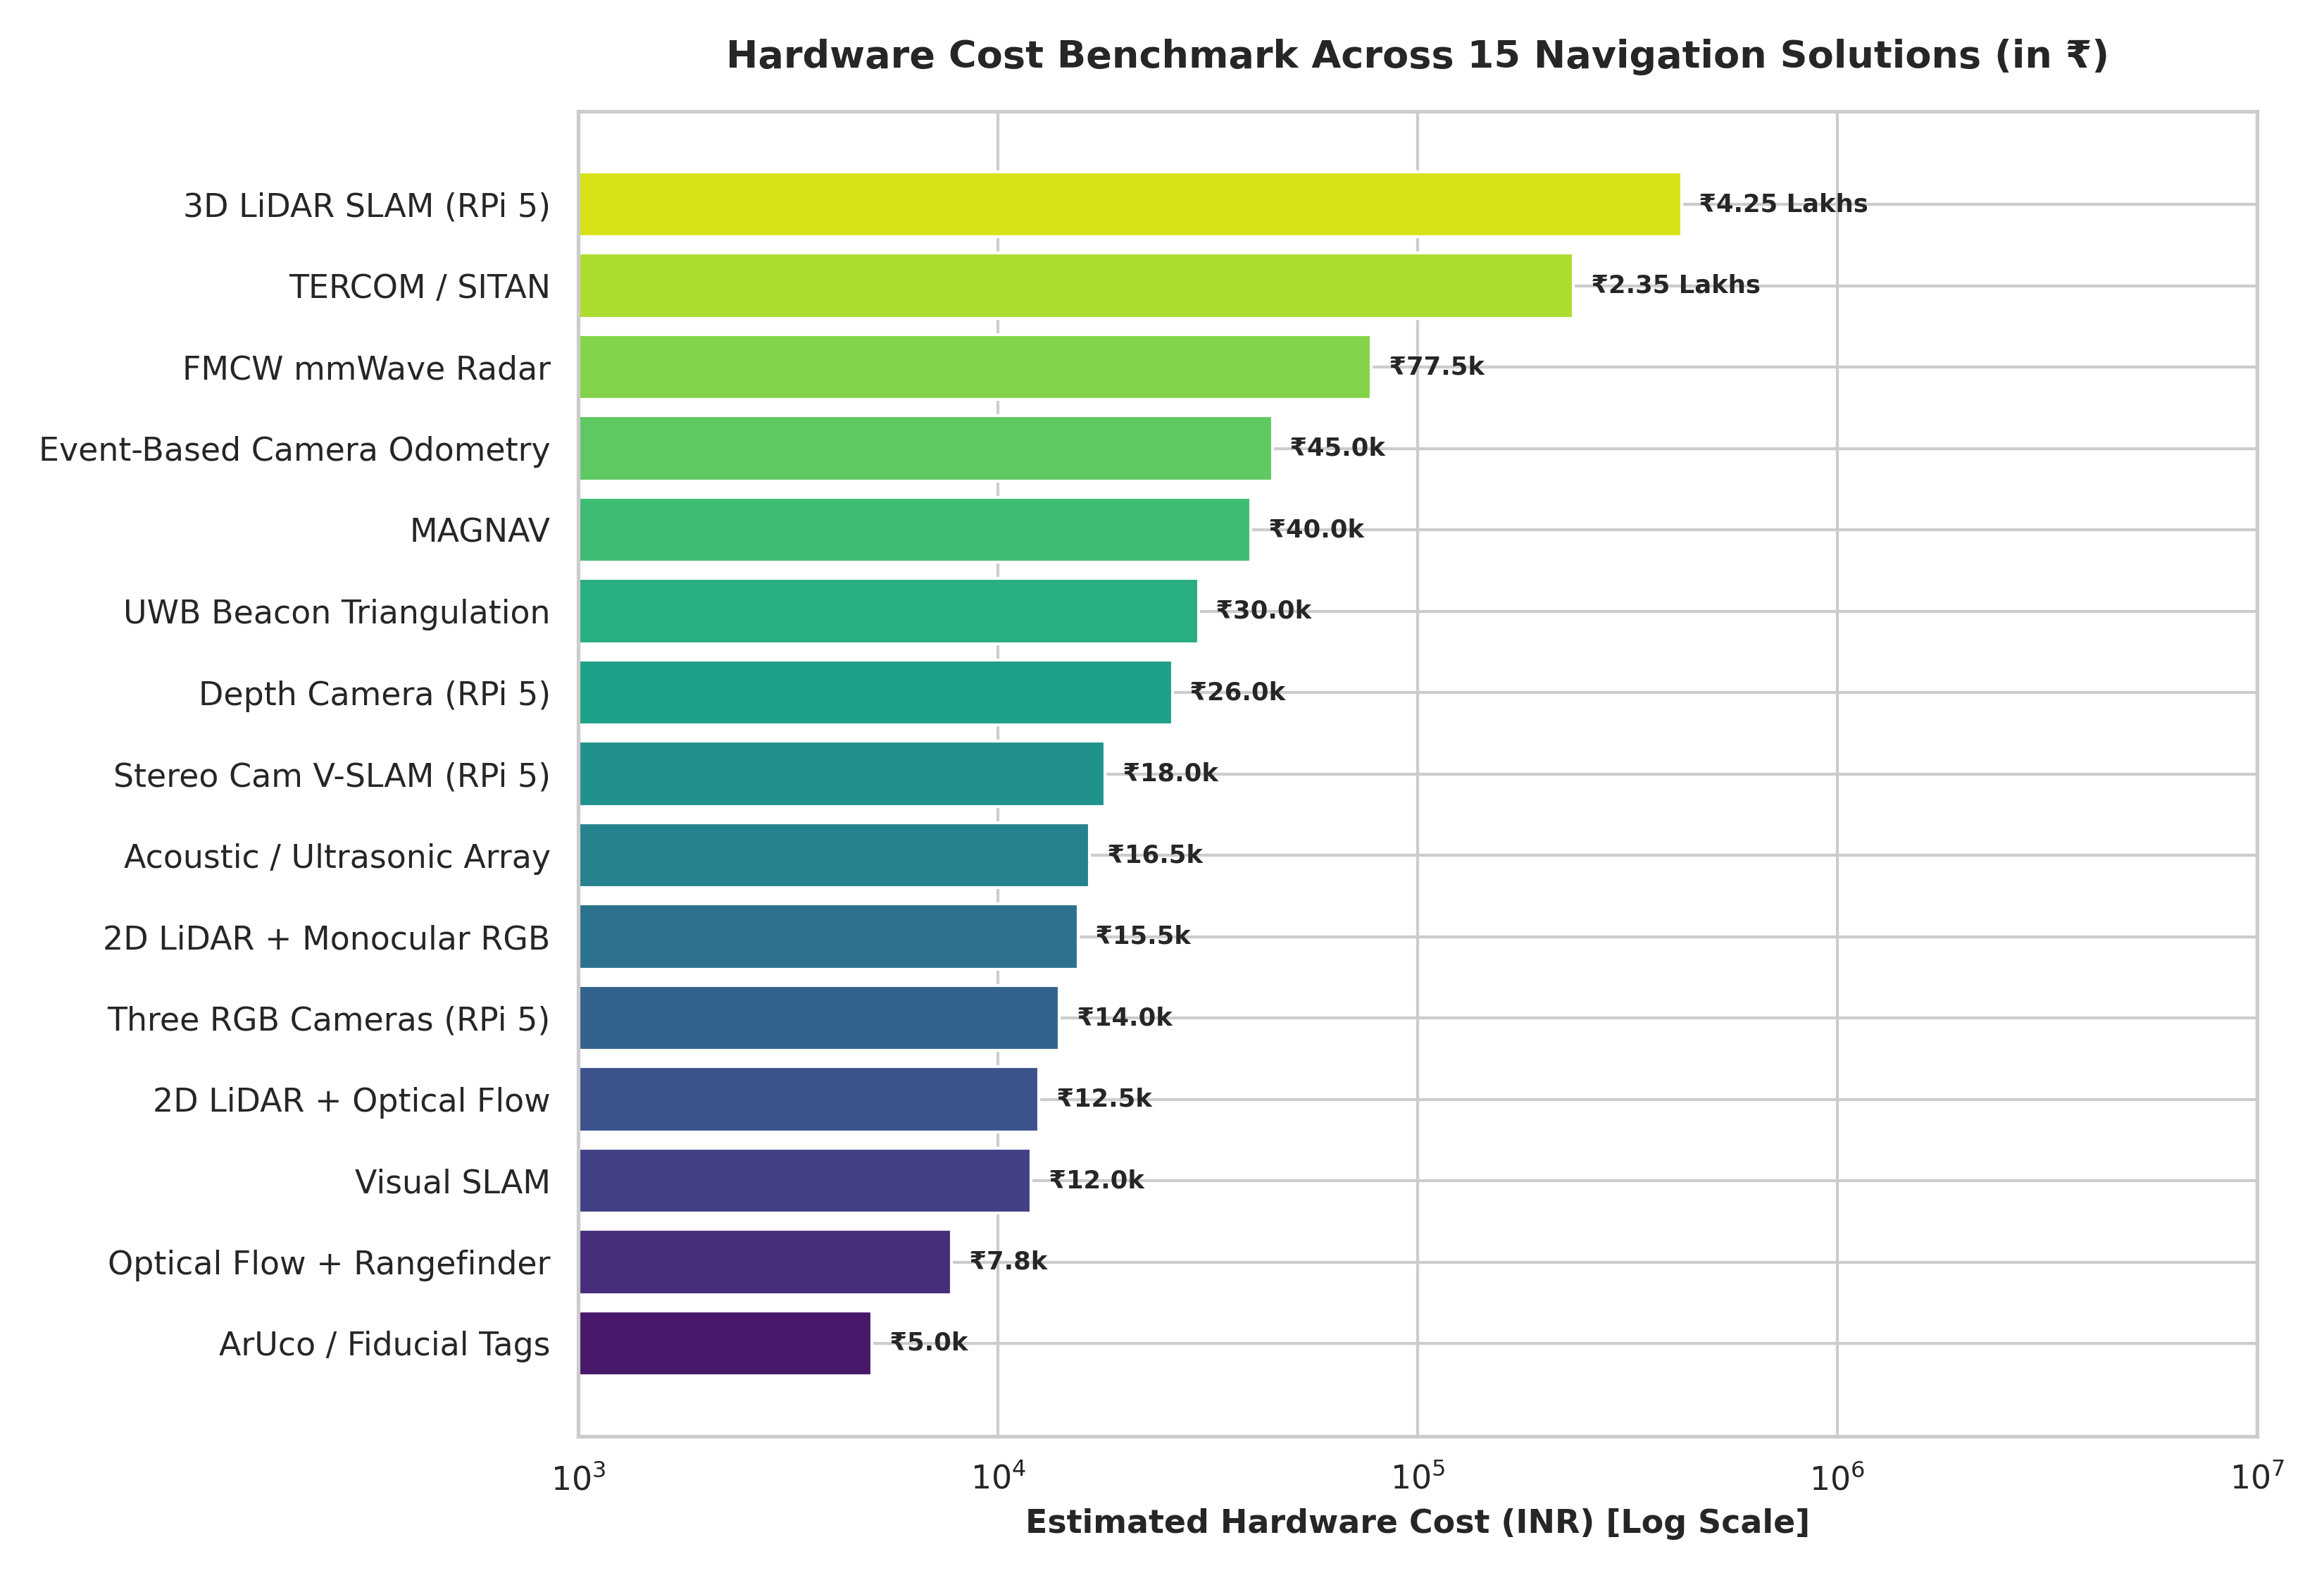
\includegraphics[width=\linewidth]{3_cost_benchmark_inr.png}
  \caption{Hardware cost per solution (INR, log scale).}
\end{subfigure}\hfill
\begin{subfigure}[t]{0.49\textwidth}
  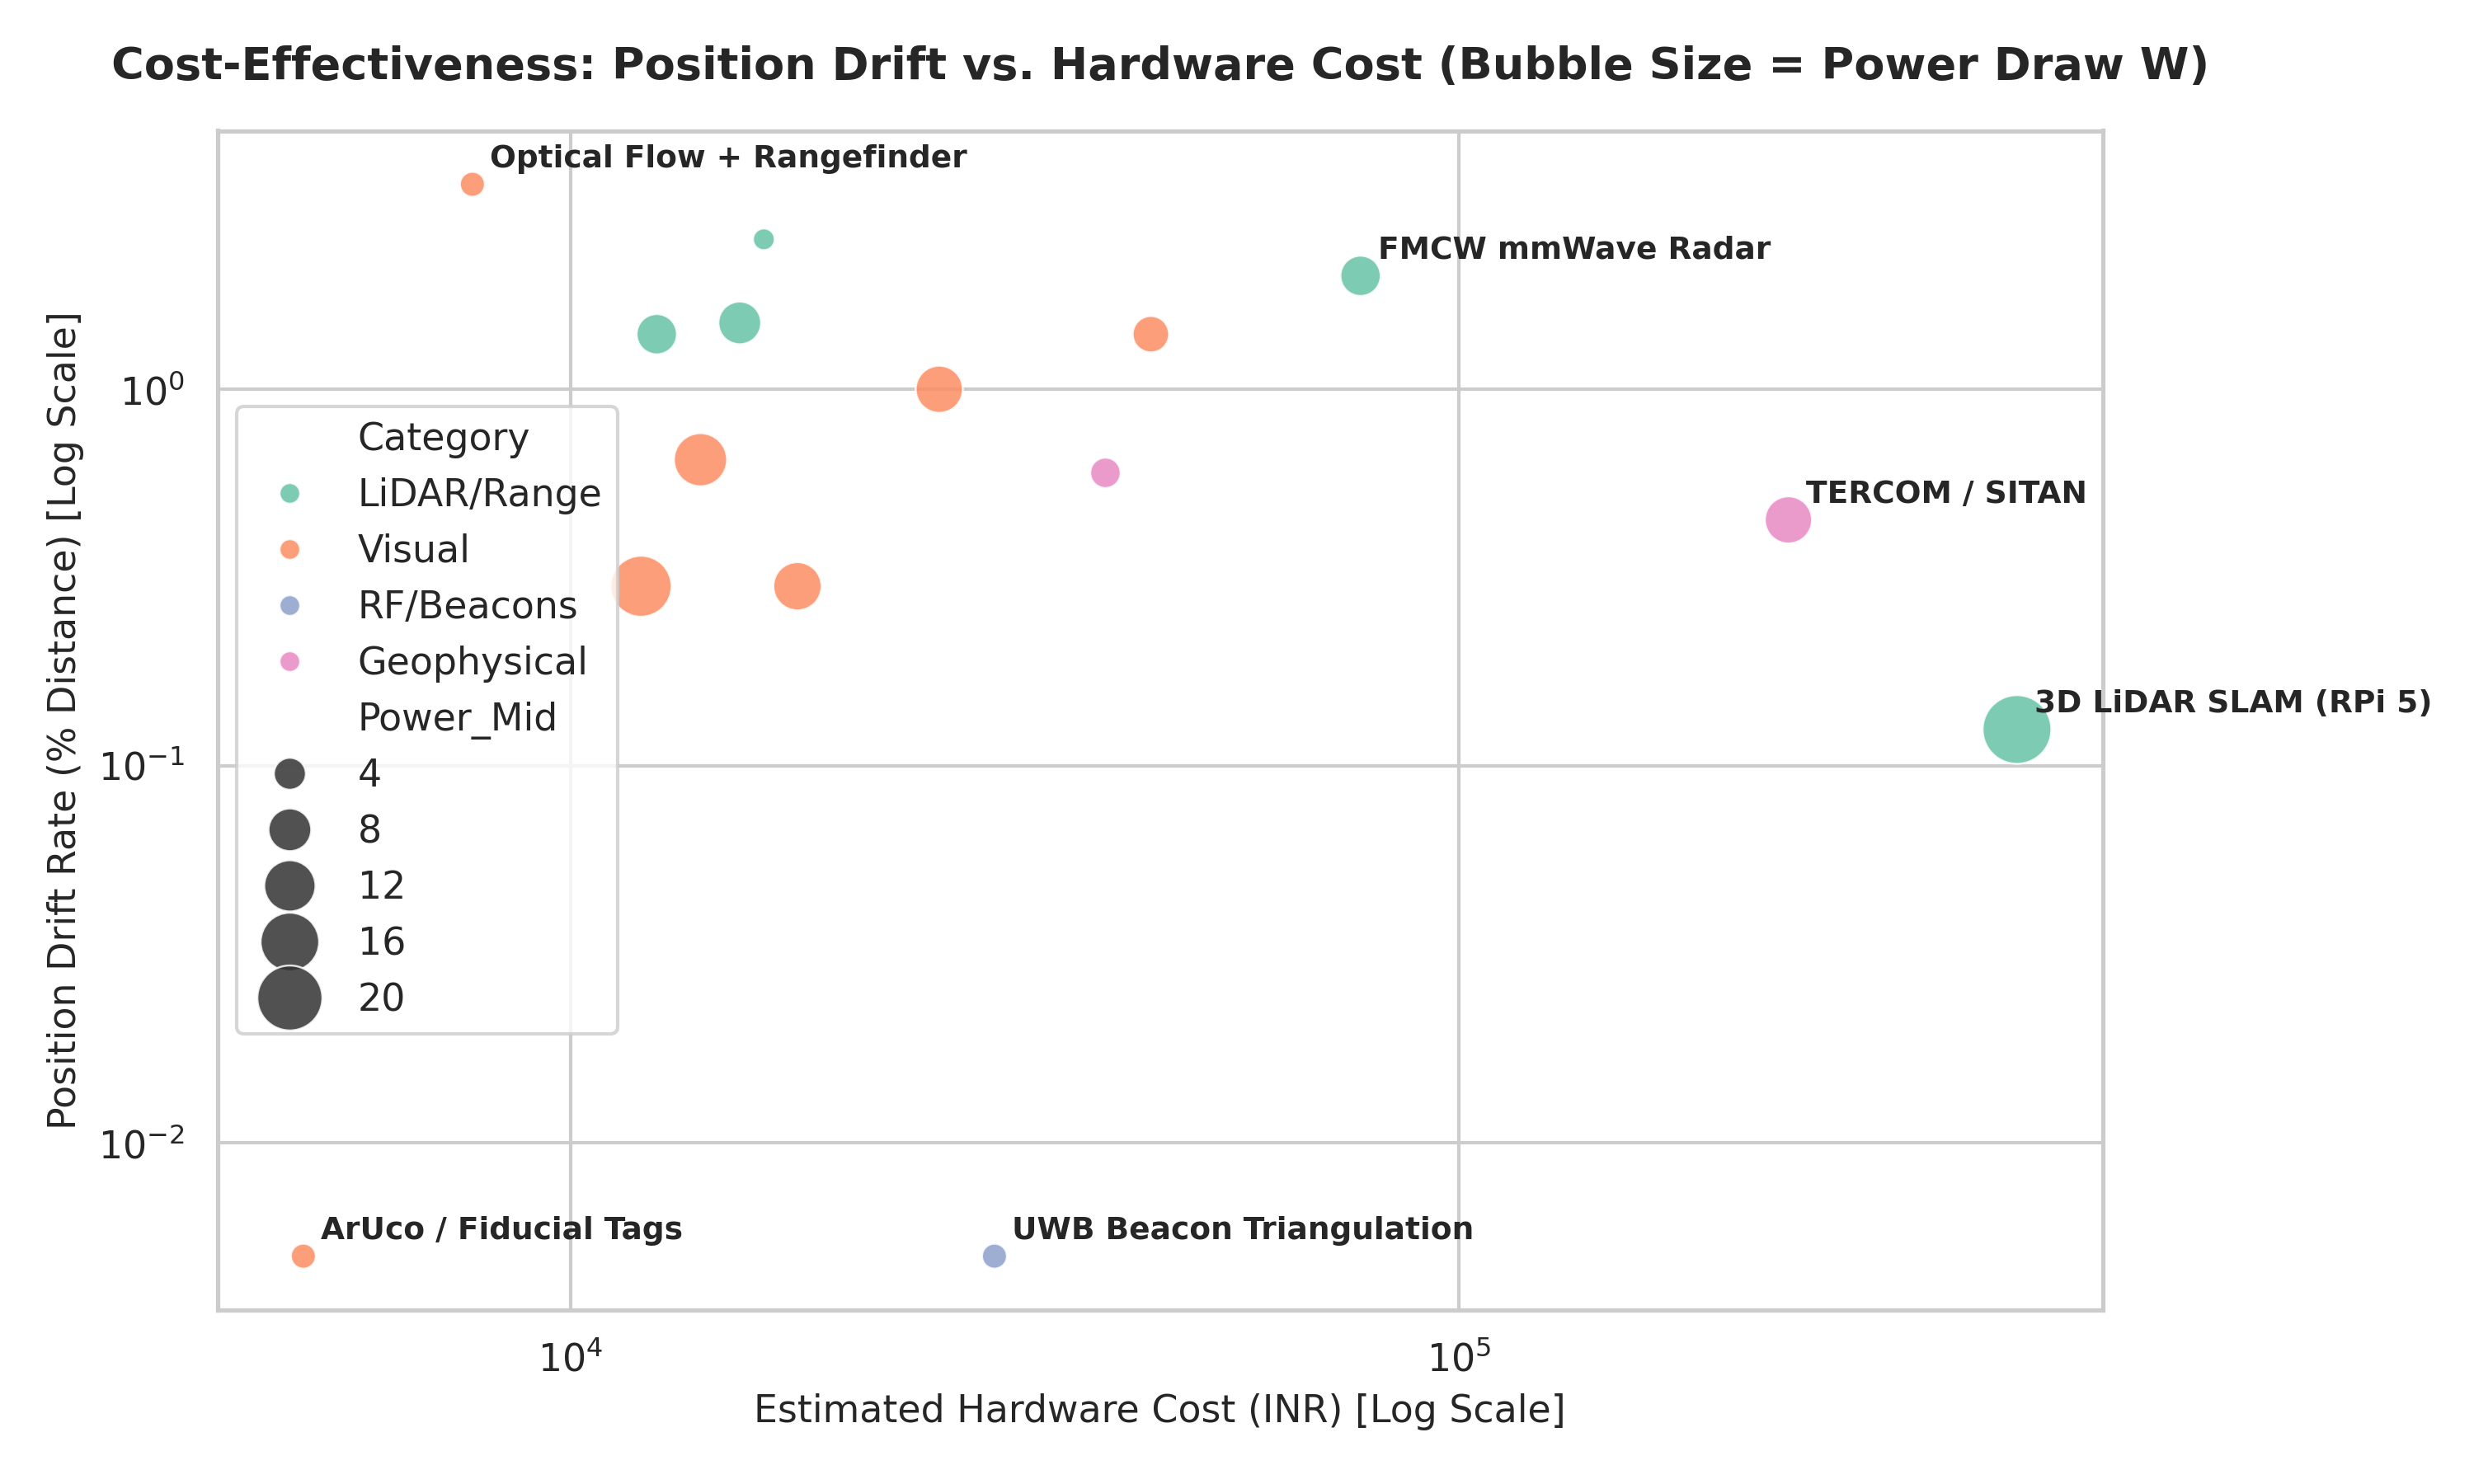
\includegraphics[width=\linewidth]{5_cost_effectiveness.png}
  \caption{Drift against cost (bubble size = power).}
\end{subfigure}

\vspace{2mm}
\begin{subfigure}[t]{0.49\textwidth}
  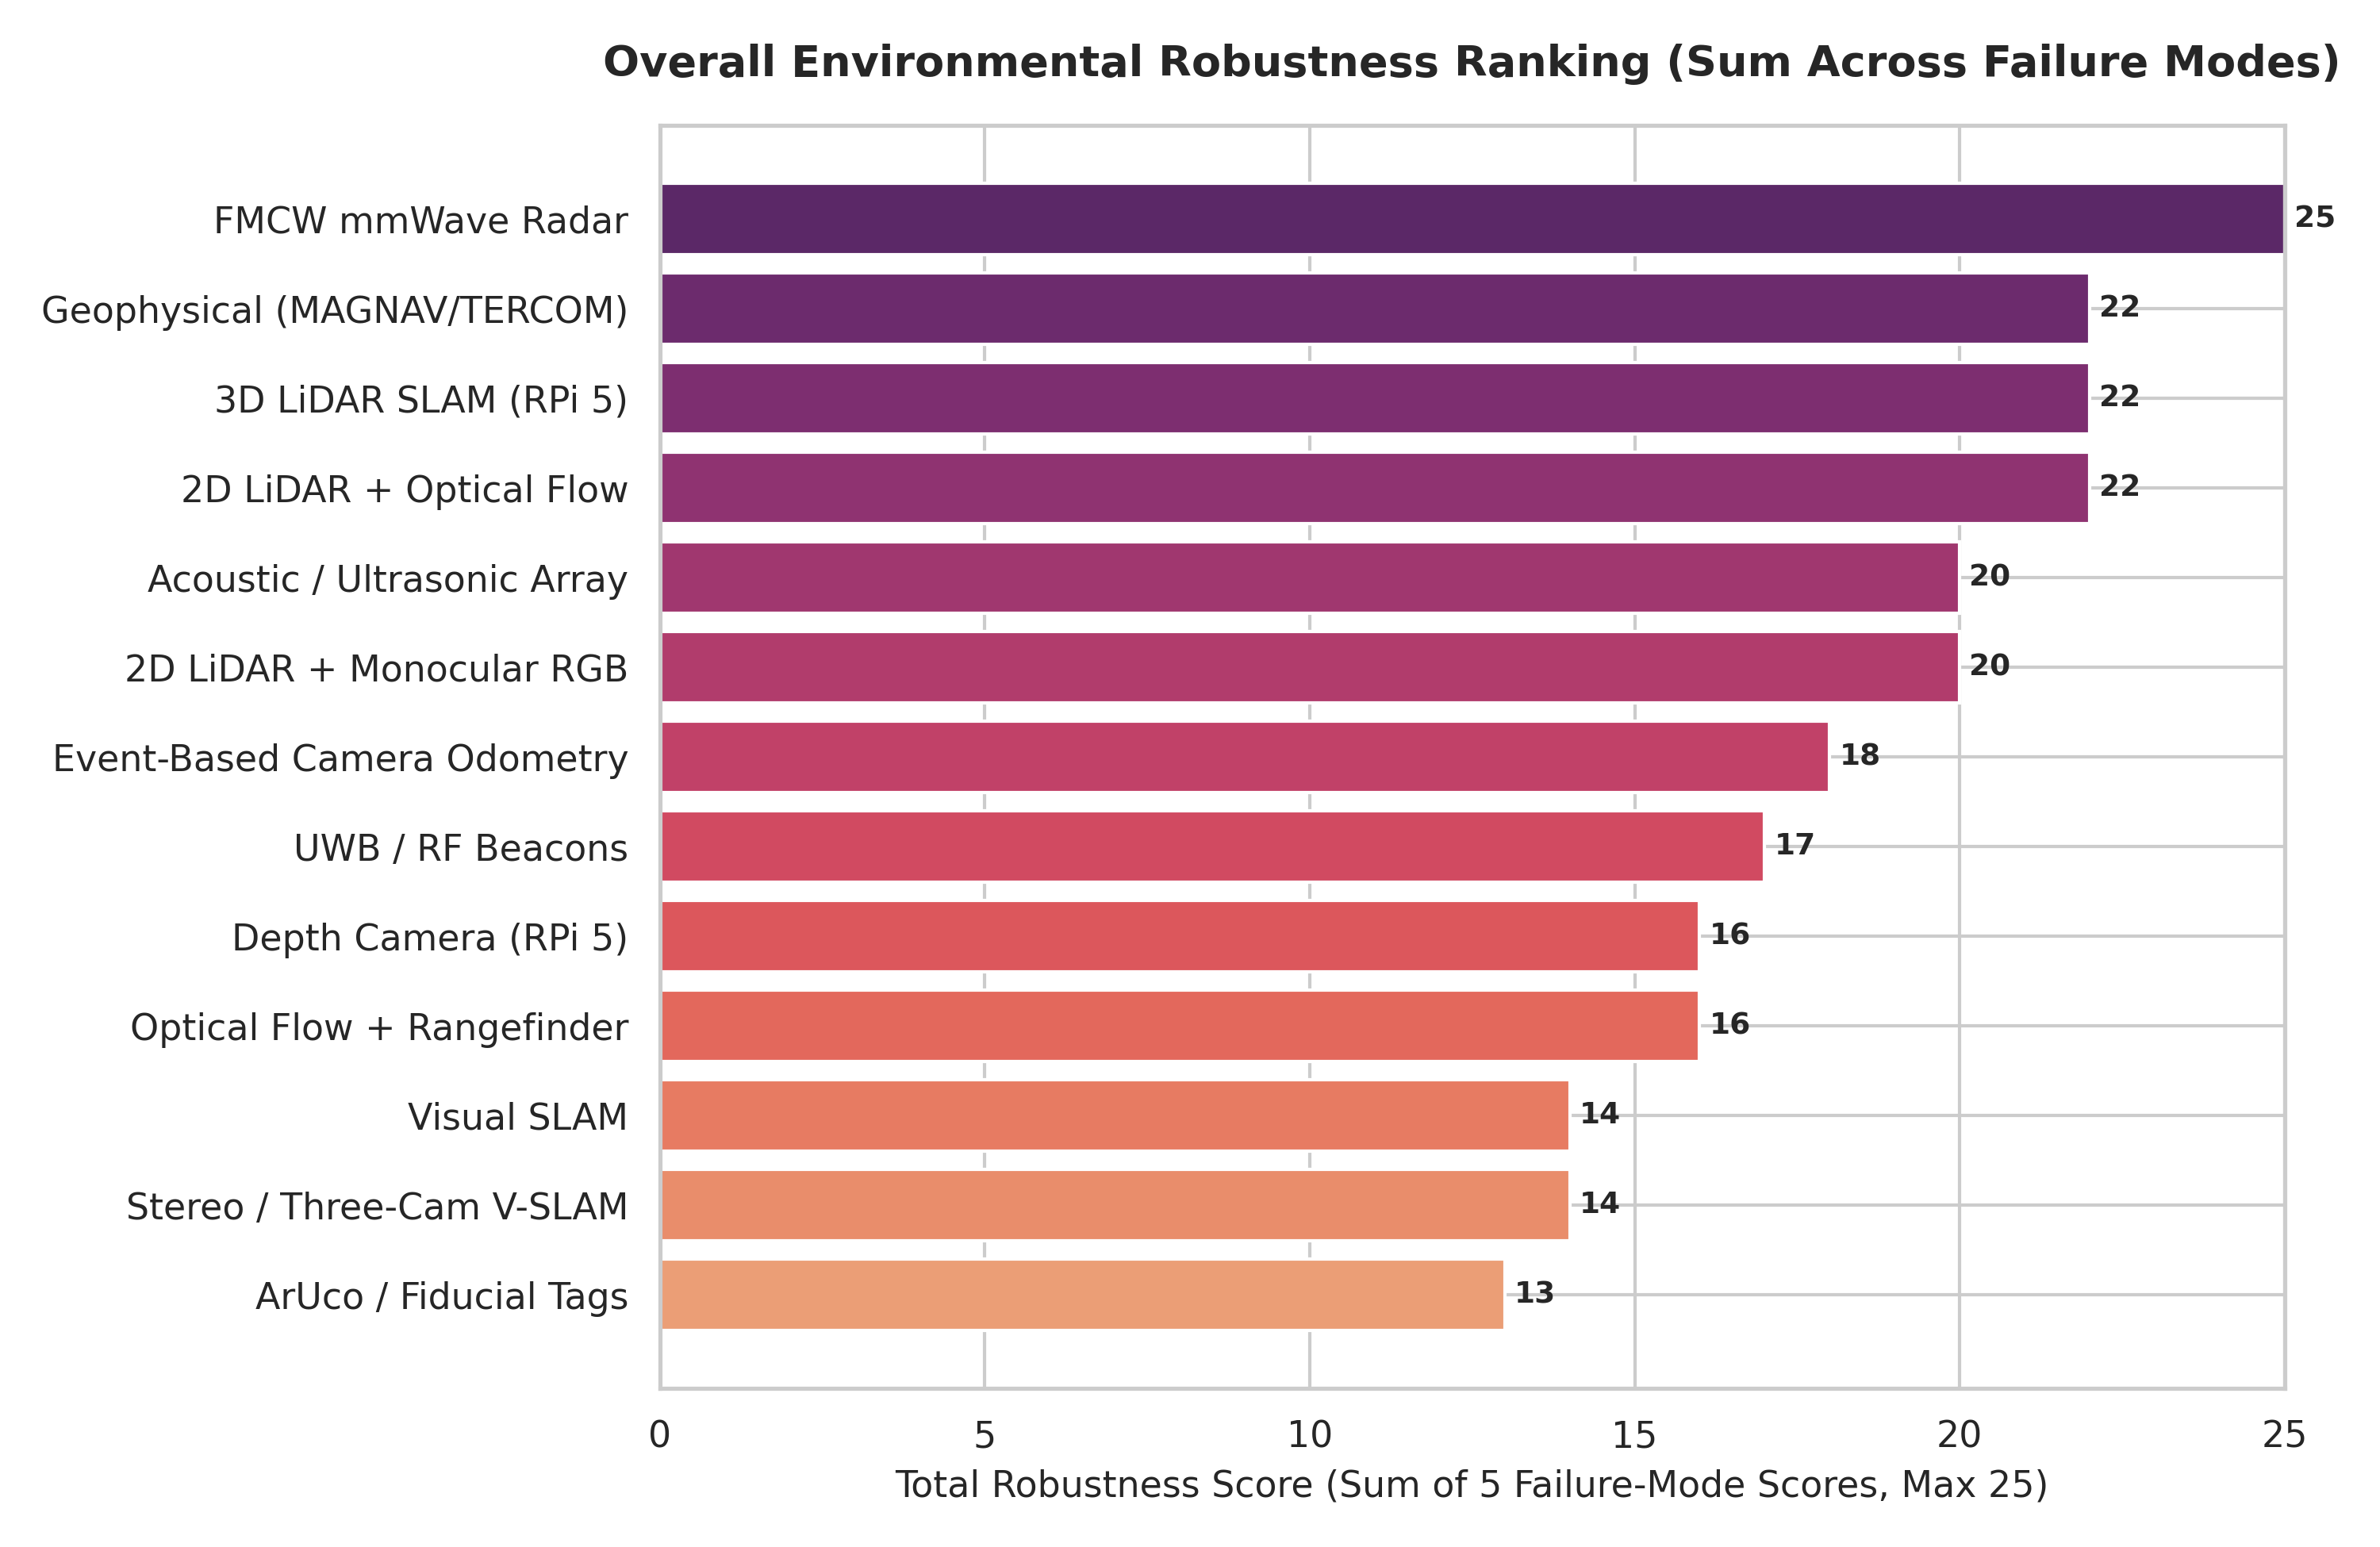
\includegraphics[width=\linewidth]{7_robustness_total.png}
  \caption{Total robustness score (sum of five failure modes).}
\end{subfigure}\hfill
\begin{subfigure}[t]{0.49\textwidth}
  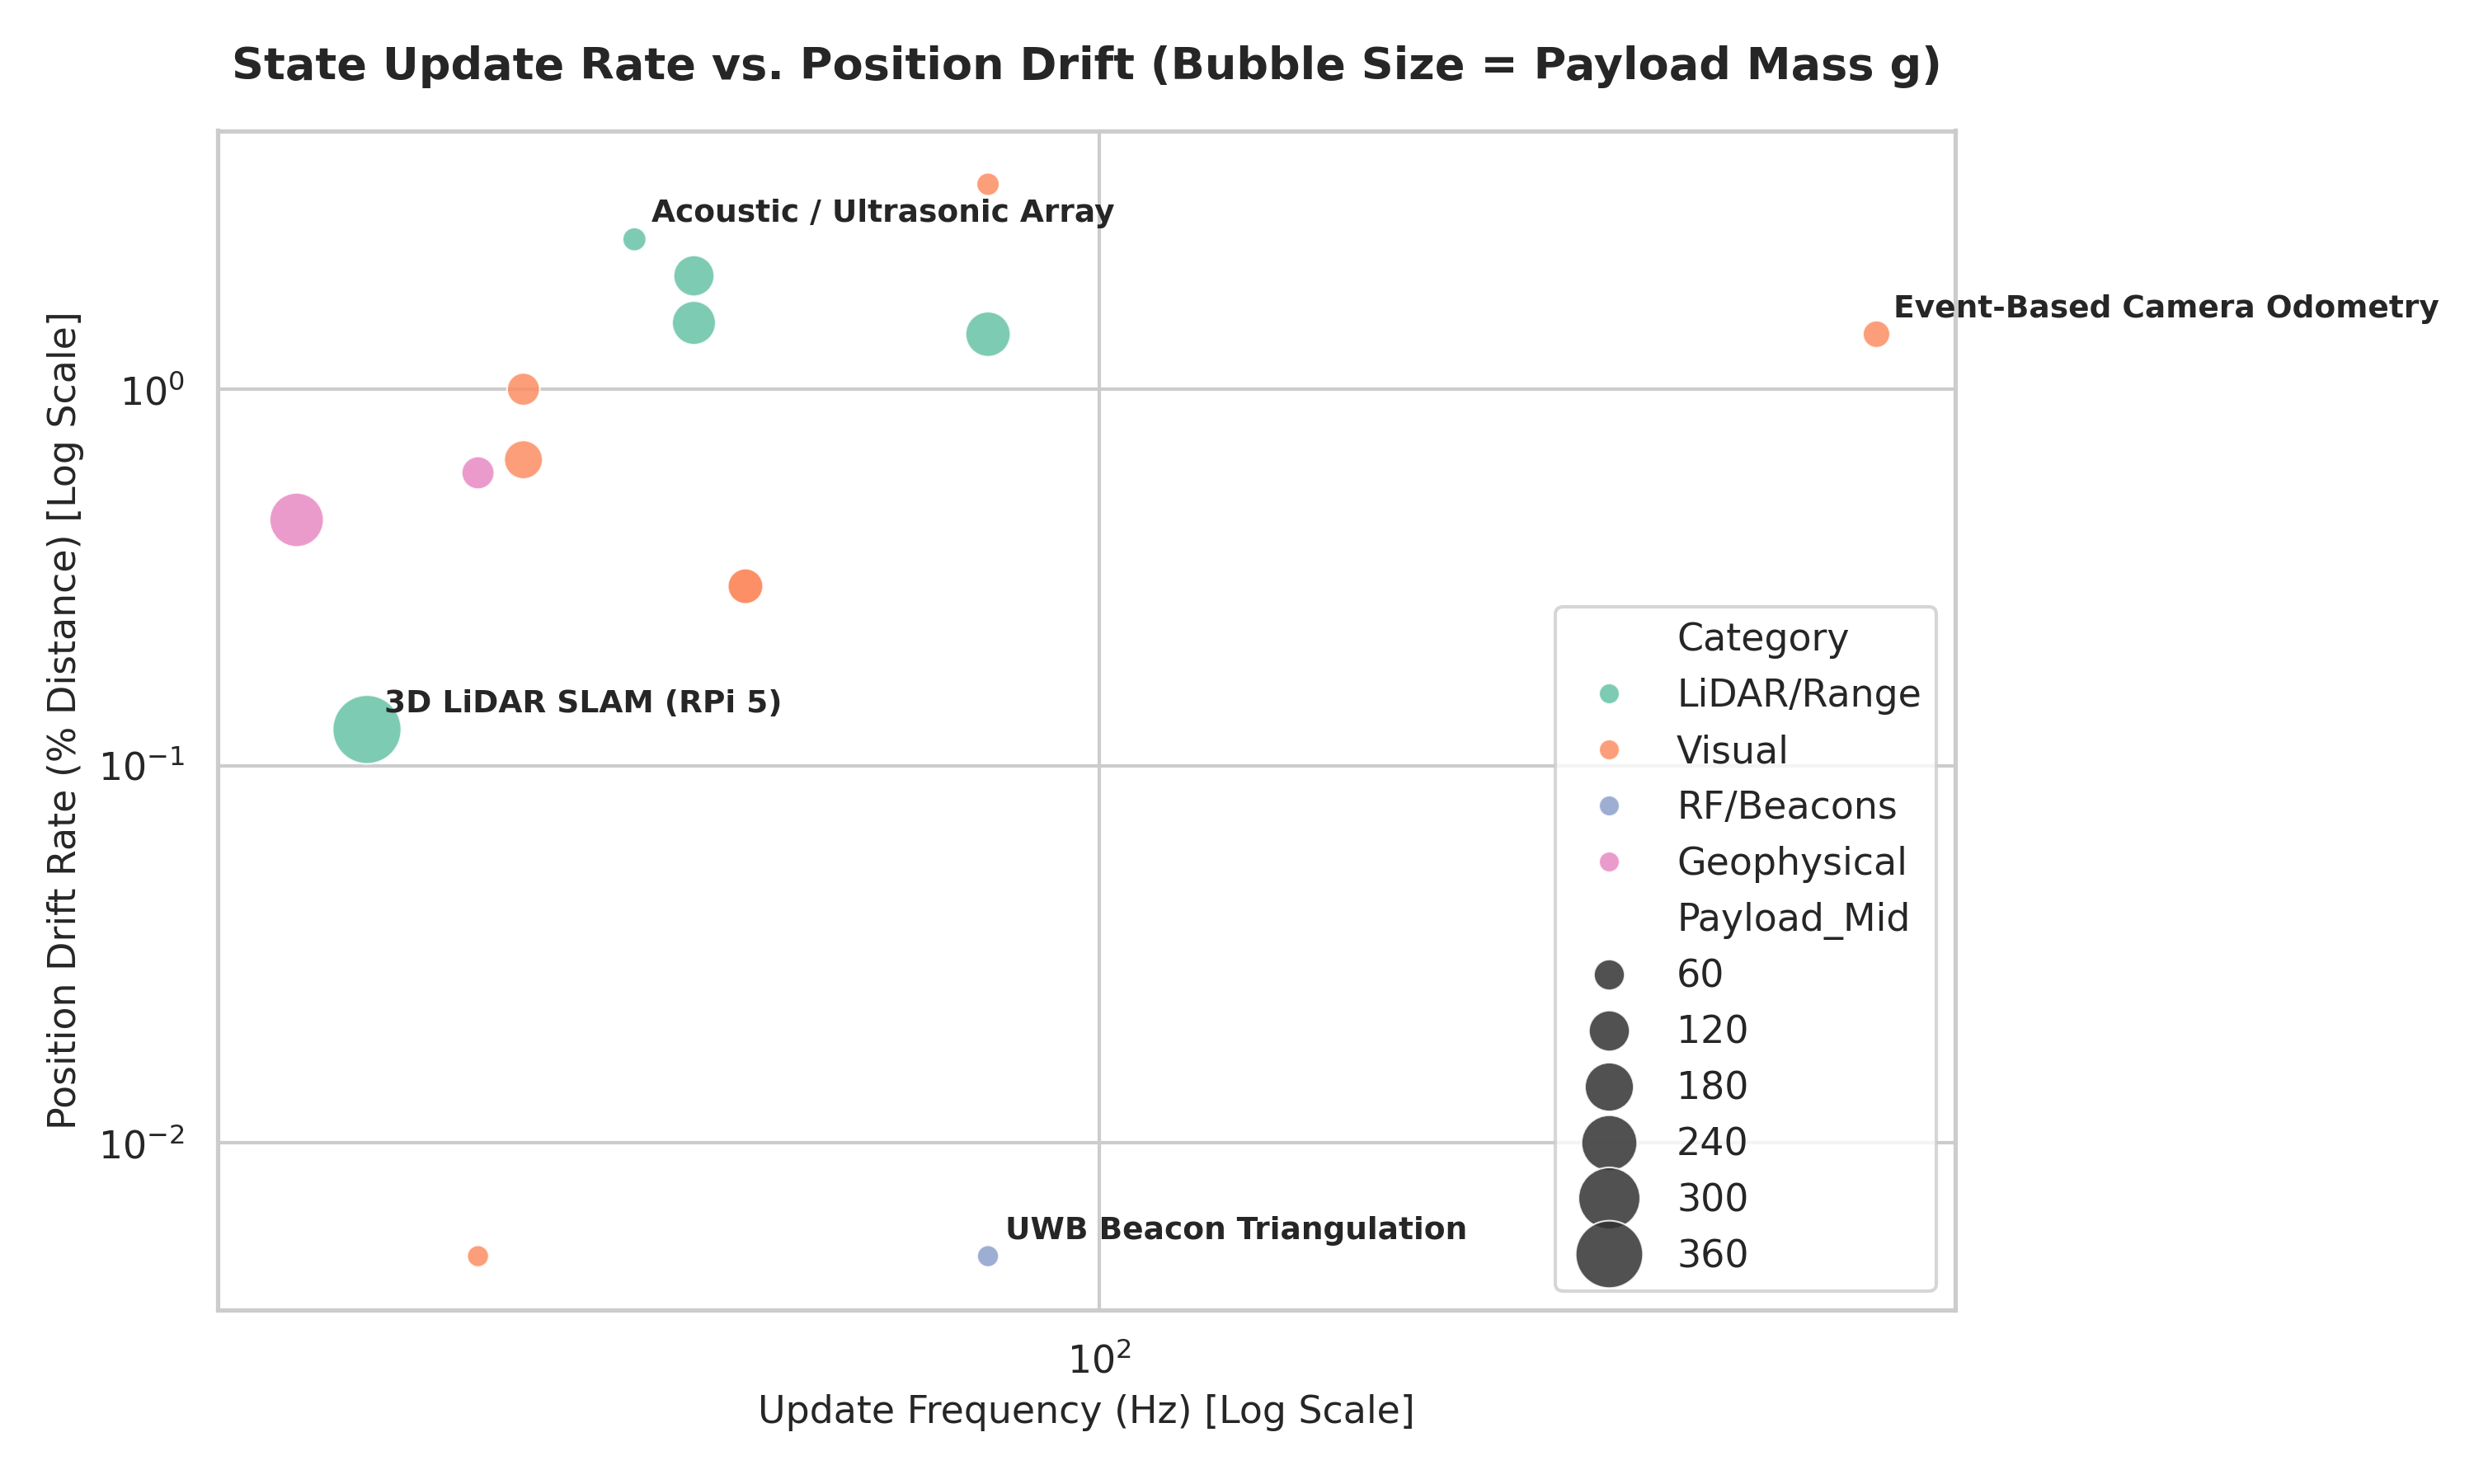
\includegraphics[width=\linewidth]{10_update_rate_vs_drift.png}
  \caption{Update rate against drift (bubble size = mass).}
\end{subfigure}
\caption{Further views of the same trade-study dataset (\cref{tab:solutions}), from
\code{scripts/analysis.py}. The values are screening estimates, not measurements.
Axes with drift or cost use log scales.}
\label{fig:trade2}
\end{figure}


\end{document}
